\newif\ifanon\anontrue    % set true to suppress names, etc.
\newif\iffull\fullfalse   % set true for long version

\documentclass[numbers]{sigplanconf}
\listfiles

% The following \documentclass options may be useful:

% preprint      Remove this option only once the paper is in final form.
% 10pt          To set in 10-point type instead of 9-point.
% 11pt          To set in 11-point type instead of 9-point.
% authoryear    To obtain author/year citation style instead of numeric.

\usepackage{amsmath}
\usepackage[table]{xcolor}
\usepackage{mathtools}
\usepackage{bussproofs}
\usepackage{amsthm}
\usepackage{csvsimple}
\usepackage{thmtools,thm-restate}
\usepackage{changepage}
\usepackage{booktabs}
\usepackage{amssymb}
\usepackage{enumitem}
\usepackage{multirow,bigdelim}
\usepackage{siunitx}
\usepackage{listings}
\usepackage{sansmath}
\usepackage{url}
\usepackage{flushend}
\usepackage{microtype}
\usepackage[utf8]{inputenc}
\usepackage{mathpartir}
\usepackage{empheq}
\usepackage{array}
\usepackage{pgfplots}
\usepackage{stmaryrd}
\usepackage{courier}
\usepackage{qtree}
\usepackage[normalem]{ulem}
\usepackage{relsize}

%%%% Hyperlinks – must come late!
\usepackage[pdftex,%
            pdfpagelabels,%
            linkcolor=blue,%
            citecolor=blue,%
            filecolor=blue,%
            urlcolor=blue]
           {hyperref}

% Colors
\definecolor{dkblue}{rgb}{0,0.1,0.5}
\definecolor{dkgreen}{rgb}{0,0.6,0}
\definecolor{dkred}{rgb}{0.6,0,0}
\definecolor{dkpurple}{rgb}{0.4,0,0.6}
\definecolor{olive}{rgb}{0.4, 0.4, 0.0}
\definecolor{teal}{rgb}{0.0,0.5,0.5}
\definecolor{orange}{rgb}{0.9,0.6,0.2}
\definecolor{lightyellow}{RGB}{255, 255, 179}
\definecolor{lightgreen}{RGB}{170, 255, 220}
\definecolor{teal}{RGB}{141,211,199}
\definecolor{darkbrown}{RGB}{121,37,0}

% remove whitespace before and after multicols
\setlength{\multicolsep}{0pt}

% renewtheorem https://tex.stackexchange.com/questions/103013/is-there-a-renewtheorem-equivalent-of-renewcommand-using-amsthm-and-not-ntheo
\makeatletter
\def\renewtheorem#1{%
  \expandafter\let\csname#1\endcsname\relax
  \expandafter\let\csname c@#1\endcsname\relax
  \gdef\renewtheorem@envname{#1}
  \renewtheorem@secpar
}
\def\renewtheorem@secpar{\@ifnextchar[{\renewtheorem@numberedlike}{\renewtheorem@nonumberedlike}}
\def\renewtheorem@numberedlike[#1]#2{\newtheorem{\renewtheorem@envname}[#1]{#2}}
\def\renewtheorem@nonumberedlike#1{  
\def\renewtheorem@caption{#1}
\edef\renewtheorem@nowithin{\noexpand\newtheorem{\renewtheorem@envname}{\renewtheorem@caption}}
\renewtheorem@thirdpar
}
\def\renewtheorem@thirdpar{\@ifnextchar[{\renewtheorem@within}{\renewtheorem@nowithin}}
\def\renewtheorem@within[#1]{\renewtheorem@nowithin[#1]}
\makeatother

\pgfplotsset{
% override style for non-boxed plots
    % which is the case for both sub-plots
    every non boxed x axis/.style={} 
}

\newenvironment{mathprooftree}
  {\varwidth{.9\textwidth}\centering\leavevmode}
  {\DisplayProof\endvarwidth}

\newcommand{\FINISH}[3]{\ifdraft\textcolor{#1}{[#2: #3]}\fi}
\newcommand{\bcp}[1]{\FINISH{dkred}{B}{#1}}
\newcommand{\BCP}[1]{\FINISH{dkred}{B}{\bf #1}}
\newcommand{\afm}[1]{\FINISH{dkgreen}{A}{#1}}
\newcommand{\dpw}[1]{\FINISH{dkblue}{D}{#1}}
\newcommand{\saz}[1]{\FINISH{orange}{S}{#1}}
\newcommand{\ksf}[1]{\FINISH{teal}{K}{#1}}
\newcommand{\revised}[1]{\FINISH{dkred}{#1}}

\newcommand{\IE}{\emph{i.e.}}
\newcommand{\EG}{\emph{e.g.}}
\newcommand{\ETC}{\emph{etc.}}

\theoremstyle{definition}
\renewtheorem{theorem}{Theorem}
\newtheorem{mylemma}{Lemma}
\renewtheorem{corollary}{Corollary}
\renewtheorem{conjecture}{Conjecture}
\renewtheorem{definition}{Definition}
\newtheorem{property}{Property}
\theoremstyle{plain}
\theoremstyle{remark}
\newtheorem{subcase}{Subcase}
\theoremstyle{remark}
\newtheorem{case}{Case}
\makeatletter
\@addtoreset{subcase}{case}
\@addtoreset{case}{mylemma}
\@addtoreset{case}{theorem}
\@addtoreset{case}{corollary}
\@addtoreset{case}{definition}
\@addtoreset{case}{definition}
\@removefromreset{theorem}{section}
\makeatother

\algnewcommand\algorithmicswitch{\textbf{switch}}
\algnewcommand\algorithmicmatch{\textbf{match}}
\algnewcommand\algorithmiccase{\textbf{case}}
\algnewcommand\algorithmicwith{\textbf{with}}
\algnewcommand\algorithmicforeach{\textbf{foreach}}
\algnewcommand\Assert[1]{\State \algorithmicassert(#1)}%
% New "environments"
\algdef{SE}[SWITCH]{Switch}{EndSwitch}[1]{\algorithmicmatch\ #1\ \algorithmicwith}{\algorithmicend\ \algorithmicswitch}%
\algdef{SE}[CASE]{Case}{EndCase}[1]{$|~$ #1 $\rightarrow$}{\algorithmicend\ \algorithmiccase}%
\algdef{SE}[FOREACH]{ForEach}{EndForEach}[2]{\algorithmicforeach\ #1 $\in$ #2}{\algorithmicend\ \algorithmicforeach}%
\algdef{SE}[CaseTwo]{CaseTwo}{EndCaseTwo}[2]{$|~$ #1 $\rightarrow$ #2}{\algorithmicend\ \algorithmiccase}%
\algtext*{EndSwitch}%
\algtext*{EndCase}%
\algtext*{EndCaseTwo}%
\algtext*{EndSecondCase}%
\algtext*{EndForEach}%



\newcommand{\CF}[1]{\ensuremath{\mathsf{#1}}}         % Code Font
\newcommand{\SmallCF}[1]{{\small \mathsf{#1}}}
\newcommand{\PCF}[1]{\textproc{#1}}
\newcommand{\VarCF}[1]{{\color{darkbrown} \CF{#1}}}
\newcommand{\StringCF}[1]{\CF{\textcolor{blue}{#1}}}
\newcommand{\KW}[1]{\CF{\textcolor{dkpurple}{#1}}}
\newcommand{\Regex}{\ensuremath{\mathit{S}}\xspace}         % Regular Expression
\newcommand{\RegexType}{\ensuremath{\textit{Regex}}}
\newcommand{\EquivRegexType}{\ensuremath{\textit{Regex}/\sim}}
\newcommand{\BooleanAnd}{\ensuremath{~\wedge~}}
\newcommand{\BooleanOr}{\ensuremath{\vee}}
\newcommand{\BooleanImplies}{\ensuremath{\Rightarrow}}
\newcommand{\Rewrite}{\ensuremath{\rightarrow}}
\newcommand{\RewriteAtom}{\ensuremath{\Rewrite_\Atom}}
\newcommand{\RewriteDNF}{\ensuremath{\Rewrite_\DNFRegex}}
\newcommand{\ConcatDNF}{\ensuremath{\odot}}
\newcommand{\ConcatDNFOf}[2]{\ensuremath{#1\ConcatDNF#2}}
\newcommand{\BigConcatDNF}{\ensuremath{\bigodot}}
\newcommand{\ConcatSequence}{\ensuremath{\odot_{\Sequence}}}
\newcommand{\ConcatSequenceOf}[2]{\ensuremath{#1\ConcatSequence#2}}
\newcommand{\ConcatPermutation}{\ensuremath{\odot}}
\newcommand{\ConcatPermutationOf}[2]{\ensuremath{#1\ConcatPermutation#2}}
\newcommand{\SwapPermutation}{\ensuremath{\circledS}}
\newcommand{\SwapPermutationOf}[2]{\ensuremath{#1\SwapPermutation#2}}
\newcommand{\DistributePermutation}{\ensuremath{\otimes}}
\newcommand{\DistributePermutationOf}[2]{\ensuremath{#1\DistributePermutation#2}}
\newcommand{\DistributeSwapPermutation}{\ensuremath{\otimes^{\mathit{s}}}}
\newcommand{\DistributeSwapPermutationOf}[2]{\ensuremath{#1\DistributeSwapPermutation#2}}
\newcommand{\ConcatSequenceLens}{\ensuremath{\odot_{\SequenceLens}}}
\newcommand{\ConcatSequenceLensOf}[2]{\ensuremath{#1\ConcatSequenceLens#2}}
\newcommand{\ConcatDNFLens}{\ensuremath{\odot}}
\newcommand{\ConcatDNFLensOf}[2]{\ensuremath{#1\ConcatDNFLens#2}}
\newcommand{\SwapSequenceLens}{\ensuremath{\circledS_{\SequenceLens}}}
\newcommand{\SwapSequenceLensOf}[2]{\ensuremath{#1\SwapSequenceLens#2}}
\newcommand{\SwapDNFLens}{\ensuremath{\circledS}}
\newcommand{\SwapDNFLensOf}[2]{\ensuremath{#1\SwapDNFLens#2}}
\newcommand{\RepeatDNFOfTimes}[1]{\ensuremath{^{#1}}}
\newcommand{\RepeatDNFOf}[2]{\ensuremath{{#2}\RepeatDNFOfTimes{#1}}}
\newcommand{\RepeatDNFLensOfTimes}[1]{\ensuremath{^{#1}}}
\newcommand{\RepeatDNFLensOf}[2]{\ensuremath{{#2}\RepeatDNFLensOfTimes{#1}}}
\newcommand{\OrDNF}{\ensuremath{\oplus}}
\newcommand{\OrDNFOf}[3]{\ensuremath{#1\OrDNF_{#3}#2}}
\newcommand{\OrDNFLens}{\ensuremath{\oplus}}
\newcommand{\OrDNFLensOf}[2]{\ensuremath{#1\OrDNFLens#2}}
\newcommand{\PutRSym}{\ensuremath{\mathit{putr}}}
\newcommand{\PutLSym}{\ensuremath{\mathit{putl}}}
\newcommand{\PutRSymOf}[1]{\ensuremath{\PutRSym \App #1}}
\newcommand{\PutLSymOf}[1]{\ensuremath{\PutLSym \App #1}}
\newcommand{\RegexAlt}{\ensuremath{\mathit{T}}\xspace}         % Regular Expression
\newcommand{\RegexAltAlt}{\ensuremath{\mathit{U}}\xspace}         % Regular Expression
\newcommand{\Or}{\ensuremath{~|~}}
\newcommand{\RegexOr}[2]{\ensuremath{#1\Or#2}}
\newcommand{\SubN}{\textsubscript{n}}
\newcommand{\RegexConcat}[2]{\ensuremath{#1\cdot#2}}
\newcommand{\EmptyString}{\ensuremath{\epsilon}}
\newcommand{\StringConcat}[2]{\ensuremath{#1\cdot#2}}
\newcommand{\HasSemantics}{\ensuremath{\triangleright}}
\newcommand{\DerivesLens}{\ensuremath{\vdash}}
\newcommand{\DerivesDNFLens}{\ensuremath{\vdash_{\DNFLens}}}
\newcommand{\DerivesSequenceLens}{\ensuremath{\vdash_{\SequenceLens}}}
\newcommand{\DerivesAtomLens}{\ensuremath{\vdash_{\AtomLens}}}
\newcommand{\DerivesStringRegex}{\ensuremath{\vdash}}
\newcommand{\DerivesAtomRewrite}{\ensuremath{\vdash}}
\newcommand{\DerivesDNFRewrite}{\ensuremath{\vdash}}
\newcommand{\Concat}{\ensuremath{\cdot}}
\newcommand{\Union}{\ensuremath{\cup}}
\newcommand{\Intersect}{\ensuremath{\cap}}
\newcommand{\BigUnion}{\ensuremath{\bigcup}}
\newcommand{\BigIntersect}{\ensuremath{\bigcap}}
\newcommand{\denot}[1]{\ensuremath{[ \! [#1] \! ]}}
\newcommand{\SemanticsOf}[1]{\ensuremath{[ \! [#1] \! ]}}
\newcommand{\SetOf}[1]{\ensuremath{\{#1\}}}
\newcommand{\RegexVariable}{\ensuremath{\mathit{U}}}   % User Defined
\newcommand{\RegexVariableAlt}{\ensuremath{\mathit{V}}}
\newcommand{\LensVariable}{\ensuremath{\mathit{L}}}
\newcommand{\ExampledRegex}{\ensuremath{\mathit{er}}} % Exampled Regex
\newcommand{\UnambigItOf}[1]{\ensuremath{#1^{*!}}}
\newcommand{\UnambigConcat}{\ensuremath{\Concat^!}}
\newcommand{\SequenceUnambigConcatOf}[1]{\ensuremath{\UnambigConcat(#1)}}
\newcommand{\UnambigConcatOf}[2]{\ensuremath{#1 \UnambigConcat #2}}
\newcommand{\UnambigOrOf}[2]{\ensuremath{\LanguageOf{#1} \cap \LanguageOf{#2} = \emptyset}}
\newcommand{\Atom}{\ensuremath{\mathit{A}}}          % Atoms
\newcommand{\AtomAlt}{\ensuremath{\mathit{B}}}
\newcommand{\AtomType}{\ensuremath{\mathit{Atom}}}
\newcommand{\App}{\ensuremath{\,}}
\newcommand{\Sequence}{\ensuremath{\mathit{SQ}}}
\newcommand{\SequenceType}{\ensuremath{\mathit{Sequence}}}
\newcommand{\LetIn}[2]{\ensuremath{\text{let } #1 = #2\text{ in }}}
\newcommand{\LetWhereIn}[3]{\ensuremath{\text{let } #1 = #2 \text{ where } #3 \text{ in }}}
\newcommand{\Where}{\ensuremath{\text{ where }}}
\newcommand{\ClauseAlt}{\ensuremath{\mathit{bl}}}       % Clauses
\newcommand{\SequenceAlt}{\ensuremath{\mathit{TQ}}}
\newcommand{\DNFRegex}{\ensuremath{\mathit{DS}}}         % Regular Expression
\newcommand{\DNFRegexAlt}{\ensuremath{\mathit{DT}}}    %Alt Regex
\newcommand{\DNFRegexType}{\ensuremath{\mathit{DNF}}}
\newcommand{\LensContext}{\ensuremath{\Gamma}}
\newcommand{\RegexContext}{\ensuremath{\Delta}}  % Context
\newcommand{\FullContext}{\ensuremath{\Delta, \Gamma}}
\newcommand{\String}{\ensuremath{\mathit{s}}\xspace}        % String
\newcommand{\StringAlt}{\ensuremath{\mathit{t}}}        % StringAlt
\newcommand{\StringAltAlt}{\ensuremath{\mathit{u}}}        % StringAltAlt
\newcommand{\ExampleNumberList}{\ensuremath{\mathit{enl}}} %Example Number List
\newcommand{\ExampleNumberListList}{\ensuremath{\mathit{enll}}}
\newcommand{\ExampleStringList}{\ensuremath{\mathit{esl}}}
\newcommand{\StringList}{\ensuremath{\mathit{sl}}}
\newcommand{\Natural}{\ensuremath{\mathit{n}}}
\newcommand{\Interleaving}[1]{\ensuremath{\mathit{interleaving}(#1)}}
\newcommand{\Interleave}{\ensuremath{\mathit{interleave}}}
\newcommand{\BinaryInterleave}[2]{\ensuremath{\mathit{interleave}(#1,#2)}}
\newcommand{\NAryInterleave}[2]{\ensuremath{\mathit{interleave}(#1,\ldots,#2)}}
\newcommand{\Combine}{\ensuremath{\mathit{combine}}}
\newcommand{\List}{\ensuremath{\mathit{l}}}
\newcommand{\ValidCombine}[2]{\ensuremath{\mathit{validcombine}(#1,#2)}}
\newcommand{\ValidRegexContext}[2]{\ensuremath{\mathit{validregexcontext}(#1,#2)}}
\newcommand{\Parent}[1]{\ensuremath{\mathit{parent}(#1)}}
\newcommand{\Parented}[1]{\ensuremath{mathit{parented}(#1)}}
\newcommand{\CombineString}[1]{\ensuremath{\mathit{combine}_{\ExampleStringList}(#1)}}
\newcommand{\CombineList}[1]{\ensuremath{\mathit{combine}_{\ExampleNumberListList}(#1)}}
\newcommand{\Length}[1]{\ensuremath{\mathit{len}(#1)}}
\newcommand{\Language}{\ensuremath{L}}
\newcommand{\LanguageOf}[1]{\ensuremath{\mathcal{L}(#1)}}
\newcommand{\LanguageUnderContextOf}[2]{\ensuremath{\Language{}_{#1}(#2)}}
\newcommand{\ParseTree}{\ensuremath{\mathit{p}}}
\newcommand{\ParseTreeAlt}{\ensuremath{\mathit{q}}}
\newcommand{\ParseTrees}{\ensuremath{\mathit{ps}}}
\newcommand{\ParseTreeAlts}{\ensuremath{\mathit{qs}}}
\newcommand{\StarParse}[1]{\ensuremath{\mathit{starparse}(#1)}}
\newcommand{\LeftChoiceParse}[1]{\ensuremath{\mathit{l}.(#1)}}
\newcommand{\RightChoiceParse}[1]{\ensuremath{\mathit{r}.(#1)}}
\newcommand{\RangeExcInc}[2]{\ensuremath{(#1,#2]}}
\newcommand{\RangeIncInc}[2]{\ensuremath{[#1,#2]}}

\newcommand{\Lens}{\ensuremath{\mathit{\ell}}\xspace}
\newcommand{\AtomLens}{\ensuremath{\mathit{al}}}
\newcommand{\IterateAtomType}{\textit{Iterate}}
\newcommand{\ConcatedAtomsLens}{\ensuremath{\mathit{cal}}}
\newcommand{\OredClausesLens}{\ensuremath{\mathit{ocl}}}
\newcommand{\ClauseLens}{\ensuremath{\mathit{cll}}}
\newcommand{\SequenceLens}{\ensuremath{\mathit{sql}}}
\newcommand{\SequenceLensType}{\ensuremath{\mathit{SequenceLens}}}
\newcommand{\DNFLens}{\ensuremath{\mathit{dl}}}
\newcommand{\DNFLensType}{\ensuremath{\mathit{DNFLens}}}
\newcommand{\AtomLensType}{\ensuremath{\mathit{AtomLens}}}
\newcommand{\SynSim}[2]{\ensuremath{#1 \sim_{\mathit{sym}} #2}}
\newcommand{\ExdSynSim}[3]{\ensuremath{#2 \sim_{\mathit{sym},#1} #3}}

\newcommand{\PermutationSetOf}[1]{\ensuremath{S_{#1}}}
\newcommand{\Permutation}{\ensuremath{\sigma}}

\newcommand{\Star}{\ensuremath{^*}}
\newcommand{\StarOf}[1]{\ensuremath{{#1}\Star}}
\newcommand{\ConstLens}{\ensuremath{\mathit{const}}}
\newcommand{\ConstLensOf}[2]{\ensuremath{\ConstLens(#1,#2)}}
\newcommand{\ConcatLens}{\ensuremath{\KW{concat}}}
\newcommand{\ConcatLensOf}[2]{\ensuremath{\ConcatLens(#1,#2)}}
\newcommand{\ConcatLensShortOf}[2]{\ensuremath{\mathit{c}(#1,#2)}}
\newcommand{\SwapLens}{\ensuremath{\KW{swap}}\xspace}
\newcommand{\SwapLensOf}[2]{\ensuremath{\SwapLens(#1,#2)}}
\newcommand{\SwapLensShortOf}[2]{\ensuremath{\mathit{s}(#1,#2)}}
\newcommand{\OrLens}{\ensuremath{\KW{or}}\xspace}
\newcommand{\OrLensOf}[2]{\ensuremath{\OrLens(#1,#2)}}
\newcommand{\IdentityLens}{\ensuremath{\KW{id}}}
\newcommand{\IdentityLensOf}[1]{\ensuremath{\IdentityLens(#1)}}
\newcommand{\IdentityLensShortT}{\ensuremath{\mathit{id}}}
\newcommand{\IdentityLensShortOf}[1]{\ensuremath{\IdentityLensShortT_{#1}}}
\newcommand{\IterateLens}{\ensuremath{\KW{iterate}}\xspace}
\newcommand{\IterateLensOf}[1]{\ensuremath{\mathit{\IterateLens(#1)}}}
\newcommand{\Identity}{\ensuremath{\mathit{id}}}
\newcommand{\Compose}{\ensuremath{\circ}}
\newcommand{\ComposeLensOf}[2]{\ensuremath{#1\mathrel{;}#2}}
\newcommand{\Disconnect}{\ensuremath{\KW{disc}}\xspace}
\newcommand{\DisconnectOf}[4]{\ensuremath{\Disconnect(#1,#2,#3,#4)}}
\newcommand{\MergeL}{\ensuremath{\KW{merge\_left}}\xspace}
\newcommand{\MergeLOf}[2]{\ensuremath{\MergeL(#1,#2)}}
\newcommand{\MergeR}{\ensuremath{\KW{merge\_right}}\xspace}
\newcommand{\MergeROf}[2]{\ensuremath{\MergeR(#1,#2)}}
\newcommand{\Invert}{\ensuremath{\KW{invert}}}
\newcommand{\InvertOf}[1]{\ensuremath{\Invert(#1)}}

% GRAMMAR OPERATORS
\newcommand{\GBar}{\ensuremath{~|~}}
\newcommand{\GIndent}{\hspace{.5in}}
\newcommand{\GEq}{\ensuremath{::=~}}
\newcommand{\GEmp}{\ensuremath{\cdot}}
\newcommand{\Perm}{\ensuremath{\mathit{Perm}}}
\newcommand{\Nats}{\ensuremath{\mathbb{N}}}

\newcommand{\InverseOf}[1]{\ensuremath{#1^{-1}}}
\newcommand{\FloorOf}[1]{\ensuremath{\lfloor#1\rfloor}}
\newcommand{\CeilOf}[1]{\ensuremath{\lceil#1\rceil}}
\newcommand{\OfType}{\ensuremath{:}}
\newcommand{\OfRewritelessType}{\ensuremath{\,\,\tilde{\OfType}\,\,}}
\newcommand{\MapsBetweenTypeOf}[2]{\ensuremath{#1 \Leftrightarrow #2}}
\newcommand{\ArrowTypeOf}[2]{\ensuremath{#1 \rightarrow #2}}
\newcommand{\SizeOf}[1]{\ensuremath{|#1|}}

\newcommand{\ToDNFRegex}{\ensuremath{\Downarrow}}
\newcommand{\ToDNFRegexOf}[1]{\ensuremath{\ToDNFRegex\mkern-4mu #1}}
\newcommand{\ToRegex}{\ensuremath{\Uparrow}}
\newcommand{\ToRegexOf}[1]{\ensuremath{\ToRegex\mkern-4mu #1}}

\newcommand{\SuchThat}{\ensuremath{~|~}}
\newcommand{\That}{\ensuremath{~.~}}
\newcommand{\Given}{\ensuremath{~|~}}

\newcommand{\LeftQuotientOf}[2]{\ensuremath{#1\backslash#2}}
\newcommand{\RightQuotientOf}[2]{\ensuremath{#1\slash#2}}

\newcommand{\SuffixOf}[1]{\ensuremath{S_{#1}}}
\newcommand{\PrefixOf}[1]{\ensuremath{P_{#1}}}

\newcommand{\ComplementOf}[1]{\ensuremath{\bar{#1}}}

\newcommand{\Alphabet}{\ensuremath{\Sigma}}
\newcommand{\Character}{\ensuremath{c}}
\newcommand{\CharacterAlt}{\ensuremath{d}}

\newcommand{\SequenceLeft}{\ensuremath{[}}
\newcommand{\SequenceRight}{\ensuremath{]}}
\newcommand{\SequenceOf}[1]{\ensuremath{\SequenceLeft#1\SequenceRight}}
\newcommand{\SeqSep}{\ensuremath{\mkern-1mu\Concat\mkern-1mu}}
\newcommand{\DNFLeft}{\ensuremath{\langle}}
\newcommand{\DNFRight}{\ensuremath{\rangle}}
\newcommand{\DNFOf}[1]{\ensuremath{\DNFLeft#1\DNFRight}}
\newcommand{\DNFSep}{\ensuremath{\Or}}
\newcommand{\SequenceLensLeft}{\ensuremath{[}}
\newcommand{\SequenceLensRight}{\ensuremath{]}}
\newcommand{\SequenceLensOf}[1]{\ensuremath{\SequenceLensLeft#1\SequenceLensRight}}
\newcommand{\SeqLSep}{\ensuremath{\mkern-1mu\Concat\mkern-1mu}}
\newcommand{\DNFLensLeft}{\ensuremath{\langle}}
\newcommand{\DNFLensRight}{\ensuremath{\rangle}}
\newcommand{\DNFLensOf}[1]{\ensuremath{\DNFLensLeft#1\DNFLensRight}}
\newcommand{\DNFLSep}{\ensuremath{\Or}}


\newcommand{\ConstantLensRule}{\textsc{Constant Lens}}
\newcommand{\IdentityLensRule}{\textsc{Identity Lens}}
\newcommand{\IterateLensRule}{\textsc{Iterate Lens}}
\newcommand{\ConcatLensRule}{\textsc{Concat Lens}}
\newcommand{\SwapLensRule}{\textsc{Swap Lens}}
\newcommand{\OrLensRule}{\textsc{Or Lens}}
\newcommand{\ComposeLensRule}{\textsc{Compose Lens}}
\newcommand{\RewriteRegexLensRule}{\textsc{Rewrite Regex Lens}}

\newcommand{\AtomUnrollstarLeftRule}{\textsc{Atom Unrollstar\SubLeft}}
\newcommand{\AtomUnrollstarRightRule}{\textsc{Atom Unrollstar\SubRight}}
\newcommand{\ParallelAtomStructuralRewriteRule}{\textsc{Parallel Atom Structural Rewrite}}
\newcommand{\ParallelSwapAtomStructuralRewriteRule}{\textsc{Parallel Swap Atom Structural Rewrite}}
\newcommand{\AtomStructuralRewriteRule}{\textsc{Atom Structural Rewrite}}
\newcommand{\DNFStructuralRewriteRule}{\textsc{DNF Structural Rewrite}}
\newcommand{\ParallelDNFStructuralRewriteRule}{\textsc{Parallel DNF Structural Rewrite}}
\newcommand{\ParallelSwapDNFStructuralRewriteRule}{\textsc{Parallel Swap DNF Structural Rewrite}}
\newcommand{\IdentityRewriteRule}{\textsc{Identity Rewrite}}
\newcommand{\DNFReorderRule}{\textsc{DNF Reorder}}

\newcommand{\SequenceLensRule}{\textsc{Sequence Lens}}
\newcommand{\AtomLensRule}{\textsc{Atom Lens}}
\newcommand{\DNFLensRule}{\textsc{DNF Lens}}
\newcommand{\RewriteDNFRegexLensRule}{\textsc{Rewrite DNF Regex Lens}}

\newcommand{\SubLeft}{\textsubscript{L}}
\newcommand{\SubRight}{\textsubscript{R}}

\newcommand{\Set}{\ensuremath{\mathit{S}}}

\newcommand{\OrIdentityRule}{\textit{+ Ident}}
\newcommand{\EmptyProjectionRightRule}{\textit{0 Proj\SubRight{}}}
\newcommand{\EmptyProjectionLeftRule}{\textit{0 Proj\SubLeft{}}}
\newcommand{\ConcatAssocRule}{\textit{\Concat{} Assoc}}
\newcommand{\OrAssociativityRule}{\textit{\Or{} Assoc}}
\newcommand{\OrCommutativityRule}{\textit{\Or{} Comm}}
\newcommand{\DistributivityLeftRule}{\textit{Dist\SubRight{}}}
\newcommand{\DistributivityRightRule}{\textit{Dist\SubLeft{}}}
\newcommand{\ConcatIdentityLeftRule}{\textit{\Concat{} Ident\SubLeft{}}}
\newcommand{\ConcatIdentityRightRule}{\textit{\Concat{} Ident\SubRight{}}}
\newcommand{\SumstarRule}{\textit{Sumstar}}
\newcommand{\ProductstarRule}{\textit{Prodstar}}
\newcommand{\UnrollstarLeftRule}{\textit{Unrollstar\SubLeft{}}}
\newcommand{\UnrollstarRightRule}{\textit{Unrollstar\SubRight{}}}
\newcommand{\StarstarRule}{\textit{Starstar}}
\newcommand{\DicyclicityRule}{\textit{Dicyc}}
\newcommand{\Derivation}{\ensuremath{\mathcal{D}}}

\newcolumntype{q}{>{$}l<{$}}
\newcolumntype{v}{>{$}r<{$}}

\renewcommand{\subsubsection}[1]{\paragraph{{#1}}}

\newcommand{\Examples}{\ensuremath{\mathit{exs}}}

\newcommand{\ParallelReduction}{\ensuremath{\rightarrow}}
\newcommand{\ParallelRewrite}{\ensuremath{\,\mathrlap{\to}\,{\scriptstyle\parallel}\,\,\,}}
\newcommand{\ParallelRewriteAtom}{\ensuremath{\ParallelRewrite_{\Atom}}}
\newcommand{\ParallelRewriteSwap}{\ensuremath{\ParallelRewrite^{\mathit{swap}}}}
\newcommand{\ParallelRewriteSwapAtom}{\ensuremath{\ParallelRewrite^{\mathit{swap}}_{\Atom}}}

\newcommand{\Property}{\ensuremath{\mathit{p}}}
\newcommand{\Propagator}{\ensuremath{\mathit{q}}}

\newcommand{\Relation}{\ensuremath{\mathit{R}}}
\newcommand{\RelationSet}{\ensuremath{\mathit{RS}}}

\newcommand{\DiamondProperty}{\ensuremath{\mathit{confluent}}}
\newcommand{\DiamondPropertyWithPropertyOf}[1]{\ensuremath{\DiamondProperty_{#1}}}
\newcommand{\IsConfluentWithPropertyOf}[2]
    {\ensuremath{\DiamondPropertyWithPropertyOf{#2}(#1)}}
\newcommand{\BisimilarProperty}{\ensuremath{\mathit{bisimilar}}}
\newcommand{\BisimilarPropertyWithPropertyOf}[1]{\ensuremath{\BisimilarProperty_{#1}}}
\newcommand{\IsBisimilarWithPropertyOf}[2]
    {\ensuremath{\BisimilarPropertyWithPropertyOf{#2}(#1)}}

\newcommand{\Reduces}{\ensuremath{\rightarrow}}

\newcommand{\SortaEquiv}{\ensuremath{\equiv_{sorta}}}

\newcommand{\AtomEquiv}{\ensuremath{\equiv_{\Atom}}}

\newcommand{\Sep}{\ensuremath{\$}}

\newcommand{\Cross}{\ensuremath{\times}}

\newcommand{\Distance}{\ensuremath{\mathit{d}}}

\newcommand{\AbsOf}[1]{\ensuremath{|#1|}}
\newcommand{\Size}{\ensuremath{\mathit{size}}}
\newcommand{\Module}{\ensuremath{\mathit{M}}}
\newcommand{\VectorSpace}{\ensuremath{\mathit{V}}}

\newcommand{\GetDist}{\ensuremath{\mathit{dist}}}
\newcommand{\LOneNorm}{\ensuremath{\ell_1}}

\newcommand{\Sorting}{\ensuremath{\mathit{sorting}}}
\newcommand{\SortingOf}[2]{\ensuremath{\Sorting(#1,#2)}}

\newcommand{\Sort}{\ensuremath{\mathit{sort}}}
\newcommand{\SortOf}[2]{\ensuremath{\Sort(#1,#2)}}

\newcommand{\ListType}{\ensuremath{\mathit{List}}}
\newcommand{\ListTypeOf}[1]{\ensuremath{#1\,\ListType}}
\newcommand{\ListLeft}{\ensuremath{[}}
\newcommand{\ListRight}{\ensuremath{]}}
\newcommand{\ListOf}[1]{\ensuremath{\ListLeft #1 \ListRight}}
\newcommand{\DNFLeq}{\ensuremath{\leq_{DNF}}}
\newcommand{\SequenceLeq}{\ensuremath{\leq_{Seq}}}
\newcommand{\AtomLeq}{\ensuremath{\leq_{Atom}}}
\newcommand{\ILSLeq}{\ensuremath{\leq_{\mathit{intlistset}}}}
\newcommand{\ExampledDNFLeq}{\ensuremath{\leq_{DNF}^{\Examples}}}
\newcommand{\ExampledSequenceLeq}{\ensuremath{\leq_{Seq}^{\Examples}}}
\newcommand{\ExampledAtomLeq}{\ensuremath{\leq_{Atom}^{\Examples}}}
\newcommand{\DNFEq}{\ensuremath{=_{DNF}}}
\newcommand{\SequenceEq}{\ensuremath{=_{Seq}}}
\newcommand{\AtomEq}{\ensuremath{=_{Atom}}}

\newcommand{\NormalizedDNFOf}[1]{\ensuremath{\DNFOf{#1}_n}}
\newcommand{\NormalizedSequenceOf}[1]{\ensuremath{\SequenceOf{#1}_n}}
\newcommand{\NormalizedStarOf}[1]{\ensuremath{\NormalizedStarOf{#1}_n}}

\newcommand{\AtomNormalizer}{\ensuremath{\mathit{AN}}}
\newcommand{\AtomNormalizerType}{\textit{Atom Normalizer}}
\newcommand{\SequenceNormalizer}{\ensuremath{\mathit{SNN}}}
\newcommand{\SequenceNormalizerType}{\textit{Sequence Normalizer}}
\newcommand{\DNFRegexNormalizer}{\ensuremath{\mathit{DNFN}}}
\newcommand{\DNFRegexNormalizerType}{\textit{DNF Normalizer}}

\newcommand{\Normalize}{\ensuremath{\mathcal{N}}}
\newcommand{\NormalizeOf}[1]{\ensuremath{\Normalize(#1)}}

\newcommand{\DNFLensSynth}{\ensuremath{\mathit{DNFLensSynth}}}
\newcommand{\SequenceLensSynth}{\ensuremath{\mathit{SequenceLensSynth}}}
\newcommand{\AtomLensSynth}{\ensuremath{\mathit{AtomLensSynth}}}
\newcommand{\DNFLensSynthOf}[2]{\ensuremath{\DNFLensSynth(#1,#2)}}
\newcommand{\SequenceLensSynthOf}[2]{\ensuremath{\SequenceLensSynth(#1,#2)}}
\newcommand{\AtomLensSynthOf}[2]{\ensuremath{\AtomLensSynth(#1,#2)}}

\newcommand{\DNFLensHasSemanticsOf}[1]{\ensuremath{\xLeftrightarrow{#1}}}
\newcommand{\SatisfiesDNFLensHasSemanticsOf}[3]{\ensuremath{#2\DNFLensHasSemanticsOf{#1}#3}}
\newcommand{\SatisfiesIdentitySemantics}[2]
  {\ensuremath{\SatisfiesDNFLensHasSemanticsOf{\Identity}{#1}{#2}}}
\newcommand{\EquivalenceOf}[1]{\equiv_{#1}}

\newcommand{\SSREquiv}{\ensuremath{\equiv^s}}

\newcommand{\ReflexivityRule}{\textsc{Reflexivity}}
\newcommand{\BaseRule}{\textsc{Base}}
\newcommand{\SymmetryRule}{\textsc{Symmetry}}
\newcommand{\TransitivityRule}{\textsc{Transitivity}}

\newcommand{\BaseRegexType}{\textit{Base}}
\newcommand{\EmptyRegexType}{\textit{Empty}}
\newcommand{\StarRegexType}{\textit{Star}}
\newcommand{\ConcatRegexType}{\textit{Concat}}
\newcommand{\OrRegexType}{\textit{Or}}

\newcommand{\ConstLensType}{\textit{Const}}
\newcommand{\ConcatLensType}{\textit{Concat}}
\newcommand{\IterateLensType}{\textit{Iterate}}
\newcommand{\SwapLensType}{\textit{Swap}}
\newcommand{\OrLensType}{\textit{Or}}
\newcommand{\ComposeLensType}{\textit{Compose}}
\newcommand{\IdentityLensType}{\textit{Identity}}


\newcommand{\StarAtomType}{\textit{Star}}
\newcommand{\MultiConcatSequenceType}{\textit{MultiConcat}}
\newcommand{\MultiOrDNFRegexType}{\textit{MultiOr}}

\newcommand{\AtomToDNF}{\ensuremath{\mathcal{D}}}
\newcommand{\AtomToDNFOf}[1]{\ensuremath{\AtomToDNF(#1)}}
\newcommand{\AtomToDNFLens}{\ensuremath{\mathcal{D}}}
\newcommand{\AtomToDNFLensOf}[1]{\ensuremath{\AtomToDNFLens(#1)}}

\newcommand{\Queue}{\ensuremath{\mathit{Q}}}
\newcommand{\QueueElement}{\ensuremath{\mathit{qe}}}
\newcommand{\QueueElements}{\ensuremath{\QueueElement\mathit{s}}}
\newcommand{\ExpCount}{\ensuremath{\mathit{e}}}
\newcommand{\True}{\ensuremath{\mathit{true}}}
\newcommand{\False}{\ensuremath{\mathit{false}}}
\newcommand{\Null}{\ensuremath{\mathit{null}}}
\newcommand{\DNFRegexs}{\ensuremath{\DNFRegex\mathit{s}}}
\newcommand{\Types}{\ensuremath{\textit{t}}}

\newcommand{\DictionaryOrderL}{\ensuremath{[}}
\newcommand{\DictionaryOrderR}{\ensuremath{]}}
\newcommand{\DictionaryOrderOf}[1]{\ensuremath{\DictionaryOrderL #1 \DictionaryOrderR}}

\newcommand{\SetOfListOrderL}{\ensuremath{\{}}
\newcommand{\SetOfListOrderR}{\ensuremath{\}}}
\newcommand{\SetOfListOrderOf}[1]{\ensuremath{\SetOfListOrderL #1 \SetOfListOrderR}}

\newcommand{\Int}{\ensuremath{i}}
\newcommand{\UserDef}{\ensuremath{U}}
\newcommand{\UserDefAlt}{\ensuremath{V}}

\newcommand{\Optician}{Optician}
\newcommand{\SOptician}{Optician\textsubscript{S}}
\newcommand{\SynthLens}{\PCF{SynthLens}}
\newcommand{\RXSearch}{\PCF{RXSearch}\xspace}
\newcommand{\SynthDNFLens}{\PCF{SynthDNFLens}}
\newcommand{\ToLens}{\ensuremath{\Uparrow}}
\newcommand{\ToLensOf}[1]{\ensuremath{\ToLens{}\mkern-4mu #1}}
\newcommand{\ToDNFRegexText}{\PCF{ToDNFRegex}}
\newcommand{\Beautify}{\PCF{Beautify}}
\newcommand{\RigidSynth}{\PCF{RigidSynth}}
\newcommand{\GreedySynth}{\PCF{GreedySynth}\xspace}
\newcommand{\RigidSynthInternal}{\PCF{RigidSynthInternal}}
\newcommand{\RigidSynthSequence}{\PCF{RigidSynthSeq}}
\newcommand{\RigidSynthAtom}{\PCF{RigidSynthAtom}}
\newcommand{\GetDNFNormalizer}{\PCF{GetDNFNormalizer}}
\newcommand{\CreatePQueue}{\PCF{CreatePQueue}}
\newcommand{\GetTransitiveSet}{\PCF{GetTransitiveSet}}
\newcommand{\GetCurrentSet}{\PCF{GetCurrentSet}}
\newcommand{\Pop}{\PCF{Pop}}
\newcommand{\ExpandOnce}{\PCF{ExpandOnce}}
\newcommand{\ExpandRequired}{\PCF{ExpandRequired}}
\newcommand{\FixProblemElts}{\PCF{FixProblemElts}}
\newcommand{\Expand}{\PCF{Expand}}
\newcommand{\ForceExpand}{\PCF{ForceExpand}}
\newcommand{\Reveal}{\PCF{Reveal}}
\newcommand{\Map}{\PCF{Map}}
\newcommand{\EnqueueMany}{\PCF{EnqueueMany}}
\newcommand{\ReturnVal}[1]{\ensuremath{\Return\,#1}}
\newcommand{\CurrentSet}{\ensuremath{\mathit{CS}}}
\newcommand{\TransitiveSet}{\ensuremath{\mathit{TS}}}

\newcommand{\StringType}{\ensuremath{\mathit{String}}}

\newcommand{\SUBSECTION}[1]{\iffull\subsection{#1}\else\paragraph*{#1}}

\newcommand{\None}{\ensuremath{\mathit{None}}}
\newcommand{\DNFLensOption}{\ensuremath{\DNFLens\mathit{o}}}
\newcommand{\Some}{\ensuremath{\mathit{Some}}}
\newcommand{\SomeOf}[1]{\ensuremath{\Some\,#1}}
\newcommand{\Option}{\ensuremath{\mathit{Option}}}
\newcommand{\OptionOf}[1]{\ensuremath{#1 \App \Option}}

\newcommand{\Success}{\ensuremath{\boldsymbol{\color{dkgreen}\checkmark}}}
\newcommand{\Failure}{\ensuremath{\boldsymbol{\color{dkred}\times}}}

\newcommand{\Append}{\ensuremath{+\!\!\!\!+\ }}
\newcommand{\ModernTitle}{\VarCF{modern\_\discretionary{}{}{}title}}
\newcommand{\DNFModernTitle}{\VarCF{dnf\_modern\_title}}
\newcommand{\DNFLegacyTitle}{\VarCF{dnf\_legacy\_title}}
\newcommand{\LegacyTitle}{\VarCF{legacy\_\discretionary{}{}{}title}}
\newcommand{\LegacyTitleP}{\VarCF{legacy\_\discretionary{}{}{}title'}}
\newcommand{\TextChar}{\VarCF{text\_\discretionary{}{}{}char}}

\newcommand{\IntList}{\ensuremath{\mathit{il}}}
\newcommand{\IntListSet}{\ensuremath{\mathit{ils}}}
\newcommand{\StringIntListSet}{\ensuremath{\mathit{sils}}}
\newcommand{\ProjectStrings}{\ensuremath{\mathit{projectstrings}}}
\newcommand{\ProjectStringsOf}[1]{\ensuremath{\mathit{\ProjectStrings(#1)}}}
\newcommand{\ProjectILS}{\ensuremath{\mathit{projectils}}}
\newcommand{\ProjectILSOf}[1]{\ensuremath{\mathit{\ProjectILS(#1)}}}
\newcommand{\Generates}{\ensuremath{\rightsquigarrow}}

\newcommand{\ExampledDNFRegex}{\ensuremath{EDS}}
\newcommand{\ExampledDNFRegexAlt}{\ensuremath{EDT}}

\newcommand{\ExampledSequence}{\ensuremath{ESQ}}
\newcommand{\ExampledSequenceAlt}{\ensuremath{ETQ}}

\newcommand{\ExampledAtom}{\ensuremath{EA}}
\newcommand{\ExampledAtomAlt}{\ensuremath{EB}}

\newcommand{\EmbedExamples}{\ensuremath{\PCF{EmbedExamples}}}
\newcommand{\EmbedExamplesOf}[2]{\ensuremath{\EmbedExamples(#1,#2)}}

\newcommand{\Morpheus}{Morpheus}
\newcommand{\InSynth}{InSynth}

\newcommand{\FullMode}{\textbf{Full}\xspace}
\newcommand{\NoCSMode}{\textbf{NoCS}\xspace}
\newcommand{\NoFPEMode}{\textbf{NoFPE}\xspace}
\newcommand{\NoERMode}{\textbf{NoER}\xspace}
\newcommand{\NoUDMode}{\textbf{NoUD}\xspace}
\newcommand{\FlashExtractMode}{\textbf{FlashExtract}\xspace}
\newcommand{\FlashFillMode}{\textbf{Flash Fill}\xspace}
\newcommand{\NaiveMode}{\textbf{Na\"ive}\xspace}

% Asymmetric Lens Commands
\newcommand{\Put}{\ensuremath{\mathit{put}}\xspace}
\newcommand{\Get}{\ensuremath{\mathit{get}}\xspace}
\newcommand{\Create}{\ensuremath{\mathit{create}}\xspace}

% Symmetric Lens Components
\newcommand{\CreateR}{\KW{creater}\xspace}
\newcommand{\CreateL}{\KW{createl}\xspace}
\newcommand{\PutR}{\KW{putr}\xspace}
\newcommand{\PutL}{\KW{putl}\xspace}
% Symmetric Lens Commands
\newcommand{\CreateROf}[1]{\CreateR \App #1}
\newcommand{\CreateLOf}[1]{\CreateL \App #1}
\newcommand{\PutROf}[2]{\PutR \App #1 \App #2}
\newcommand{\PutLOf}[2]{\PutL \App #1 \App #2}
% Stateless Symmetric Lens Components
% Stateless Symmetric Lens Applications
\newcommand{\PutRL}{\PCF{PutRL}\xspace}
\newcommand{\PutLR}{\PCF{PutLR}\xspace}
% Symmetric Lens Laws
% Classical
% Stateless
\newcommand{\CreatePutRL}{\PCF{CreatePutRL}}
\newcommand{\CreatePutLR}{\PCF{CreatePutLR}}
% Forgetful 
\newcommand{\ForgetfulLR}{\PCF{ForgetfulLR}\xspace}
\newcommand{\ForgetfulRL}{\PCF{ForgetfulRL}\xspace}



% Symmetric DNF Lenses
\newcommand{\SDNFLens}{\ensuremath{\mathit{sdl}}}
\newcommand{\SDNFLensOf}[1]{\ensuremath{\DNFLensLeft#1\DNFLensRight}}
\newcommand{\SSQLensOf}[1]{\ensuremath{\SequenceLensLeft#1\SequenceLensRight}}
\newcommand{\SSQLens}{\ensuremath{\mathit{ssql}}}
\newcommand{\SAtomLens}{\ensuremath{\mathit{sal}}}


% Expected Information
\newcommand{\Entropy}{\ensuremath{\mathbb{H}}}
\newcommand{\EntropyOf}[1]{\ensuremath{\Entropy(#1)}}
\newcommand{\Argmin}{\ensuremath{\text{argmin}}}
\newcommand{\ArgminOver}[1]{\ensuremath{\underset{#1}{\Argmin}}}

% Regex
\newcommand{\PRegexOr}[3]{\ensuremath{#1~|_{#3}~#2}}
\newcommand{\PRegexConcat}[2]{{\ensuremath{\RegexConcat{#1}{#2}}}}
\newcommand{\PRegexStar}[2]{\ensuremath{#1^{*_{#2}}}}
\newcommand{\Probability}{\ensuremath{p}}
\newcommand{\ProbabilityAlt}{\ensuremath{q}}
\newcommand{\ProbabilityOf}[2]{P_{#1}(#2)}
\newcommand{\Undefined}{\ensuremath{\mathit{undefined}}}

\newcommand{\Fst}{\ensuremath{\mathit{fst}}}
\newcommand{\Snd}{\ensuremath{\mathit{snd}}}
\newcommand{\EditSeq}{\ensuremath{mathit{EditSeq}}}
\newcommand{\NumBenchmarks}{\ensuremath{20}\xspace}

\newcommand{\InL}{\ensuremath{\mathit{inl}}}
\newcommand{\InLOf}[1]{\ensuremath{\InL \App #1}}
\newcommand{\InR}{\ensuremath{\mathit{inr}}}
\newcommand{\InROf}[1]{\ensuremath{\InR \App #1}}

\newcommand{\Wildcard}{\ensuremath{\_}}
\newcommand{\SingleApp}{\ensuremath{\mathit{singleapp}}}
\newcommand{\Log}{\ensuremath{\mathit{log}}}

\newcommand{\Minute}{\CF{minute}\xspace}
\newcommand{\LinuxCommand}{\CF{linux\_command}\xspace}
\newcommand{\WindowsCommand}{\CF{win\_command}\xspace}

\newcommand{\Reals}{\ensuremath{\mathbb{R}}}
% \lstset{framextopmargin=50pt,frame=bottomline}

%%% Local Variables:
%%% TeX-master: "main"
%%% End:


\clubpenalty = 10000
\widowpenalty = 10000
\displaywidowpenalty = 10000

%\setlength{\belowcaptionskip}{-5pt}
%\setlength{\textfloatsep}{15pt}

% Creates a display mode for code in sans serif font
\lstnewenvironment{sflisting}[1][]
  {\lstset{%
    mathescape,
    basicstyle=\small\sffamily,
    aboveskip=5pt,
    belowskip=5pt,
    columns=flexible,
    frame=,
    xleftmargin=1em,#1}\sansmath}
  {}
% end

% Macros
\newcommand{\NameOf}[1]{\texttt{#1}}

\begin{document}

\special{papersize=8.5in,11in}
\setlength{\pdfpageheight}{\paperheight}
\setlength{\pdfpagewidth}{\paperwidth}
\toappear{}

\conferenceinfo{POPL '16}{January 20--22, 2016, St. Petersburg, FL, USA} 
\copyrightyear{2016} 
\copyrightdata{978-1-nnnn-nnnn-n/yy/mm} 

% Uncomment one of the following two, if you are not going for the 
% traditional copyright transfer agreement.

%\exclusivelicense                % ACM gets exclusive license to publish, 
                                  % you retain copyright

%\permissiontopublish             % ACM gets nonexclusive license to publish
                                  % (paid open-access papers, 
                                  % short abstracts)

\titlebanner{DRAFT---do not distribute}        % These are ignored unless
\preprintfooter{to appear in POPL '16}   % 'preprint' option specified.

\title{Synthesizing Bijective Lenses
\ifanon\vspace*{-2cm}\fi
}

\ifanon
\authorinfo{}
           {}
           {}
\maketitle
% \vspace*{-6cm}
\else
\authorinfo{Anders Miltner}
           {Princeton University, USA}
           {}
%            {amiltner@cs.princeton.edu}
\authorinfo{Kathleen Fisher}
           {Tufts University, USA}
           {}
%            {kfisher@eecs.tufts.edu}
\authorinfo{Benjamin Pierce}
           {University of Pennsylvania, USA}
%            {bcpierce@cis.upenn.edu}
           {}
\authorinfo{David Walker}
           {Princeton University, USA}
           {}
%            {dpw@cs.princeton.edu}
\authorinfo{Steve Zdancewic}
           {University of Pennsylvania, USA}
           {}
%            {stevez@cis.upenn.edu}
\maketitle
\fi



\begin{abstract}
% begin abstract
\emph{Lenses} are a bi-directional technique for specifying such
conversions.  Specifically, a lens is a declarative program that
simultaneously specifies a function to convert data from type $A$ to
type $B$ and a second function to convert data from type $B$ to type
$A$.  Such programs usually provide invertibility guarantees, avoiding
pernicious bugs that can corrupt data and downstream processing.
Unfortunately, lenses can be quite difficult to write because they
require programmers to think in two directions at once.  To overcome
this difficulty, we develop an algorithm to automatically synthesize bijective
lenses from format descriptions, specified as regular expressions, and
a small number of examples.  The rich structure of regular expressions
makes lens synthesis more complicated than previous work on other
forms of type-directed synthesis.  Specifically, finding a term to
bi-directionally map between regular expressions $A$ and $B$ requires
first finding equivalent regular expressions $A'$ and $B'$ that are
more algorithmically tractable.
We show how to manage this search by defining a new language of
lenses governed by semi-canonical regular expression types and prove it
sound with respect to a standard language of bijective lenses.  
We then show
how to search the reduced space for well-typed lenses that are consistent
with the given examples.  We demonstrate the effectiveness of our algorithm
by experimenting on a benchmark suite containing 42 examples
comprising microbenchmarks, Flash Fill
examples, and Augeas transformations of Linux configuration files.
We show we are able to infer lenses for all examples in the
benchmark suite in an average of 0.134 seconds \afm{TODO: automatically calculate this from CSV}. 
% end abstract
\end{abstract}

% \category{D.3.1}
%   {Programming Languages}
%   {Formal Definitions and Theory}
%   [Semantics]
\ifanon\else
\category{F.4.1}
  {Mathematical Logic and Formal Languages}
  {Mathematical Logic}
  [Proof Theory]
\category{I.2.2}
  {Artificial Intelligence}
  {Automatic Pro\-gramming}
  [Program Synthesis]

\terms Languages, Theory

\keywords Functional Programming, Proof Search, Program Synthesis, Type Theory
\fi

% begin introduction
\section{Introduction}

The growing dependence on big data makes tools for reliably parsing,
printing, cleaning, and transforming data increasing important.
One such class of tools are \emph{lenses}~\cite{Focal2005-long}, bi-directional
programs that help users solve the classic ``view update problem.''
More specifically, a lens provides a user with two functions, a
\emph{get} function and a \emph{put} function.  The \emph{get}
function translates native data into a new format, or \emph{view}, for
the user.  If the user updates the new view, the corresponding
\emph{put} function can translate the edited data back into
the native format.

Bidirectional programming is used heavily in practice.\bcp{This may be
  overstating the case, for lenses per se.  Augeas is the only real-world
  example AFAIK.} \afm{Should I discuss only lenses, or general bidirection
  places or places where bidirectional things are happening, I don't think the
  third is being overstated}
Augeas~\cite{?}, a configuration editing system for linux, uses lens combinators
to provide editable views of configuration files.
The language biXid~\cite{bixid} is developed for expressing bidirectional XML
transformations.
XSugar~\cite{xsugar} is used to convert bidirectionally between XML and non-XML data,
and is used to convert between EpiDoc~\cite{epidoc} and Leiden+~\cite{leidenplus} formats for
encoding ancient documents~\cite{epidocleidenplus}.
Serializers and deserializers combine to make a bidirectional program, though
they are rarely written in a domain specific language for bidirectional
programming.

Lenses are popular because they typically come with strong guarantees
about the get-put (and put-get) round-trip behavior.  Such guarantees
help users guard against data corruption while reading and editing
high-value data sources.  These guarantees are often achieved through
the use of domain-specific languages with strong type systems that
guarantee invertability of lens programs~\cite{Focal2005-long,boomerang,symmetric-lenses}.  Unfortunately, such
lens languages are currently quite non-standard.  The
process of writing a lens is challenging, as a user must think
about data conversion in two directions at once --- an
unusual task for the everyday programmer.  As a consequence, 
for the casual user of lenses, learning the language, its type system and its
unorthodox programming style is time-consuming and, in the end,
a disincentive to adopting the technology, despite its advantages.

In order to overcome the steep learning curve involved in programming
with lenses, we have developed a new system for synthesis of lenses
from their types and a collection of representative examples.  More
specifically, we focus on algorithms for the synthesis of bijective
string lenses.  The types for such lenses are regular expressions,
which describe the format of the source and target strings.  Given
such types, and a very small number of representative examples (sometimes
no examples at all), we synthesize a well-typed lens that implements
a bijection between data formats.

Recently, researchers have developed a number of new algorithms for
synthesis~\cite{yag+:pldi16,?,?}.  Many of those
algorithms~\cite{osera+:pldi15,frankle+:popl16,armando+:pldi16} are
directed in part by the syntax of types.  For instance, to find an
expression with type $A \rightarrow B$, such algorithms will assume
that the expression in question is a function with the form $\lambda
x{:}A. e$, and they will continue the search for an expression $e$
with type $B$ under the hypothesis that the parameter $x$ has type
$A$.  In the case of the simply-typed lambda calculus, such an
approach reduces the complexity of the search for terms inhabiting the
type without losing completeness.  Lenses are defined by a richer type system
than the simply typed lambda calculus,
with their regular expression types, as
there are many equivalent ways to express the same regular expression.
Unfortunately, this makes simple
syntax-directed algorithms not directly applicable.

\paragraph*{The Central Challenge.}
To illustrate the central challenge facing the design of our synthesis system
in greater detail,
consider the concatenation lens, $\Lens_1 \Concat \Lens_2$,
one of the simplest string lens combinators.  
When viewed from left to right, this lens defines a function \emph{get}, which,
given a string 
$\String$, divides $\String$ into two substrings $\String_1$ 
and $\String_2$, applies $\Lens_1$ to the first, yielding $t_1$,
and $\Lens_2$ to the second, yielding $t_2$.  When viewed from
right to left, it defines a second function \emph{put}, which maps
data back from strings $t$ to strings $s$ in an analogous way.

The type system for lenses ensures such \emph{get} and \emph{put} functions
satisfy strong invertibility properties.  In our case, the two functions
form a bijection.  In general, to 
describe the type of a lens, we write $\Lens \OfType \Regex \Leftrightarrow \RegexAlt$, which may be read ``lens $\Lens$ converts back and forth between
data in the language of regular expression $\Regex$ and data in the language
of regular expression $\RegexAlt$''.  More specifically, to give a type
to the concatenation lens, we use the following typing rule.
\[
\inferrule
{
\Lens_1 \OfType \Regex_1 \Leftrightarrow \RegexAlt_1\\
\Lens_2 \OfType \Regex_2 \Leftrightarrow \RegexAlt_2\\\\
\UnambigConcatOf{\Regex_1}{\Regex_2}\\
\UnambigConcatOf{\RegexAlt_1}{\RegexAlt_2}
}
{
\ConcatLensOf{\Lens_1}{\Lens_2} \OfType \Regex_1\Regex_2 \Leftrightarrow \RegexAlt_1\RegexAlt_2
}
\]
Above, the notation $\UnambigConcatOf{\Regex_1}{\Regex_2}$ asserts that $\Regex_1$ and $\Regex_2$ are
unambiguously concatenable, meaning there is
exactly one way to divide up any
string $\String$ in the language of $\Regex_1\Regex_2$ into $\String_1$
and $\String_2$ such that $\String_1$ is in the language of $\Regex_1$
and $\String_2$ is in the language of $\Regex_2$.  These unambiguous
concatenation constraints guarantee the \emph{get} and \emph{put}
functions are indeed functions and that they form a bijection if
the underlying lenses are bijective.

Now, with these typing rules in hand, consider trying to search for
a lens with the type $(A B) C \Leftrightarrow A' (B' C')$ where
we know of lenses with types 
$A \Leftrightarrow A'$, $B \Leftrightarrow B'$, and 
$C \Leftrightarrow C'$.  A straightforward,
syntax-directed search suggests applying the rule for concatenation,
and looking for two simpler lenses with the types $A B \Leftrightarrow A'$
and $C \Leftrightarrow B' C'$ respectively.  Unfortunately, at this point,
we are simply stuck---we have no lenses with those types.  Of course,
the natural
solution to this problem
is to introduce a type conversion rule to the system:
\[
\inferrule
{
\Lens \OfType \Regex_1 \Leftrightarrow \Regex_2\\
\Regex_1 \equiv \Regex_1'\\
\Regex_2 \equiv \Regex_2'
}
{
\Lens \OfType \Regex_1' \Leftrightarrow \Regex_2'
}
\]
With such a type conversion rule, we could first 
convert the type $(A B) C \Leftrightarrow A' (B' C')$
to the better aligned $(A B) C \Leftrightarrow (A' B') C'$.
When we then proceed with structure decomposition using the
concatenation rule, we generate sub-problems involving
finding lenses for types
$A \Leftrightarrow A'$, $B \Leftrightarrow B'$, and 
$C \Leftrightarrow C'$, which is just what we had in hand.

Because equivalence of regular expressions is decideable, when
given a lens $\Lens$ with type $\Regex_1 \Leftrightarrow \Regex_2$,
it is easy to \emph{check} whether that lens also has type 
$\Regex_1' \Leftrightarrow \Regex_2'$, and lens programming languages
such as Boomerang \cite{foster:thesis} do so.  However, 
when we turn to synthesis and are given the lens type 
$\Regex_1' \Leftrightarrow \Regex_2'$ and the option to apply this
rule, the search space becomes unmanageably large --- we must guess
some arbitrary new regular expressions $\Regex_1$ and $\Regex_2$ that are
equivalent to  $\Regex_1'$ and $\Regex_2'$ respectively
and there are infinitely many such regular expressions to choose
from.

Furthermore, the language of lenses without a composition operator is not closed
under composition.  There exists lenses $\Lens_1 \OfType \Regex_1 \Leftrightarrow
\Regex_2$, $\Lens_2 \OfType \Regex_2 \Leftrightarrow \Regex_3$ where there is no
lens $\Lens \OfType \Regex_1 \Leftrightarrow \Regex_3$ such that
$\SemanticsOf{\ComposeLensOf{\Lens_2}{\Lens_1}}=\SemanticsOf{\Lens}$.  So, if we
would like to be able to synthesize $\ComposeLensOf{\Lens_2}{\Lens_1} \OfType
\Regex_1 \Leftrightarrow \Regex_3$ then we
must also search through possible $\Regex_2$ for creating compositions.

In essence,
we must solve the problem of search \emph{in three dimensions}:  In one
dimension, we must search for a regular expression \emph{type}
with an appropriate ``syntactic shape''.  In a second dimension,
we must search for a lens \emph{expression} that has the given type and
is consistent with the user's examples.  In a final dimension, we must search
for intermediary regular expressions for composing lenses.

\paragraph*{Our Solution.}  Our solution to this problem is to define
a new language of lenses that
cuts down the synthesis search space \emph{in all dimensions}.
This language is designed so that its regular expression types are limited 
to those in a pseudo-canonical form.  This pseudo-canonical form
demands that regular expressions be defined as a flattened 
union of concatenated strings and atoms, where each atom is a user defined data
type or the Kleene star of an expression that is recursively in normal form.
When converted into this pseudo-canonical form, two regular expressions that 
differed only by associativity of concatenation will be syntactically equal.
For example, rather than searching for a lens with type 
 $(A B) C \Leftrightarrow A' (B' C')$, our algorithm will always search
for one with type  $(A B) C \Leftrightarrow (A' B') C'$
  
More generally, many, but not all, structural incongruities that
prevent the existence of lenses disappear.
Not all structural incogruities disappear because our regular expressions
are only \emph{pseudo-canonical}.  For instance, our pseudo-normal form
does not automatically unify lenses such as
$A B* \Leftrightarrow A (\epsilon + BB*)$ that result from an
unrolling of Kleene Star, for instance.
Consequently, we structure our synthesis algorithm in two parts:  The
first is a syntax-directed search for a lens based on the structure of the given
regular expression types and, if that fails, the second is a search,
using Conway's axioms~\cite{conway} for 
equivalent regular expression types that might allow a new search
in the first phase of the search to succeed.

Furthermore, in this new language, we can express transformations which were
previously inexpressible without composition.  It is still an open problem
whether this new language is closed under composition.  However, with the
increased expressibility, we have found searching for a central regular
expression to compose with to be unnecessary in practice.

The types
describing data formats may be very large --- they are regular
grammars describing complex data formats.  This is another complication that
arises in this synthesis setting, but not elsewhere in the literature on type
directed synthesis.  On the one hand, this is
very useful as such types provide a wealth of information that constrains
the search process effectively.  On the other hand, there is a lot of
data that must be managed carefully by the synthesis system.
One important observation is that users naturally construct
such types compositionally, using named abbreviations for subcomponents.
The structure inherent in these named abbreviations can be 
exploited by the synthesis algorithm to speed up the search dramatically.

For example, if the name $A$ appears once on both the left and the right,
the system will hypothesize that the identity lens can be used to convert
between occurrences of $A$.  On the other hand, if the name $A$ appears
on the left, but not on the right, the system will determine that the
name $A$ should be replaced by its definition.  Likewise, differing
numbers of occurrences of names can serve as a guide for unrolling
Kleene star or applying other regular expression equivalence axioms.
Hence, in general, to guide the transformation of regular expression
types, we define a pseudometric based on the occurrence of names.

\paragraph*{Contributions.}  We have designed and implemented
a new system for the synthesis of bijective string lenses.
In addition, this paper makes the following contributions:

\begin{itemize}
\item It defines a new language of lenses designed specifically for synthesis
with types based on pseudo-canonical regular expressions, with a term 
language to match.
\item We formalize the semantics of the language and prove it sound with
respect to an existing, standard language for bijective string lenses.
\item We designed a type-directed, two-dimensional 
algorithm for synthesizing lenses in our new domain-specific language.
\item We developed a collection of optimizations that speed up the basic
synthesis algorithm.
\item We have implemented the language and evaluated it on a range of
over 40 benchmarks including micro-benchmarks, a few examples from FlashFill,
and a number of examples from the Augeas system for transforming linux
file formats.  Our synthesis algorithm succeeds on all of our
benchmarks.  When it succeeds, synthesis time is typically less than 1 second.
\end{itemize}
% end introduction

% begin background
\section{Background}

\subsubsection{Languages and Alphabets}

A \textit{character}, written \Character{} or \CharacterAlt{}, is a symbol.
An \textit{alphabet}, written \Alphabet{}, is set of characters.
A \textit{string}, written \String{} or \StringAlt{}, is a sequence of characters.
The empty sequence of characters is written \EmptyString{}.
The set of all strings is written \StarOf{\Alphabet}.
A \textit{language}, written \Language{}, is a subset of \StarOf{\Alphabet}.

If \String{} and \StringAlt{} are strings, with
$\String=\Character_1\ldots\Character_n$,
and $\StringAlt=\CharacterAlt_1\ldots\CharacterAlt_m$,
then the \textit{concatenation} of \String{} and \StringAlt{},
written \String{}\Concat\StringAlt{}, is defined as
$\Character_1\ldots\Character_n\CharacterAlt_1\ldots\CharacterAlt_m$.

If $\Language$ is a language, where
for all $n\in\Nats$ and for all strings
$\String_1,\StringAlt_1,\ldots,\String_n,\StringAlt_n\in\Language$,
$\String_1\Concat\ldots\Concat\String_n=\StringAlt_1\Concat\ldots\Concat\StringAlt_n$
implies $\String_i=\StringAlt_i$ for all $i$,
that language is \textit{unambiguously iterable},
written $\UnambigItOf{\Language}$.


\subsubsection{Regular Expressions}

% fig:regex-semantics
\begin{figure}
\caption{Regex Semantics}
\label{fig:regex-semantics}
\end{figure}

The syntax for the regular expressions we use is given below.

\begin{tabular}{l@{\hspace*{5mm}}l@{\ }c@{\ }l@{\hspace*{5mm}}>{\itshape\/}l}

(Strings)& \String{},\StringAlt{} & \GEq{} & $\String\in\StarOf{\Sigma}$ \\
(Regexs)& \Regex{},\RegexAlt{} & \GEq{} & s & Base \\
& & & \GBar{} $\emptyset$ & Empty \\
& & & \GBar{} \Regex{}* & Star \\
& & & \GBar{} $\RegexConcat{\Regex_1}{\Regex_2}$ & Concat \\
& & & \GBar{} $\RegexOr{\Regex_1}{\Regex_2}$ & Or \\
\end{tabular}

$\Regex^n$ can be used for shorthand for $n$ instances of $\Regex$ concatenated
with each other.
$\Regex^{<n}$ can be used for shorthand for $\Regex^0 \Or \Regex^1 \Or \ldots
\Or \Regex^{n-1}$.
These regular expressions have an underlying semantics to express languages,
formalized below
\[
\begin{array}{lcl}
\LanguageOf{\String} &=& \{\String\}\\
\LanguageOf{\emptyset} &=& \{\}\\
\LanguageOf{\RegexConcat{\Regex_1}{\Regex_2}} &=&
\{\StringConcat{\String_1}{\String_2} \SuchThat
\String_1\in\LanguageOf{\Regex_1} \BooleanAnd \String_2\in\LanguageOf{\Regex_2}\}\\
\LanguageOf{\RegexOr{\Regex_1}{\Regex_2}} &=&
\{\String \SuchThat
\String\in\LanguageOf{\Regex_1} \BooleanOr \String\in\LanguageOf{\Regex_2}\}\\
\LanguageOf{\StarOf{\Regex}} &=&
\{\String_1\Concat\ldots\Concat\String_n \SuchThat
n\in\Nats \wedge \String_i\in\LanguageOf{\Regex}\}
\end{array}
\]

Two regular expressions, $\Regex$, $\RegexAlt$ are said to be 
\textit{unambiguously concatenable}, written
$\Regex\UnambigConcat\RegexAlt$ if, 
for all strings $\String_1,\StringAlt_1\in\LanguageOf{\Regex}$ and
$\String_2,\StringAlt_2\in\LanguageOf{\RegexAlt}$,
$\String_1\Concat\String_2=\StringAlt_1\Concat\StringAlt_2$ implies
$\String_1=\StringAlt_1$ and $\String_2=\StringAlt_2$.

If $\Regex$ is a regular expression, where $\UnambigItOf{\LanguageOf{\Regex}}$,
then that regular expression is \textit{unambiguously iterable},
written $\UnambigItOf{\Regex}$.


% fig:regex-equivalence-rules
\begin{figure}
\centering
\begin{tabular}{@{}r@{\hspace{1em}}c@{\hspace{1em}}l@{}r@{}}
\Regex{} & $\equiv$ & \Regex{} & \EqualityRule{}  \\
\RegexOr{\Regex}{\emptyset} & $\equiv$ & \Regex{} & \OrIdentityRule{} \\
$\RegexConcat{\Regex}{\emptyset}$ & $\equiv$ & $\emptyset$ & \EmptyProjectionRuleRightRule{} \\
$\RegexConcat{\emptyset}{\Regex}$ & $\equiv$ & $\emptyset$ & \EmptyProjectionRuleLeftRule{} \\
\RegexConcat{(\RegexConcat{\Regex{}}{\Regex'})}{\Regex''} & $\equiv$ & \RegexConcat{\Regex{}}{(\RegexConcat{\Regex'}{\Regex''})} & \ConcatAssocRule{}  \\
\RegexOr{(\RegexOr{\Regex}{\Regex'})}{\Regex''} & $\equiv$ & \RegexOr{\Regex}{(\RegexOr{\Regex'}{\Regex''})} & \OrAssociativityRule{}  \\
\RegexOr{\Regex{}}{\RegexAlt{}} & $\equiv$ & \RegexOr{\RegexAlt{}}{\Regex{}} & \OrCommutativityRule{}\\
\RegexConcat{\Regex{}}{(\RegexOr{\Regex{}'}{\Regex{}''})} & $\equiv$ & \RegexOr{(\RegexConcat{\Regex{}}{\Regex{}'})}{(\RegexConcat{\Regex{}}{\Regex{}''})} & \DistributivityLeftRule{} \\
\RegexConcat{(\RegexOr{\Regex{}'}{\Regex{}''})}{\Regex{}} & $\equiv$ & \RegexOr{(\RegexConcat{\Regex{}'}{\Regex{}})}{(\RegexConcat{\Regex{}''}{\Regex{}})} & \DistributivityRightRule{} \\
\RegexConcat{\Regex{}}{\EmptyString{}} & $\equiv$ & \Regex{} & \ConcatIdentityRule{} \\
\StarOf{(\RegexOr{\Regex{}}{\RegexAlt{}})} & $\equiv$ & \RegexConcat{\StarOf{(\RegexConcat{\StarOf{\Regex{}}}{\RegexAlt{}})}}{\StarOf{\Regex{}}} & \SumstarRule{}\\
\StarOf{(\RegexConcat{\Regex{}}{\RegexAlt{}})} & $\equiv$ & \RegexOr{\EmptyString{}}{(\RegexConcat{\RegexConcat{\Regex{}}{\StarOf{(\RegexConcat{\RegexAlt{}}{\Regex{}})}}}{\RegexAlt{}})} & \ProductstarRule{} \\
${(\Regex{}^*)}^*$ & $\equiv$ & \StarOf{\Regex{}} & \StarstarRule{} \\
\StarOf{(\RegexOr{\Regex}{\RegexAlt})} & $\equiv$ & $\StarOf{(\RegexConcat{(\RegexOr{\Regex}{\RegexAlt})}{\RegexOr{\RegexAlt}{\RegexConcat{{(\RegexConcat{\Regex}{\StarOf{\RegexAlt}})}^n}{\Regex}}})}\Concat$ & \DicyclicityRule{}\\
& & $(\EmptyString\Or(\RegexOr{\Regex}{\RegexAlt})\Concat$\\
& & $({(\RegexConcat{\Regex}{\StarOf{\RegexAlt}})}^0\Or\ldots\Or{(\RegexConcat{\Regex}{\StarOf{\RegexAlt}})}^n))$
\end{tabular}
\caption{Regular Expression Equivalences}
\label{fig:regex-equivalence-rules}
\end{figure}

% fig:definitional-equivalence-rules
\begin{figure}
\centering
\begin{tabular}{@{}r@{\hspace{1em}}c@{\hspace{1em}}l@{}r@{}}
\Regex{} & $\equiv$ & \Regex{} & \EqualityRule{}  \\
\RegexOr{\Regex}{\emptyset} & $\equiv$ & \Regex{} & \OrIdentityRule{} \\
$\RegexConcat{\Regex}{\emptyset}$ & $\equiv$ & $\emptyset$ & \EmptyProjectionRuleRightRule{} \\
$\RegexConcat{\emptyset}{\Regex}$ & $\equiv$ & $\emptyset$ & \EmptyProjectionRuleLeftRule{} \\
\RegexConcat{(\RegexConcat{\Regex{}}{\Regex'})}{\Regex''} & $\equiv$ & \RegexConcat{\Regex{}}{(\RegexConcat{\Regex'}{\Regex''})} & \ConcatAssocRule{}  \\
\RegexOr{(\RegexOr{\Regex}{\Regex'})}{\Regex''} & $\equiv$ & \RegexOr{\Regex}{(\RegexOr{\Regex'}{\Regex''})} & \OrAssociativityRule{}  \\
\RegexOr{\Regex{}}{\RegexAlt{}} & $\equiv$ & \RegexOr{\RegexAlt{}}{\Regex{}} & \OrCommutativityRule{}\\
\RegexConcat{\Regex{}}{(\RegexOr{\Regex{}'}{\Regex{}''})} & $\equiv$ & \RegexOr{(\RegexConcat{\Regex{}}{\Regex{}'})}{(\RegexConcat{\Regex{}}{\Regex{}''})} & \DistributivityLeftRule{} \\
\RegexConcat{(\RegexOr{\Regex{}'}{\Regex{}''})}{\Regex{}} & $\equiv$ & \RegexOr{(\RegexConcat{\Regex{}'}{\Regex{}})}{(\RegexConcat{\Regex{}''}{\Regex{}})} & \DistributivityRightRule{} \\
\RegexConcat{\Regex{}}{\EmptyString{}} & $\equiv$ & \Regex{} & \ConcatIdentityRule{} \\
  \StarOf{\Regex{}} & $\equiv$ & \RegexOr{\EmptyString{}}{(\RegexConcat{\Regex{}}{\StarOf{{\Regex{}}}})} & \UnrollstarLeftRule{} \\
  \StarOf{\Regex{}} & $\equiv$ & \RegexOr{\EmptyString{}}{(\RegexConcat{\StarOf{{\Regex{}}}}{\Regex{}})} & \UnrollstarRightRule{} \\
\StarOf{\Regex{}} & $\equiv$ & \RegexConcat{\Regex^{<n}}{\StarOf{(\Regex^n)}} & \QuotientstarRule{}
\end{tabular}
\caption{Definitional Regular Expression Equivalences}
\label{fig:definitional-equivalence-rules}
\end{figure}

If $\Regex$ and $\RegexAlt$ are regular expressions, where
$\LanguageOf{\Regex}=\LanguageOf{\RegexAlt}$, those two regular expressions
are called \textit{equivalent}, written $\Regex\equiv\RegexAlt$.
There exists an equational theory for determining if two regular expressions
are equivalent, presented by Conway \cite{conway}, and proven complete by Krob
\cite{Krob}, shown in Figure~\ref{fig:regex-equivalence-rules}.

It is possible to look into finer equivalence rules than this.  There is an
infinite number of equivalence rules operating on two variables, so the regular
expression equivalence rules are very complicated.  A subset of
this, the \textit{definitional equivalence rules} are shown in
Figure~\ref{fig:definitional-equivalence-rules}.  These equivalence rules are
unable to express all of the equivalences of language equivalence.  In this
subset, the full generality of \SumstarRule{} is not present, the full
generality of \DicyclicityRule{} is not present, \StarstarRule{} is not present,
and \SumstarRule{} is not present.  \StarstarRule{} is a rule that introduces
ambiguity, so removing it no longer allows ambiguity to be introduced.  \SumstarRule{} takes an iteration of two
different regular expressions, and groups together when one regular expression occurs,
separated by when the other regular expression occurs.  The
removal of \SumstarRule{} no longer allows for different choices of an
interation to be grouped by when they occur.  \ProductstarRule{} is similar to
\UnrollstarLeftRule{} and \UnrollstarRightRule{}, though more expressible.
\ProductstarRule{}
allows for the order of what's under the star to be changed, by popping
different parts of the regular expression out on different sides of the star.
\DicyclicityRule{} is
similar to \QuotientstarRule{}, in that it breaks a repetition of a regular
expression into different parts based on it's divisibility by a number $n$.  However
it also takes into account different parts of the regular expression repeating.

The primary difference between the regular expression equivalence rules and the
definitional equivalence rules, are that the regular expression equivalence
rules allow for breaking up parts of the regular expression under a star by
grouping together different parts of the repetition, whereas the definitional
equivalence rules breaks parts of a regular expression under a star up only by
how many times the already defined repetition occurs.

\subsubsection{Bijective Lenses}

% fig:lens-syntax
\begin{figure}
\centering
\begin{tabular}{l@{\ }l@{\ }c@{\ }l@{\ }>{\itshape\/}r}
% REGEX
(Lenses)& \Lens{} & \GEq{} & $\ConstLensOf{s_1 \in \StarOf{\Alphabet}}{s_2 \in \StarOf{\Alphabet}}$ & Const \\
& & & \GBar{} $\IdentityLensOf{\Regex}$ & Identity\\
& & & \GBar{} $\IterateLensOf{\Lens}$ & Iterate \\
& & & \GBar{} $\ConcatLensOf{\Lens_1}{\Lens_2}$ & Concat \\
& & & \GBar{} $\SwapLensOf{\Lens_1}{\Lens_2}$ & Swap\\
& & & \GBar{} $\OrLensOf{\Lens_1}{\Lens_2}$ & Or\\
& & & \GBar{} $\ComposeLensOf{\Lens_1}{\Lens_2}$ & Compose\\
\end{tabular}
\caption{Lens Syntax}
\label{fig:lens-syntax}
\end{figure}

% fig:lens-semantics
\begin{figure}
\[
\begin{array}{rcl}
\SemanticsOf{const(\String_1,\String_2)} &=& \SetOf{(\String_1,\String_2)}\\

\SemanticsOf{\IdentityLensOf{\Regex}} &=& \SetOf{(\String,\String)\SuchThat\String\in\LanguageOf{\Regex}}\\

\SemanticsOf{\IterateLensOf{\Lens}} &=& \SetOf{(\String_1\Concat\ldots\Concat\String_n,
\StringAlt_1\Concat\ldots\Concat\StringAlt_n)\SuchThat
(\String_i,\StringAlt_i)\in\SemanticsOf{\Lens}}\\

\SemanticsOf{\ConcatLensOf{\Lens_1}{\Lens_2}} &=&
\SetOf{(\String_1\Concat\String_2,\StringAlt_1\Concat\StringAlt_2)\SuchThat\\
& & \hspace*{2em}(\String_1,\StringAlt_1)\in\SemanticsOf{\Lens_1}\BooleanAnd
(\String_2,\StringAlt_2)\in\SemanticsOf{\Lens_2}}\\

\SemanticsOf{\SwapLensOf{\Lens_1}{\Lens_2}} &=&
\SetOf{(\String_1\Concat\String_2,\StringAlt_2\Concat\StringAlt_1)\SuchThat\\
& & \hspace*{2em}(\String_1,\StringAlt_1)\in\SemanticsOf{\Lens_1}\BooleanAnd
(\String_2,\StringAlt_2)\in\SemanticsOf{\Lens_2}}\\

\SemanticsOf{\OrLensOf{\Lens_1}{\Lens_2}} &=&
\SetOf{(\String,\StringAlt)
\SuchThat(\String,\StringAlt)\in\SemanticsOf{\Lens_1}
\BooleanOr(\String,\StringAlt)\in\SemanticsOf{\Lens_2}}\\

\SemanticsOf{\ComposeLensOf{\Lens_1}{\Lens_2}} &=&
\SetOf{(\String_1,\String_3)\SuchThat\exists\String_2\\
& & \hspace*{2em}(\String_1,\String_2)\in\SemanticsOf{\Lens_1}\BooleanAnd
(\String_2,\String_3)\in\SemanticsOf{\Lens_2}}
\end{array}
\]
\caption{Lens Semantics}
\label{fig:lens-semantics}
\end{figure}

% fig:lens-semantics
\begin{figure}
\centering
\begin{mathpar}
\inferrule[\ConstantLensRule{}]
{
\String_1 \in \StarOf{\Sigma}\\
\String_2 \in \StarOf{\Sigma}
}
{
\ConstLensOf{\String_1}{\String_2} \OfType \String_1 \Leftrightarrow \String_2
}

\inferrule[\IdentityLensRule{}]
{
}
{
\IdentityLensOf{\Regex} \OfType \Regex \Leftrightarrow \Regex
}

\inferrule[\IterateLensRule{}]
{
\Lens \OfType \Regex \Leftrightarrow \RegexAlt\\
\UnambigItOf{\Regex}\\
\UnambigItOf{\RegexAlt}
}
{
\IterateLensOf{\Lens} \OfType \StarOf{\Regex} \Leftrightarrow \StarOf{\RegexAlt}
}

\inferrule[\ConcatLensRule{}]
{
\Lens_1 \OfType \Regex_1 \Leftrightarrow \RegexAlt_1\\
\Lens_2 \OfType \Regex_2 \Leftrightarrow \RegexAlt_2\\\\
\UnambigConcatOf{\Regex_1}{\Regex_2}\\
\UnambigConcatOf{\RegexAlt_1}{\RegexAlt_2}
}
{
\ConcatLensOf{\Lens_1}{\Lens_2} \OfType \Regex_1\Regex_2 \Leftrightarrow \RegexAlt_1\RegexAlt_2
}

\inferrule[\SwapLensRule{}]
{
\Lens_1 \OfType \Regex_1 \Leftrightarrow \RegexAlt_1\\
\Lens_2 \OfType \Regex_2 \Leftrightarrow \RegexAlt_2\\\\
\UnambigConcatOf{\Regex_1}{\Regex_2}\\
\UnambigConcatOf{\RegexAlt_2}{\RegexAlt_1}
}
{
\SwapLensOf{\Lens_1}{\Lens_2} \OfType \Regex_1\Regex_2 \Leftrightarrow \RegexAlt_2\RegexAlt_1
}

\inferrule[\OrLensRule{}]
{
\Lens_1 \OfType \Regex_1 \Leftrightarrow \RegexAlt_1\\
\Lens_2 \OfType \Regex_2 \Leftrightarrow \RegexAlt_2\\\\
\UnambigOrOf{\LanguageOf{\Regex_1}}{\LanguageOf{\Regex_2}}\\ \UnambigOrOf{\LanguageOf{\RegexAlt_1}}{\LanguageOf{\RegexAlt_2}}
}
{
\OrLensOf{\Lens_1}{\Lens_2} \OfType \Regex_1 | \RegexAlt_1 \Leftrightarrow \Regex_2 | \RegexAlt_2
}

\inferrule[\ComposeLensRule{}]
{
\Lens_1 \OfType \Regex_1 \Leftrightarrow \Regex_2\\
\Lens_2 \OfType \Regex_2 \Leftrightarrow \Regex_3\\
}
{
\ComposeLensOf{\Lens_2}{\Lens_1} \OfType \Regex_1 \Leftrightarrow \Regex_3
}

\inferrule[\RewriteRegexLensRule{}]
{
\Lens \OfType \Regex_1 \Leftrightarrow \Regex_2\\
\Regex_1 \equiv \Regex_1'\\
\Regex_2 \equiv \Regex_2'
}
{
\Lens \OfType \Regex_1' \Leftrightarrow \Regex_2'
}
\end{mathpar}

\caption{Lens Typing}
\label{fig:lens-typing}
\end{figure}

Bijective lenses are a certain class of lenses which define bijective functions
between the languages of regular expressions.
The syntax for these bijective lenses is provided in Figure~\ref{fig:lens-syntax}.
The semantics and for these lenses are defined in Figure~\ref{fig:lens-semantics},
and the typing is given in Figure~\ref{fig:lens-typing}, where a well
typed program provides a bijection between the language of the regular expressions
of its type.

The simplest lens in the combinator language is the identity lens 
at type $R$,
$\IdentityLensOf{R}$, which copies data matching regular expression $R$
from source to target, and vice versa.  The
constant lens $\ConstLensOf{\String_1}{\String_2}$, when operated left-to-right, 
replaces string $\String_1$ with $\String_2$, and when operated right-to-left,
replaces string $\String_2$ with $\String_1$.

Each of the other lenses manipulate structured data.  For instance,
$\ConcatLensOf{\Lens_1}{\Lens_2}$ operates by applying $\Lens_1$ to the left
portion of a string, and $\Lens_2$ to the right, and concatenating the results.
$\SwapLensOf{\Lens_1}{\Lens_2}$ does the same as $\ConcatLensOf{\Lens_1}{\Lens_2}$
but it swaps the results before concatenating.
$\OrLensOf{\Lens_1}{\Lens_2}$ operates by applying either $\Lens_1$ or $\Lens_2$
to the string.  $\IterateLensOf{\Lens}$ operates by repeatedly applying $\Lens$
to subparts of a string.
% end background

% begin extended-example
\section{Lens Synthesis by Example}

In order to explain the major components of our synthesis algorithm,
we will consider a running example involving conversion between citations given
in highly simplified BibTex and EndNote formats.  Our BibTex format
consists entirely of specifying a list of authors on a single line as follows.
\begin{lstlisting}
author={Conway, John and Kleene, Stephen Cole}
\end{lstlisting}
Our EndNote format contains the same information, but uses different separators,
rearranges the order of first and last names, and uses a separate line for each
author. 
\begin{lstlisting}
%A John Conway
%A Stephen Cole Kleene
\end{lstlisting}

\begin{figure}
\begin{lstlisting}
Name = [A-Z][a-z]*
Names = (" " Name)*

BNames = Name ", " Name Names
Bib = ""
    | "author={" BNames (" and " BNames)* "},"

ENames = Name Names " " Name
End = ("%A " ENames "\n")*

BibEnd : Bib <=> End = {
"author={Conway, John and Kleene, Stephen Cole}"
<-> "%A John Conway\n%A Stephen Cole Kleene" }
\end{lstlisting}
\caption{Synthesis Problem Definition: Idealized Bibtex to EndNote}
\label{fig:bibend-spec}
\end{figure}

Figure~\ref{fig:bibend-spec} presents
the user's specification of such a problem.  In general, such specifications are
given by defining the source and target data formats~\footnote{Lenses
operate both left-to-right and right-to-left, so both formats are sometimes
sources and sometimes targets. Nevertheless, we will often call the
format on the left, the ``source,'' and the format on the right, 
the ``target.''} as well as some examples.  In this case, the lens
we wish to synthesize is \CF{BibEnd}.  It converts between 
the formats \CF{Bib} and \CF{End}.
Such formats are defined using a standard syntax for regular expressions.
Intermediate regular expressions are named in order to facilitate
construction of complex formats.

\paragraph*{Step 1:  Inlining Definitions.}

\begin{figure}
  \Tree[.\textcolor{dkred}{\sout{\CF{Bib}}}
    [.\textcolor{dkred}{\sout{\CF{BNames}}}
      \CF{Name}
      [.\CF{Names}
        \CF{Name} ]]]
  \Tree[.\textcolor{dkred}{\sout{\CF{End}}}
    [.\textcolor{dkred}{\sout{\CF{ENames}}}
      \CF{Name}
      [.\CF{Names}
        \CF{Name} ]]]
\caption{
Trees of user defined regular expressions,
with those that must be replaced by their definitions crossed out.
}
\label{fig:expanded-defs}
\end{figure}

There is no lens that goes between \BibTex{} and \EndNote{}, so one of them must
be expanded.
Indeed, both of them must be expanded, as \BibTex{} will never be able to be
the source of any lens in this problem, nor will \EndNote{} be able to be the
target.
This can be generalized for the sub-expressions of \BibTex{} and \EndNote{},  
If any user defined data type does not exist in the possible types of the
other side, it must be expanded, shown in Figure~\ref{fig:expanded-defs}.

\begin{figure}
\begin{lstlisting}
Bib':
  "" 
  | ("author={" Name ", " Name Names
    (" and " (Name ", " Name Names))* "},")

End':
  ("%A " (Name Names " " Name) "\n")*
\end{lstlisting}
\label{fig:examples-expanded}
\caption{
  \CF{Bib} and \CF{End} with necessary name replacements preformed.
}
\end{figure}
After completing these necessary expansions, the problem becomes synthesizing a
lens between the regular expressions \CF{Bib'} and \CF{End'} shown in
Figure~\ref{fig:examples-expanded}.

A basic type directed synthesis approach from here will quickly fail.
Both \CF{Bib'}
and \CF{End'} are of the form $\Regex_1\Concat\Regex_2$, but there is
not a lens between \CF{"\%0"} and
\CF{("@inproceedings" | "@article" | "@book")}.

\begin{figure}
\begin{lstlisting}
DNFBib':
  ""
  | "author={" Name ", " Name "" Names ""
    (" and " Name ", " Name "" Names "")* "},"

DNFEnd':
  "" ("%A " Name "" Names " " Name "\n")* ""
\end{lstlisting}
\label{fig:examples-expanded-normalized}
\caption{
  \CF{Bib'} and \CF{End'} put into a pseudo-normal form.
}
\end{figure}

These issues can be handled by normalizing the regular expressions slightly.
We put them in a form that normalizes away the equivalences involving
associativity, distributivity, and \EmptyString{}, shown in
Figure~\ref{fig:examples-expanded-normalized}


With those equivalences handled, one might think it is now possible to
synthesize the lens.
Unfortunately, we are still unable to preform any synthesis because the types
on the left and right are quite different, and the lens connectives require
similar types of the left and right.
For example, as \CF{DNFBib'} has an outer $\Or$, we know an or lens must be
synthesized.
However, an or lens requires an outer $\Or$ on both sides, and \CF{DNFEnd'} does
not have any outer $\Or$.

\begin{figure}
\begin{lstlisting}
DNFEndUnroll:
  ""
  | "%A " Name "" Names " " Name "\n"
    ("%A " Name "" Names " " Name "\n")* ""

DNFEndMod2:
  ""
      ("%A " Name "" Names " " Name
        "\n%A " Name "" Names " " Name "\n")* ""
  | "%A " Name "" Names " " Name "\n"
      ("%A " Name "" Names " " Name
        "\n%A " Name "" Names " " Name "\n")* ""
  
\end{lstlisting}
\label{fig:examples-star-equivalenced}
\caption{
  \CF{DNFEnd'} with some star equivalences preformed.
}
\end{figure}

\paragraph*{Step 2:  Traversing Equivalences.}
While, with normalization, certain equivalences have been handled, there are
still many equivalences that haven't been handled.
For example, the equivalences $\StarOf{A}=\EmptyString \Or A\StarOf{A}$ and
$\StarOf{A}=(\EmptyString \Or A)\StarOf{(AA)}$ can be applied to the star in
\CF{End'}, resulting in \CF{DNFEndUnroll} and \CF{DNFEndMod2}, shown in
Figure~\ref{fig:examples-star-equivalenced}.

However, now a single problem of finding a lens between regular expression has
become two problems!  This can be solved by using a priority queue, where the
elements in the queue are regular expression specifications.  The priority of
each specification is a combination of how many expansions have been preformed,
and how different the two regular expressions in the specification are.
\CF{DNFEndUnroll} and \CF{DNFBib'} are very similar, in that they have the same
number of instances of \CF{Name} and \CF{Names}.  However, \CF{DNFEndMod2} is
very different, with a different number of \CF{Name}, \CF{Names}, and a
different number of $\Star$s.  Because of this large difference, the
specification of \CF{DNFBib' <=> DNFEndUnroll} would get popped, instead of the
specification of \CF{DNFBib' <=> DNFEndMod2}.

\paragraph*{Step 3: Creating Lenses.}
Because the regular expressions of  \CF{DNFBib'} and \CF{DNFEndUnroll} are so
similar, type directed synthesis can now happen between them.
Following the types, the outer \CF{""}s
would get mapped to each other, and the sides of the disjunct with $\Star$s
would get mapped to each other.  Within that side, \CF{Name} would map to
\CF{Name}, \CF{Names} would map to \CF{Names} and the $\Star$s would map to the
$\Star$s.

In doing this though, some ambiguity is introduced.  There are two
instances of \CF{Name} present outside a star, so which one should get mapped to
which?  The basic solution would be to map the first to the first, and the
second to the second.  This is not correct, however, as the generated lens for
this will not match the examples.  We can determine which maps to which, as they
must each match the same substrings.  The first \CF{Name} in \CF{DNFBib'}
matches \CF{"Conway"} and the second matches \CF{"John"}.  The first \CF{Name} in
\CF{DNFEndUnroll} matches \CF{"John"} and the second matches \CF{"Conway"}.
This means that the first \CF{Name} in \CF{DNFBib'} must map to the second
\CF{Name} in \CF{DNFEndUnroll}, and vice-versa.  Doing this will generate a lens
that satisfies the type and the examples.
% end extended-example

% begin formalisms

\section{DNF Regular Expressions}

% fig:dnf-regex-syntax
\begin{figure}
\begin{tabular}{l@{\ }l@{\ }c@{\ }l@{\ }>{\itshape\/}r}

% DNF_REGEX
(Atoms)& \Atom{},\AtomAlt{} & \GEq{} & \StarOf{\DNFRegex{}} & Iterate\\
(Sequences)& \Sequence{},\SequenceAlt{} & \GEq{} &
$\SequenceOf{\String_0\SequenceSep\Atom_1\SequenceSep\ldots\SequenceSep\Atom_n\SequenceSep\String_n}$ & MultiConcat\\
(DNF Regexes)& \DNFRegex{},\DNFRegexAlt{} & \GEq{} & $\DNFOf{\Sequence_1\DNFSep\ldots\DNFSep\Sequence_n}$ & MultiOr\\
\end{tabular}
\caption{DNF Regex Syntax} 
\label{fig:dnf-regex-syntax}
\end{figure}

% fig:dnf-regex-semantics
\begin{figure}
\begin{tabular}{R@{}L}
\LanguageOf{\StarOf{\DNFRegex}} = &
\{\String_1\Concat\ldots\Concat\String_n \SuchThat n\in\Nats \wedge \String_i\in\LanguageOf{\DNFRegex}\}\\
\LanguageOf{\SequenceOf{\String_0\SequenceSep\Atom_1\SequenceSep\ldots\SequenceSep\Atom_n\SequenceSep\String_n}}= &
\{\String_0\Concat\StringAlt_1\Concat\ldots\Concat\StringAlt_n\Concat\String_n \SuchThat \StringAlt_i\in\LanguageOf{\Atom_i}\}\\
\LanguageOf{\DNFOf{\Sequence_1\DNFSep\ldots\DNFSep\Sequence_n}}= &
\{\String \SuchThat \String \in \LanguageOf{\Sequence_i} \text{ for some $i\in\RangeIncInc{1}{n}$}\}
\end{tabular}
\caption{DNF Regex Semantics}
\label{fig:dnf-regex-semantics}
\end{figure}

When attempting to synthesize a lens, one would be able to synthesize the lens
in a type directed fashion, were it not for \RewriteRegexLensRule{}.
Because of that, the job of synthesis is made easier if there is less of a use
for \RewriteRegexLensRule{}.
A good way to minimize the impact of this rule is to make more
regular expressions equivalent.  This is done by putting the regular expressions
into a normal form called DNF regular expressions.
A DNF regular expression is, intuitively, a regular expression with
distributivity applied wherever possible, causing outer layer of \Or{} operations,
with a sequences of \Concat{} operations being operated on by the \Or{} operations.
Furthermore, because of the associativity of \Or{} and \Concat{}, we
remove associativity information through a list representation.
Furthermore, we can further simplify by requiring
base string regular expressions to always appear at fixed locations,
utilizing the fact that $\EmptyString{}$ is the $\Concat$ identity, and
the ability to concatenate strings.
The syntax of the language of DNF regular expressions is formalized in Figure~\ref{fig:dnf-regex-syntax}.
The shorthand $\DNFOf{\SequenceOf{\Atom_1\SequenceSep\ldots\SequenceSep\Atom_n}}$
stands for
$\DNFOf{\SequenceOf{\EmptyString\SequenceSep\Atom_1\SequenceSep\ldots\SequenceSep\Atom_n\SequenceSep\EmptyString}}$.

A sequence of strings and atoms is said to be \textit{unambiguously concatenable},
written $\UnambigConcat\SequenceOf{\String_0;\Atom_1;\ldots;\Atom_n;\String_n}$,
if, $\String_i',\StringAlt_i'\in\LanguageOf{\Atom_i}$ for all $i$, then
$\String_0\Concat\String_1'\ldots\Concat\String_n'\String_n=
\String_0\Concat\StringAlt_1'\ldots\Concat\StringAlt_n'\String_n$
implies $\String_i=\StringAlt_i$ for all $i$.  A DNF Regular expression is said
to be \textit{unambiguously iterable} written $\UnambigItOf{\DNFRegex}$ if
$\UnambigItOf{\LanguageOf{\DNFRegex}}$.

The outermost layer is a list of sequences.
This layer intuitively corresponds to the choices involved in regular expression matching, and so represents where the Ors of normal regular expressions exist.
The second layer is a list of alternating strings and stars.
After the choice has been made about what will be expressed,
the base strings and iterated portions remains to be expressed.
This is kept in a normal form by requiring a (possibly empty) string between
each clause.
The clause corresponds to the concatenated data, and is a concatenation of the
fixed data of base strings, and the iterated data of stars.
Finally is the atom, which is a star.
The iteration in atoms correspond to the iteration that takes place in normal stars.
There is no fixed way to break the choices of the iteration into the clause,
as there is an arbitrarily large number of choices made in the stars, proceed
in the iteration to stop iteration.
This intuition is formalized by the semantics, given in
Figure~\ref{fig:dnf-regex-semantics}.

% fig:dnf-regex-functions
\begin{figure}
\ConcatSequence{} \OfType{} \ArrowTypeOf{\SequenceType{}}{\ArrowTypeOf{\SequenceType{}}{\SequenceType{}}}\\
$\ConcatSequenceOf{[\String_0\SequenceSep\Atom_1\SequenceSep\ldots\SequenceSep\Atom_n\SequenceSep\String_n]}{[\StringAlt_0\SequenceSep\AtomAlt_1\SequenceSep\ldots\SequenceSep\AtomAlt_m\SequenceSep\StringAlt_m]}=$\\
\hspace*{2ex}$[\String_0\SequenceSep\Atom_1\SequenceSep\ldots\SequenceSep\Atom_n\SequenceSep\String_n\Concat\StringAlt_0\SequenceSep\AtomAlt_1\SequenceSep\ldots\SequenceSep\AtomAlt_m\SequenceSep\StringAlt_m]$\\
\\
\ConcatDNF{} \OfType{} \ArrowTypeOf{\DNFRegexType{}}{\ArrowTypeOf{\DNFRegexType{}}{\DNFRegexType{}}}\\
$\ConcatDNFOf{\DNFOf{\Sequence_1\DNFSep\ldots\DNFSep\Sequence_n}}{\DNFOf{\SequenceAlt_1\DNFSep\ldots\DNFSep\SequenceAlt_m}}=$
\[
\begin{array}{rcccl}
\DNFLeft & \ConcatSequenceOf{\Sequence_1}{\SequenceAlt_1}\DNFSep & \cdots & \ConcatSequenceOf{\Sequence_1}{\SequenceAlt_m}\DNFSep \\
& \vdots & \ddots & \vdots \\
& \ConcatSequenceOf{\Sequence_n}{\SequenceAlt_1}\DNFSep & \cdots & \ConcatSequenceOf{\Sequence_n}{\SequenceAlt_m} & \DNFRight
\end{array}
\]
\\
\OrDNF{} \OfType{}
\ArrowTypeOf{\DNFRegexType{}}{\ArrowTypeOf{\DNFRegexType{}}{\DNFRegexType{}}
}\\
$\OrDNFOf{\DNFOf{\Sequence_1\DNFSep\ldots\DNFSep\Sequence_n}}{\DNFOf{\SequenceAlt_1\DNFSep\ldots\DNFSep\SequenceAlt_m}}$=\\
\hspace*{2ex}$\DNFOf{\Sequence_1\DNFSep\ldots\DNFSep\Sequence_n\DNFSep\SequenceAlt_1\DNFSep\ldots\DNFSep\SequenceAlt_m}$\\
\\
(-)\RepeatDNFOfTimes{n} \OfType{} \ArrowTypeOf{\DNFRegexType{}}{\DNFRegexType{}}\\
$\RepeatDNFOf{0}{\DNFRegex}=\DNFOf{\SequenceOf{\EmptyString}}$\\
$\RepeatDNFOf{n}{\DNFRegex}=\ConcatDNFOf{\DNFRegex}{\RepeatDNFOf{n-1}{\DNFRegex}}$\\
\caption{DNF Regex Functions} 
\label{fig:dnf-regex-functions}
\end{figure}

A DNF regular expression can be created from a regular expression through repeated
application of the distributivity rule, and through removal of association information.
To create a DNF regular expresion from a regular expression,
some functions need to be defined on DNF regular expressions,
which are defined in Figure~\ref{fig:dnf-regex-functions}.
From these functions, \ToDNFRegex{}, a function which converts a regular expression into
an equivalent DNF regular expression, can be defined.

\begin{definition}
\leavevmode
\[
\begin{array}{rcl}
\ToDNFRegex(\String) & = & \DNFOf{\SequenceOf{\String}}\\
\ToDNFRegex(\emptyset) & = & \DNFOf{}\\
\ToDNFRegex(\StarOf{(\Regex)}) & = & \DNFOf{\SequenceOf{(\StarOf{\ToDNFRegex(\Regex)})}}\\
\ToDNFRegex(\RegexConcat{\Regex_1}{\Regex_2}) & = & \ToDNFRegex(\Regex_1) \ConcatDNF \ToDNFRegex(\Regex_2)\\
\ToDNFRegex(\RegexOr{\Regex_1}{\Regex_2}) & = & \ToDNFRegex(\Regex_1) \OrDNF \ToDNFRegex(\Regex_2)\\
\end{array}
\]
\end{definition}
\begin{restatable}[Completeness of DNF Regexs]{theorem}{dnfrc}
\label{thm:completeness-dnf-lenses}
For all regular expressions \Regex{},
\LanguageOf{\ToDNFRegex(\Regex)}=\LanguageOf{\Regex{}}.
\end{restatable}

Furthermore, we can use prove that language of DNF regular expressions is sound,
and that \ToDNFRegex{} is surjective, by providing a right inverse, $\ToRegex$.

\begin{definition}\leavevmode\\
$\ToRegex(\StarOf{\DNFRegex}) = \StarOf{\ToRegex(\DNFRegex)}$\\
$\ToRegex(\SequenceOf{\String_0}) = \String_0$\\
$\ToRegex(\SequenceOf{\String_0\SequenceSep\Atom_1\SequenceSep\ldots
\SequenceSep\Atom_n\SequenceSep\String_n}) =\\
\hspace*{2em}\ToRegex(\SequenceOf{\String_0\SequenceSep\Atom_1\SequenceSep
\ldots\SequenceSep\Atom_{n-1}\SequenceSep\String_{n-1}})
\Concat \ToRegex(\Atom_n) \Concat \String_{n+1}$\\
$\ToRegex(\DNFOf{})=\emptyset$\\
$\ToRegex(\DNFOf{\Sequence_1\DNFSep\ldots\DNFSep\Sequence_n})=\\
\hspace*{2em}\ToRegex(\DNFOf{\Sequence_1\DNFSep\ldots\DNFSep\Sequence_{n-1}})
\Or \ToRegex(\Sequence_n)$
\end{definition}

\begin{restatable}[Soundness of DNF Regexs]{theorem}{dnfrs}\leavevmode\\
\label{thm:soundness-dnf-lenses}
$\ToDNFRegex(\ToRegex(\DNFRegex)) = \DNFRegex$
\end{restatable}

A reasonable approach to further normalizing a DNF regular expression is to attempt to minimize the
regular expression as much as possible, using the star laws.
Unfortunately, this strategy doesn't work
well for finding lenses.  For example, there is clearly a lens of type
$\MapsBetweenTypeOf{\RegexOr{\EmptyString}{(\RegexConcat{a}{\StarOf{a}})}}{\RegexOr{b}{(\RegexConcat{c}{\StarOf{d}})}}$,
namely $\OrLensOf{\ConstLensOf{\EmptyString}{a}}{\ConcatLensOf{\ConstLensOf{a}{b}}{\IterateLensOf{\ConstLensOf{a}{d}}}}$.
However, if one simplifies as much as possible, then they will have to find a lens
of type $\MapsBetweenTypeOf{\StarOf{a}}{\RegexOr{b}{(\RegexConcat{c}{\StarOf{d}})}}$.
Unlike the type before being minified, where there was a type directed way to find
this lens, there is no longer a type directed way: should the lens be an iterate lens
or an or lens?
To handle this sort of issue, DNF regular expressions can be rewritten according
to rules associated with the Star rules of the equational theory for regular
expressions.

% fig:dnf-regex-rewrites
\begin{figure}
\begin{mathpar}
\inferrule[\AtomSumstarRule{}]
{
S\subseteq\RangeIncInc{1}{n}\\
\DNFRegex_{\Set} = [\Sequence_{\Set_1};\ldots;\Sequence_{\Set_{\SizeOf{\Set}}}]\\
\DNFRegex_{\ComplementOf{\Set}} = [\Sequence_{\ComplementOf{\Set}_1};\ldots;\Sequence_{\ComplementOf{\Set}_{\SizeOf{\ComplementOf{\Set}}}}]
}
{
\StarOf{\DNFOf{\Sequence_1\DNFSep\ldots\DNFSep\Sequence_n}}\RewriteAtom\\\\
\DNFOf{\SequenceOf{\StarOf{(\ConcatDNFOf{\DNFOf{\SequenceOf{\StarOf{\DNFRegex_S}}}}{\DNFRegex_{\ComplementOf{\Set}}})}\SequenceSep
\StarOf{\DNFRegex_{\Set}}}}\\
}

\inferrule[\AtomUnrollstarLeftRule{}]
{
}
{
\StarOf{\DNFRegex}\RewriteAtom
\OrDNFOf{\DNFOf{\SequenceOf{\EmptyString}}}{(\ConcatDNFOf{\DNFRegex}{\DNFOf{\SequenceOf{\StarOf{\DNFRegex}}}})}
}

\inferrule[\AtomUnrollstarRightRule{}]
{
}
{
\StarOf{\DNFRegex}\RewriteAtom
\OrDNFOf{\DNFOf{\SequenceOf{\EmptyString}}}{(\ConcatDNFOf{\DNFOf{\SequenceOf{\StarOf{\DNFRegex}}}}{\DNFRegex})}
}

\inferrule[\AtomPowerstarRule{}]
{
n\in\Nats_{\geq1}
}
{
\StarOf{\DNFRegex}\RewriteAtom
\ConcatDNFOf{\DNFOf{\SequenceOf{\StarOf{(\RepeatDNFOf{n}{\DNFRegex})}}}}
{(\RepeatDNFOf{0}{\DNFRegex}\OrDNF\ldots\OrDNF\RepeatDNFOf{n}{\DNFRegex})}
}

\inferrule[\DicyclicRewriteStarRule{}]
{
S\subseteq\RangeIncInc{1}{n}\\
\DNFRegex_{\Set} = [\Sequence_{\Set_1};\ldots;\Sequence_{\Set_{\SizeOf{\Set}}}]\\
\DNFRegex_{\ComplementOf{\Set}} = [\Sequence_{\ComplementOf{\Set}_1};\ldots;\Sequence_{\ComplementOf{\Set}_{\SizeOf{\ComplementOf{\Set}}}}]
}
{
\StarOf{\DNFOf{\Sequence_1\DNFSep\ldots\DNFSep\Sequence_n}}\RewriteAtom\\\\
\StarOf{(\ConcatDNFOf{(\OrDNFOf{\DNFRegex_{\Set}}{\DNFRegex_{\ComplementOf{\Set}}})}{\OrDNFOf{\DNFRegex_{\ComplementOf{\Set}}}{\ConcatDNFOf{{(\ConcatDNFOf{\DNFRegex_{\Set}}{\StarOf{\DNFRegex_{\ComplementOf{\Set}}}})}^n}{\DNFRegex_{\Set}}}})}\ConcatDNF\\
(\EmptyString\OrDNF(\OrDNFOf{\DNFRegex_{\Set}}{\DNFRegex_{\ComplementOf{\Set}}})\ConcatDNF\\
({(\ConcatDNFOf{\DNFRegex_{\Set}}{\StarOf{\DNFRegex_{\ComplementOf{\Set}}}})}^0\OrDNF\ldots\OrDNF{(\ConcatDNFOf{\DNFRegex_{\Set}}{\StarOf{\DNFRegex_{\ComplementOf{\Set}}}})}^n))
}

\inferrule[\DNFRewriteStarRule{}]
{
\DNFRegex \RewriteDNF \DNFRegex'
}
{
\StarOf{\DNFRegex} \RewriteAtom \DNFOf{\SequenceOf{\StarOf{\DNFRegex'}}}
}

\inferrule[\AtomDNFRewriteRule{}]
{
\Atom_j \RewriteAtom \DNFRegex
}
{
\DNFLeft\Sequence_1\DNFSep\ldots\DNFSep\Sequence_{i-1}\DNFSep\\\\
\SequenceOf{\String_0\SequenceSep\Atom_1\SequenceSep\ldots\SequenceSep\String_{j-1}\SequenceSep\Atom_j\SequenceSep\String_j\SequenceSep\ldots\SequenceSep\Atom_m\SequenceSep\String_m}\DNFSep\\\\
\Sequence_{i+1}\DNFSep\ldots\DNFSep\Sequence_n\DNFRight\RewriteDNF\\\\
\DNFOf{\Sequence_1\DNFSep\ldots\DNFSep\Sequence_{i-1}} \OrDNF\\
\DNFOf{\SequenceOf{\String_0\SequenceSep\Atom_1\SequenceSep\ldots\SequenceSep\String_{j-1}}}\ConcatDNF\DNFRegex\ConcatDNF\SequenceOf{\String_j\SequenceSep\ldots\SequenceSep\Atom_m\SequenceSep\String_m} \OrDNF\\
\DNFOf{\Sequence_{i+1}\DNFSep\ldots\DNFSep\Sequence_n}
}

\inferrule[\DNFRewriteCompositionRule{}]
{
\DNFRegex \RewriteDNF \DNFRegex'\\
\DNFRegex' \RewriteDNF \DNFRegex''
}
{
\DNFRegex \RewriteDNF \DNFRegex''
}

\inferrule[\IdentityDNFRewriteRule{}]
{
}
{
\DNFRegex \RewriteDNF \DNFRegex
}

\end{mathpar}
\caption{DNF Regex Rewrite Rules}
\label{fig:dnf-regex-rewrites}
\end{figure}


Rewrite rules are provided in Figure~\ref{fig:dnf-regex-rewrites}.
Intuitively, these rewrite rules correspond to expanding a regular expression
into a regular expression which can be used in a more complicated lens.
These rewrite rules are a way of getting around
requiring a full retyping rule, as is present in standard lenses.
These rewrite rules present ways for atoms to be rewritten to DNF regular
expressions.  With the atoms rewritten as regular expressions, \AtomDNFRewriteRule{}
provides a way to combine the rewritten atom into the broader regular
expression.  For example, consider the DNF Regular
Expression $\DNFOf{\SequenceOf{a};\SequenceOf{\StarOf{b};\StarOf{c}};\SequenceOf{d}}$.
This DNF Regular expression matches either $a$, $b^i\Concat c^j$, or $d$.
With the above rules,
$\StarOf{b}\RewriteAtom\DNFOf{\SequenceOf{};\SequenceOf{b\StarOf{b}}}$, which
corresponds to an application of \ProductstarRule{} on $\EmptyString\Concat b$.
This then gets applied in the rules above, leading to the full DNF rewrite
$\DNFOf{\SequenceOf{a};\SequenceOf{\StarOf{b};\StarOf{c}};\SequenceOf{d}}
\RewriteDNF
\DNFOf{\SequenceOf{a};\SequenceOf{\StarOf{c}};\SequenceOf{b;\StarOf{b};\StarOf{c}};\SequenceOf{d}}$.
This has the same language, but $\SequenceOf{\StarOf{b};\StarOf{c}}$
has been expanded into matching $b^0c^j$ and $b^{i>0}c^j$ separately.

Roughly, the \AtomSumstarRule{} rewrite corresponds to \SumstarRule{},
the \AtomUnrollstarLeftRule{} and \AtomUnrollstarRightRule{} rewrites correspond to \ProductstarRule{}.
and the \DicyclicRewriteStarRule{} rewrite corresponds to \DicyclicityRule{}.
There is no rewrite corresponding to Regular Expression equivalence 10, as that
equivalence introduces ambiguity.
An application of \AtomSumstarRule{} corresponds to doing different things after the last time a certain event has occured, and before the last time that event occurs.
An application of \AtomUnrollstarLeftRule{} corresponds to making a different action for
the empty case of an iteration, the first case of an iteration, and all further cases of the iteration,
and similarly with \AtomUnrollstarRightRule{} for the empty case, the last case, and all previous cases, of the iteration.
An application of \DicyclicRewriteStarRule{} corresponds to a reordering of the
variables that corresponds to expressing a ring as an ideal, and the quotient by
that ideal.
\section{DNF Lenses}

% fig:dnf-lens-syntax
\begin{figure}
\centering
\begin{tabular}{@{}l@{\ }l@{\ }c@{}l@{\ }>{\itshape\/}r@{}}
% REGEX
(Atom Lenses) &\AtomLens{} & \GEq{} & $Iterate(\DNFLens)$ & Iterate\\
(Sequence Lenses) &\SequenceLens{} & \GEq{} &
$(\SequenceLensOf{(\String_0,\StringAlt_0)\SequenceLensSep\AtomLens_1\SequenceLensSep\ldots\SequenceLensSep\AtomLens_n\SequenceLensSep(\String_n,\StringAlt_n)}$, &\\
& & & $\sigma \in S_n)$ & Clause\SubN{}\\
(DNF Lenses)& \DNFLens{} & \GEq{} & $(\DNFLensOf{\SequenceLens_1\DNFLensSep\ldots\DNFLensSep\SequenceLens_n}, \sigma \in S_n)$ & DNF\SubN{}\\
\end{tabular}
\caption{DNF Lens Syntax}
\label{fig:dnf-lens-syntax}
\end{figure}

% fig:dnf-lens-semantics
\begin{figure}
Semantics of Atom Lenses:\\
$\SemanticsOf{\IterateLensOf{\DNFLens}}$=\\
\hspace*{3em}$\SetOf{(\String_1\Concat\ldots\Concat\String_n,
\StringAlt_1\Concat\ldots\Concat\StringAlt_n)\SuchThat
n\in\NatsZero\BooleanAnd(\String_i,\StringAlt_i)\in\SemanticsOf{\DNFLens}}$\\
\\
Semantics of Sequence Lenses:\\
$\SemanticsOf{(\SequenceLensOf{(\String_0,\StringAlt_0)\SequenceLensSep
\AtomLens_1\SequenceLensSep\ldots\SequenceLensSep\AtomLens_n
\SequenceLensSep(\String_n,\StringAlt_n)},\Permutation)}=$\\
\hspace*{3em}$\SetOf{
(\String_0\Concat\String_1'\Concat\ldots\Concat\String_n'\Concat\String_n,
\String_{\Permutation(0)}\Concat\String_{\Permutation(1)}'\Concat\ldots
\Concat\String_{\Permutation(n)}'\Concat\String_{\Permutation(n)})\SuchThat$\\
\hspace*{4em}$(\String_i',\StringAlt_i')\in\SemanticsOf{\Atom_i}}$\\
\\
Semantics of DNF Lenses:\\
$\SemanticsOf{(\DNFLensOf{\SequenceLens_1\DNFLensSep\ldots\DNFLensSep
\SequenceLens_n},\Permutation)}=$\\
\hspace*{3em}$\SetOf{(\String,\StringAlt)\SuchThat
(\String,\StringAlt)\in\SequenceLens_i\text{ for some $i$}}$
\caption{DNF Lens Semantics}
\label{fig:dnf-lens-semantics}
\end{figure}

% fig:dnf-lens-typing
\begin{figure}
\centering
\begin{mathpar}
\inferrule[\IterateAtomLensRule{}]
{
\DNFLens \OfRewritelessType \DNFRegex \Leftrightarrow \DNFRegexAlt
}
{
\IterateLensOf{\DNFLens} \OfRewritelessType \StarOf{\DNFRegex} \Leftrightarrow \StarOf{\DNFRegexAlt}
(\PutRight\Apply\String_1)\Concat\ldots\Concat(\PutRight\Apply\String_n)
}

\inferrule[\SequenceLensRule{}]
{
\AtomLens_1 \OfRewritelessType \Atom_1 \Leftrightarrow \AtomAlt_1\\
\ldots\\
\AtomLens_n \OfRewritelessType \Atom_n \Leftrightarrow \AtomAlt_n\\
\sigma \in \PermutationSetOf{n}\\
\UnambigConcat\SequenceOf{\String_0\SequenceSep\Atom_1\SequenceSep\ldots\SequenceSep\Atom_n\SequenceSep\String_n}\\
\UnambigConcat\SequenceOf{\StringAlt_0\SequenceSep\AtomAlt_1\SequenceSep\ldots\SequenceSep\AtomAlt_n\SequenceSep\StringAlt_n}
}
{
(\SequenceLensOf{(\String_0,\StringAlt_0)\SequenceLensSep\Atom_1\SequenceLensSep\ldots\SequenceLensSep\Atom_n\SequenceLensSep(\String_n,\StringAlt_n)},\sigma) \OfRewritelessType\\
\SequenceOf{\String_0\SequenceSep\Atom_1\SequenceSep\ldots\SequenceSep\Atom_n\SequenceSep\String_n}\Leftrightarrow
\SequenceOf{\StringAlt_0\SequenceSep\AtomAlt_{\sigma(1)}\SequenceSep\ldots\SequenceSep\AtomAlt_{\sigma(n)}\SequenceSep\StringAlt_n}
}

\inferrule[\DNFLensRule{}]
{
\SequenceLens_1 \OfRewritelessType \Sequence_1 \Leftrightarrow \SequenceAlt_1\\
\ldots\\
\SequenceLens_n \OfRewritelessType \Sequence_n \Leftrightarrow \SequenceAlt_n\\
\sigma \in \PermutationSetOf{n}\\
i \neq j \Rightarrow \Sequence_{i} \cap \Sequence_{j}=\emptyset\\
i \neq j \Rightarrow \SequenceAlt_{i} \cap \SequenceAlt_{j}=\emptyset\\
}
{
(\DNFLensOf{\SequenceLens_1\DNFLensSep\ldots\DNFLensSep\SequenceLens_n},\sigma) \OfRewritelessType\\
\DNFOf{\Sequence_1\DNFSep\ldots\DNFSep\Sequence_n}
\Leftrightarrow \DNFOf{\SequenceAlt_{\sigma(1)}\DNFSep\ldots\DNFSep\SequenceAlt_{\sigma(n)}}
}

\inferrule[\DNFRewriteLensRule{}]
{
\DNFRegex' \RewriteDNF \DNFRegex\\
\DNFRegexAlt' \RewriteDNF \DNFRegexAlt\\
\DNFLens \OfRewritelessType \MapsBetweenTypeOf{\DNFRegex}{\DNFRegexAlt}
}
{
\DNFLens \OfType \MapsBetweenTypeOf{\DNFRegex'}{\DNFRegexAlt'}
}

\end{mathpar}
\caption{DNF Lens Typing}
\label{fig:dnf-lens-typing}
\end{figure}

Armed with these rewrites, a language for lenses on DNF regular
expressions can be defined.
The syntax is defined in Figure~\ref{fig:dnf-lens-syntax}.
Similarly to the language of lenses, the typing of the lenses
correspond closely to the syntax for the lenses themselves.
The semantics of these DNF lenses are defined in
Figure~\ref{fig:dnf-lens-semantics}.
The typing of these DNF lenses are defined in Figure~\ref{fig:dnf-lens-typing}.
Intuitively, a DNF Regex Lens corresponds roughly to an n-ary version of an or lens,
a Sequence Lens corresponds to const lenses for the strings, and a combination of
Concat and Swap lenses for the Atoms.

These DNF lenses only express bijections expressible in the language of lenses.
\begin{restatable}[Soundness of DNF Lenses]{theorem}{dnfls}
\label{thm:dnfls}
If there exists a derivation of $\DNFLens \OfType \MapsBetweenTypeOf{\DNFRegex}{\DNFRegexAlt}$,
then there exists a derivation of $\Lens \OfType \MapsBetweenTypeOf{\Regex}{\RegexAlt}$ such that
$\LanguageOf{\Regex}=\LanguageOf{\DNFRegex}$,
$\LanguageOf{\RegexAlt}=\LanguageOf{\DNFRegexAlt}$, and
$\SemanticsOf{\Lens}=\SemanticsOf{\DNFLens}$.
\end{restatable}

Furthermore, these DNF lenses are able to express a large number of things
expressible in a subset of the language of lenses.
\begin{restatable}[Partial Completeness of DNF Lenses]{theorem}{dnflc}
\label{thm:dnflc}
If there exists a derivation for $\Lens \OfType \Regex \Leftrightarrow
\RegexAlt$,
where the proof of equivalence of regular expressions is done in the
Definitional Regular Expression equivalences,
then there exists a derivation for
$\DNFLens \OfType \ToDNFRegex(\Regex) \Leftrightarrow \ToDNFRegex(\RegexAlt)$
such that $\SemanticsOf{\Lens}=\SemanticsOf{\DNFLens}$.
\end{restatable}


These lenses are much more suited to synthesis.
The vast majority of the rules have a syntax directed synthesis algorithm.
We have reduced the dimensions we are searching in from 3 to 2.  Before, given a
specification, multiple rules could be applicable, equivalent regular
expressions would have to be searched through, and regular expressions for
composition would need to be found.
For DNF lenses, only the correct rewrites for the regular expressions, and the
correct permutations for each rule application, must be searched through.
% end formalisms

% begin implementation
\section{Implementation}
We have implemented the lens synthesis algorithm in $n$ lines of OCaml code.

\subsection{Synthesis Overview}
\begin{figure}
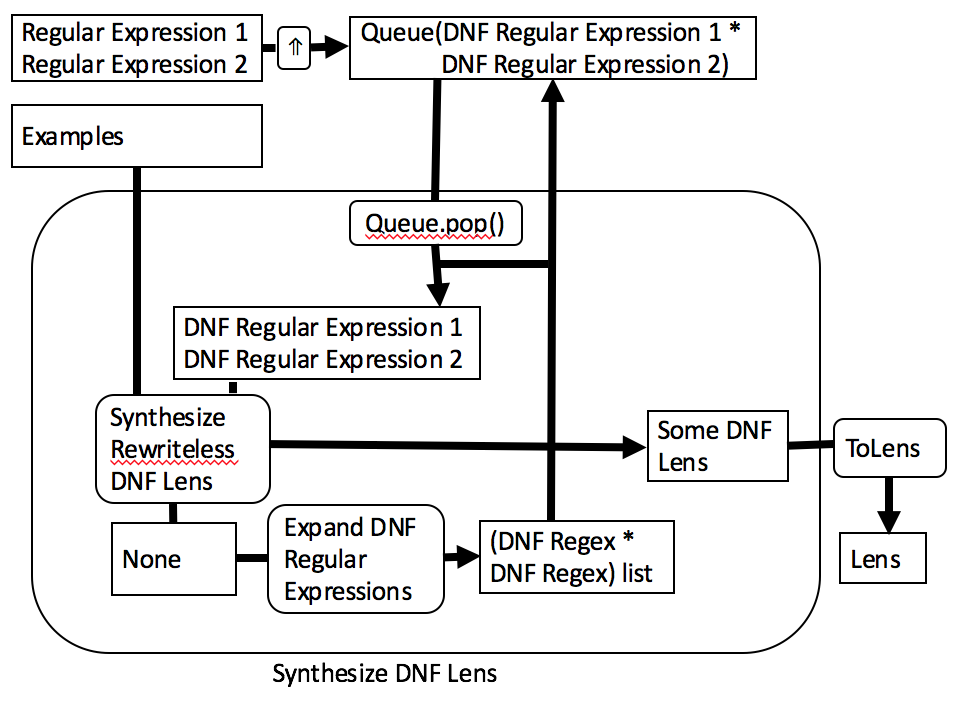
\includegraphics[scale=.5]{synth-lens-schematic.png}
\label{fig:synth-lens-schematic}
\end{figure}
The synthesis algorithm is shown in a schematic diagram in 
Figure~\ref{fig:synth-lens-schematic}.  The algorithm takes in a pair of
regular expressions, and examples, and converts the regular expressions into
DNF regular expressions, using $\ToDNFRegex{}$.
These then get enqueued, and SynthDNFLens, where the bulk of the work
occurs.

In SynthDNFLens, the highest priority DNF regular expression pair, $\DNFRegex$
and $\DNFRegexAlt$, is popped.
Then, SynthRewritelessDNF sees if there exists DNF lens $\DNFLens
\OfRewritelessType \DNFRegex \Leftrightarrow \DNFRegexAlt$ which satisfies the examples.
If none are found, then each rewrite is applied once on each side of the regular
expressions.
This new list of DNF regular expression doubles is enqueued, and SynthDNFLens is
called again.
If one is found, this DNF lens gets converted to a normal lens, and is returned
to the user.

\subsection{Priority Queue}
The priority queue is implemented using a naive list implementation.
We say that the lower the priority value, the higher the priority.
The priority value of an element is based on the number of expansions that have been
preformed, combined with the distance between the two regular expressions, based
on a psuedometric $\Distance$ we have implemented.  This pseudometric is implemented
as the sum of simpler pseudometrics,
$\Distance = \Distance_{size}+\Distance_{dist}$.

$\Distance_{size}$ is defined as merely the difference in the sizes of the DNF
regular expressions.
$\Distance_{size}(\DNFRegex,\DNFRegexAlt)=\AbsOf{\Size(\DNFRegex)-\Size(\DNFRegexAlt)}$

$\Distance_{dist}$ captures how different the distribution of
user defined regular expressions are from each other.
The distribution of user defined regular expressions can be viewed as an
infinite dimensional vector space over the reals, $\VectorSpace{}$.
The basis for this is $\SetOf{1*(\RegexVariable,n) | n\in\Nats, \RegexVariable
\text{ is a user defined regular expression}}$
DNF regular expressions with variables can map into this with a function by
counting the number of user defined data types present at a given level.
The formal definition for this mapping is given by the function \GetDist{}.

\begin{definition}\leavevmode\\
\label{def:getdist}
\begin{tabular}{@{}L@{}L@{}}
\GetDist(\DNFOf{\Sequence_1;\ldots;\Sequence_n}) &
=\GetDist(\Sequence_1)+\ldots+\GetDist(\Sequence_n)\\
\GetDist(\SequenceOf{\String_0;\Atom_1;\ldots;\Atom_n;\String_n}) &
=\GetDist(\Atom_1)+\ldots+\GetDist(\Atom_n)\\
\GetDist(\RegexVariable)&=1*(\RegexVariable,1)\\
\GetDist(\IterateLensOf{\DNFLens})&=\phi(\GetDist(\DNFLens))
\end{tabular}

where $\phi$ is the linear map sending $1*(\RegexVariable,n)$ to
$1*(\RegexVariable,n+1)$
\end{definition}

Using this, we now have a mapping from regular expressions into the distribution
of user defined regular exprssions.

$\Distance(\DNFRegex,\DNFRegexAlt)=\LOneNorm(\GetDist(\DNFRegex),\GetDist(\DNFRegexAlt))$
where $\LOneNorm$ is the taxicab metric on $\VectorSpace{}$.
The priority of a pair of DNF regular expressions, $(\DNFRegex{},\DNFRegexAlt{})$,
is $\Distance(\DNFRegex{},\DNFRegexAlt{})+8*expansion_{count}$.
Keeping track of expansion count is important as it allows for lower priority
expansions to be eventually popped, instead of getting stuck doing incorrect,
increasingly deep expansions whose DNF regular expressions have a low distance.
\afm{should i do an example, or is that going into too much detail?}
Experimentally, 8 was a good value for how much weight the expansion
count should get in the priority.  It allows for not getting stuck in a local
minima in the search space, while still allowing for the distance to choose the
correct expansion the majority of the time.

\subsection{SynthRewritelessDNF}
We find an efficient way to synthesize DNF lenses which do not use rewrites
through a clever encoding of the DNF regular expressions and examples.
A key insight into efficiently finding DNF lenses between two DNF regular
expressions is finding an ordering of DNF regular expressions which satisfy the
property such that, for two regular expressions $\DNFRegex$ and $\DNFRegexAlt$,
$\DNFRegex \leq \DNFRegexAlt$ and $\DNFRegexAlt \leq \DNFRegex$ if, and only if,
for some dnf lens $\DNFLens \OfType \DNFRegex \Leftrightarrow \DNFRegexAlt$,
with no use of \DNFRewriteLensRule{}.

ATTEMPT TO WRITE IT LESS FORMALLY

Unfortunately, while synthesizing a DNF regular expression, we must synthesize
two permutations, one to deal with determining which sequence
gets mapped to which (handling the commutativity of +), and one to deal
with determining within a sequence, which atoms get mapped to which
(handling swaps).

We found an incredibly efficient strategy for doing this, by further normalizing
the DNF regular expressions.  Instead of allowing any order of sequences, we
provide a total preorder on sequences, and order order the sequences
according to that ordering.

We do the same trick for normalizing the sequences.  While reordering a sequence
changes the semantics, we can temporarily reorder the sequence, remembering the
permutation of the reordering, and recover the original sequence later.

\begin{definition}
Given an ordering $\leq : A \rightarrow A \rightarrow \SetOf{-1,0,1}$,
we denote the dictionary ordering on lists of $As$, $\ListOf{\leq}$.
\end{definition}

\begin{definition}
  Given an ordering $\leq : A \rightarrow A \rightarrow \SetOf{-1,0,1}$,
  and $\ListOf{a_1;\ldots;a_n}\in \ListTypeOf{A}$
  We define $\SortingOf{\leq}{\ListOf{a_1;\ldots;a_n}}$ as
  $\sigma \in \PermutationSetOf{n}$ where if $i\leq j$,
  then $a_{\sigma(i)} \leq a_{\sigma(j)}$.

  We define $\SortOf{\leq}{\ListOf{a_1;\ldots;a_n}}$ as
  $\ListOf{a_{\sigma(1)};\ldots;a_{\sigma(n)}}$ where
  $\sigma=\SortingOf{\leq}{\ListOf{a_1;\ldots;a_n}}$
\end{definition}

\begin{definition}
  \begin{enumerate}
  \item
    $\DNFOf{\Sequence_1;\ldots\Sequence_n}
    \DNFLeq
    \DNFOf{\SequenceAlt_1;\ldots\SequenceAlt_m}$
    if
    $\SortOf{\SequenceLeq}{\ListOf{\Sequence_1;\ldots;\Sequence_n}}
    \ListOf{\SequenceLeq}
    \SortOf{\SequenceLeq}{[\SequenceAlt_1;\ldots;\SequenceAlt_n]}$.
    
  \item
    $\SequenceOf{\String_0;\Atom_1;\ldots;\Atom_n;\String_n}
    \SequenceLeq
    \SequenceOf{\StringAlt_0;\AtomAlt_1;\ldots;\AtomAlt_n;\String_n}$
    if
    $\SortOf{\AtomLeq}{\ListOf{\Atom_1\ldots\Atom_n}}
    \ListOf{\AtomLeq}
    \SortOf{\AtomLeq}{[\AtomAlt_1\ldots\AtomAlt_n]}$.

  \item
    $\StarOf{\DNFRegex} \AtomLeq \StarOf{\DNFRegexAlt}$
    if
    $\DNFRegex \DNFLeq \DNFRegexAlt$

  \item 
    $\DNFRegex \DNFEq \DNFRegexAlt$
    if
    $\DNFRegex \DNFLeq \DNFRegexAlt$ and $\DNFRegexAlt \DNFLeq \DNFRegex$.

  \item
    $\Sequence \SequenceEq \SequenceAlt$
    if
    $\Sequence \SequenceLeq \SequenceAlt$ and $\SequenceAlt \SequenceLeq
    \Sequence$.

  \item
    $\Atom \AtomEq \AtomAlt$
    if
    $\Atom \AtomLeq \AtomAlt$ and $\AtomAlt \AtomLeq \Atom$.
  \end{enumerate}
\end{definition}

This allows us to put our DNF regular expressions into a more normal form.

\begin{definition}
  \begin{enumerate}
  \item A DNF regular expression $\DNFOf{\Sequence_1;\ldots;\Sequence_n}$ is
    \textit{normalized} if $i \leq j$ implies $\Sequence_1\SequenceLeq\Sequence_j$,
    and each $\Sequence_i$ is normalized.
  \item A sequence $\SequenceOf{\Atom_1;\ldots;\Atom_n}$ is \textit{normalized}
    if $i \leq j$ implies $\Atom_i\AtomLeq\Atom_j$,
    and each $\Atom_i$ is normalized.
  \item An atom $\StarOf{\DNFRegex}$ is \textit{normalized} if
    $\DNFRegex$ is normalized.
  \end{enumerate}
\end{definition}

We can also easily normalize a DNF regular expression

\begin{definition}
  \begin{enumerate}
  \item $\NormalizeOf{\DNFOf{\Sequence_1;\ldots;\Sequence_n}} =
    \DNFOf{\NormalizeOf{\Sequence_{\sigma(1)}};\ldots;\NormalizeOf{\Sequence_{\sigma(n)}}}$,
    where
    $\sigma=\SortingOf{\SequenceLeq}
    {\ListOf{\NormalizeOf{\Sequence_1};\ldots;\NormalizeOf{\Sequence_n}}}$
  \item $\NormalizeOf{\SequenceOf{\String_0;\Atom_1;\ldots;\Atom_n;\String_n}} =
    \SequenceOf{\String_0;\Atom_{\sigma(1)};\ldots;\Atom_{\sigma(n)};\String_n}$,
    where
    $\sigma=\SortingOf{\AtomLeq}
    {\ListOf{\NormalizeOf{\Atom_1};\ldots;\NormalizeOf{\Atom_n}}}$
  \item $\NormalizeOf{\StarOf{\DNFRegex}}=\StarOf{\NormalizeOf{\DNFRegex}}$
  \end{enumerate}
\end{definition}

\begin{theorem}
  \begin{enumerate}
  \item
    If $\DNFOf{\Sequence_1;\ldots;\Sequence_n}$ and
    $\DNFOf{\SequenceAlt_1;\ldots;\SequenceAlt_m}$ are normalized, and
    $\DNFOf{\Sequence_1;\ldots;\Sequence_n}\DNFEq\DNFOf{\SequenceAlt_1;\ldots;\SequenceAlt_n}$
    then
    $n=m$ and
    $\Sequence_i = \SequenceAlt_i$ for all $i\in\RangeIncInc{1}{n}$
  \item
    If $\NormalizeOf{\SequenceOf{\Atom_1;\ldots;\Atom_n}} \DNFEq
    \NormalizeOf{\SequenceOf{\AtomAlt_1;\ldots;\AtomAlt_n}}$ then
    $\NormalizeOf{\Atom_{\sigma_1(i)}} =
    \NormalizeOf{\AtomAlt_{\sigma_2(i)}}$ for all $i$
    where $\sigma_1 =
    \SortingOf{\SequenceLeq}{\ListOf{\NormalizeOf{\Atom_1};\ldots;\NormalizeOf{\Atom_n}}}$
    and $\sigma_2 =
    \SortingOf{\DNFLeq}{\ListOf{\NormalizeOf{\AtomAlt_1};\ldots;\NormalizeOf{\AtomAlt_n}}}$
  \item
    tester
   % If $\NormalizeOf{\StarOf{\DNFRegex}}\DNFEq\NormalizeOf{\StarOf{\DNFRegexAlt}}$
  \end{enumerate}
\end{theorem}

\begin{definition}
  \begin{enumerate}
  \item
    Let
    $\DNFOf{\Sequence_1;\ldots;\Sequence_n}$
    and
    $\DNFOf{\SequenceAlt_1;\ldots;\SequenceAlt_n}$
    be two DNF regular expressions, where
    $\NormalizeOf{\DNFOf{\Sequence_1;\ldots;\Sequence_n}} \DNFEq
    \NormalizeOf{\DNFOf{\SequenceAlt_1;\ldots;\SequenceAlt_n}}$.
    $\DNFLensSynthOf{\DNFOf{\Sequence_1;\ldots;\Sequence_n}}
    {\DNFOf{\SequenceAlt_1;\ldots;\SequenceAlt_n}}=
    (\DNFLensOf{\SequenceLens_1;\ldots;\SequenceLens_n},\sigma)$
    where
    $\SequenceLens_i=\SequenceLensSynthOf{\Sequence_1}{\SequenceAlt_{\sigma(i)}}$
    and
    $\sigma=\SortingOf{\SequenceLeq}{\ListOf{\NormalizeOf{\Sequence_1};\ldots;\NormalizeOf{\Sequence_n}}}
    \Compose
    \SortingOf{\SequenceLeq}{\ListOf{\NormalizeOf{\SequenceAlt_1};\ldots;\NormalizeOf{\SequenceAlt_n}}}$
  \item
    Let
    $\SequenceOf{\String_0;\Atom_1;\ldots;\Atom_n;\String_n}$
    and
    $\SequenceOf{\StringAlt_0;\AtomAlt_1;\ldots;\AtomAlt_n;\StringAlt_n}$
    be two sequences, where
    $\NormalizeOf{\SequenceOf{\String_0;\Atom_1;\ldots;\Atom_n;\String_n}} \SequenceEq
    \NormalizeOf{\SequenceOf{\StringAlt_0;\AtomAlt_1;\ldots;\AtomAlt_n;\StringAlt_n}}$.
    $\SequenceLensSynthOf{\SequenceOf{\String_0;\Atom_1;\ldots;\Atom_n;\String_n}}
    {\SequenceOf{\StringAlt_0;\AtomAlt_1;\ldots;\AtomAlt_n;\StringAlt_n}}=
    (\SequenceLensOf{(\String_0,\StringAlt_0);\AtomLens_1;\ldots;\AtomLens_n;(\String_n,\StringAlt_n)},\sigma)$
    where
    $\AtomLens_i=\AtomLensSynthOf{\Atom_1}{\AtomAlt_{\sigma(i)}}$
    and
    $\sigma=\SortingOf{\AtomLeq}{\ListOf{\NormalizeOf{\Atom_1};\ldots;\NormalizeOf{\Atom_n}}}
    \Compose
    \SortingOf{\SequenceLeq}{\ListOf{\NormalizeOf{\AtomAlt_1};\ldots;\NormalizeOf{\AtomAlt_n}}}$
  \item
    Let
    $\StarOf{\DNFRegex}$
    and
    $\StarOf{\DNFRegexAlt}$
    be two atoms, where
    $\NormalizeOf{\StarOf{\DNFRegex}} \SequenceEq
    \NormalizeOf{\StarOf{\DNFRegexAlt}}$.
    $\AtomLensSynthOf{\StarOf{\DNFRegex}}
    {\StarOf{\DNFRegexAlt}}=
    \IterateLensOf{\DNFLensSynthOf{\DNFRegex}{\DNFRegexAlt}}$
  \end{enumerate}
\end{definition}

\begin{theorem}
  $\NormalizeOf{\DNFRegex}\DNFEq\NormalizeOf{\DNFRegexAlt}$
  if, and only
  if, there exists a $\DNFLens \OfType \DNFRegex \Leftrightarrow \DNFRegexAlt$,
  where the typing of $\DNFLens\OfType\DNFRegex\Leftrightarrow\DNFRegexAlt$
  has no applications of a rewrite rule.
\end{theorem}

Unfortunately, while this can find a well typed DNF lens, it doesn't
necessarily find the one that matches the examples.  In the situation where
there are multiple valid sorted orderings, there are multiple different lenses
with potentially different semantics.  Instead of iterating through all the
possible sortings, and finding one that matches the examples, we would like to
be able to immediately find only a sorting which satisfies the examples.

The key insight here is that certain invariants must hold for a DNF lens to have
semantics which match the examples.

\begin{enumerate}
\item If a source example string matches one of the clauses during parsing,
it must be sent to the clause the target example string matches during parsing.
\item If a source example string matches a user defined regular expression during
parsing, the target must match the exact same string during parsing.
\item If a source example string matches an iteration, then the target must iterate
the same number of times, and all the invariants must hold for each iterated part.
\end{enumerate}

This is done by joining additional parsing information alongside the regular
expression components, and creating an ordering on DNF Regular expressions
with parsing information.\afm{This would be a really in depth thing to describe,
worth going into?}
% end implementation


% begin evaluation
\section{Evaluation}
We ran our algorithm on tests validating our ability to handle regular
expression equivalences, tests derived from the Augeus test suite, and from
tests derived from the FlashFill tests.
The values presented are the arithmetic means of 10 test runs.
The tests were run on a 2.5 GHz Intel Core i7 processor, with
16 GB of 1600 MHz DDR3, running Mac OS X Yosemite.

\begin{figure*}
\centering
\begin{tabular}{|c|c|c|c|c|}
\hline
\bfseries Test & \bfseries ForceExpandTime & \bfseries ForceExpandExamplesRequired
& \bfseries Computation Time & \bfseries Examples Required
\csvreader[head to column names]{generated-data/data.csv}{}
{\\\hline\Test & \ForceExpandTime & \ForceExpandExamplesRequired & \ComputationTime & \ExamplesRequired}
\\\hline
\end{tabular}

\end{figure*}

\subsection{Speed}
Figure~\ref{fig:runtimes-table} provides the runtime of our algorithm on our
test suite.
In this figure, we want to minimize runtime, as a smaller runtime means we were
able to synthesize very efficiently.
We found that, on many of our difficult examples, our algorithm was able to find
the appropriate lens very quickly.

However, we can also see where the strengths and weaknesses are in our approach.
In particular, our synthesis strategy does quite well on problems that only
include a small number of transformations, even if the number of clauses is
decently large.
This is as expected, for after the appropriate transformations have been found,
the problem of finding the lens between the resulting DNF Regular Expressions
is merely as difficult as ordering the clauses.

For example, the address problem is the second slowest lens to synthesize.
This is because there is a large number of required expansions of user defined
data types, and there are multiple required star transformations.
Furthermore, there are a large number of potential star transformations because
of the large number of stars.
In addition to requiring a relatively deep search, this search is made much
more difficult because of the breadth of the search.
This shows us where our algorithm can hit issues.
When there are a large number of potential transformations, and there are a
large number of required transformations, our search gets more complicated,
and things slow down.

Another place where our synthesis algorithm preforms badly is where there is not
only a large number of clauses generated, but they also have a non-identity
lens between them.
For example, the double capitalization problem is another slowest test, despite
being an intuitively easy function to figure out, looking at it as a human.
This is because the algorithm problem has an exponential blow up in terms
of the number of clauses, when there are many regular expressions +d together.
If we take this problem to the logical extremes, we see that the the triple
capitalization problem takes 6.974 seconds, and the quadruple capitalization
problem takes 33 minutes and 54.730 seconds.

\subsection{Importance of Examples}
We wanted to see how many examples were required to synthesize the correct
bijective lens.
However, because of our implicit understanding of the algorithm, we fear we may
choose examples that we know will work well with the synthesis algorithm,
instead of choosing examples that users are likely to.
Because of that, we test the number of examples that it takes to generate the
correct lens, with randomly generated examples.


As we see in Figure~\ref{fig:examples-required-table}, examples are not too
important for synthesizing bijective lenses.\bcp{If that's really the
  conclusion, then maybe we should have written a paper about synthesizing
  bijective lenses {\em without\/} examples!  But I don't think we can
  actually conclude this from the examples we have.  }
Because bijective lenses have very few well typed programs, compared to the
number of functions, oftentimes just a few examples is sufficient.
As would be expected, the functions that have to make choices about the
locations of where data goes are those that require more examples.
In particular, the address problem requires more examples, because it must make
choices of where information goes, like which name is the a person's first name,
and which is their last.

\subsection{Importance of User Defined Data Types}

User defined data types are very critical to the algorithm and performance of
the synthesis algorithm.  User defined data types help direct the search of
which expansions should be performed.  Furthermore, they help to reduce the
number of clauses we have to deal with.  There is a potentially exponentially
large blowup in converting regular expressions into DNF form, but keeping
certain portions of the regular expressions abstracted lessens that blowup,
as those regular expressions are kept atomic in converting into DNF form.

User defined data types are also critical in the applications of previously
defined lenses.  We restrict the application of previously defined lenses to
only on user defined data types in the synthesis algorithm.  We then group the
user defined data types based on which have previously defined lenses between
them.  This allows for efficient recognition of when two user defined regular
expressions can be mapped to each other.  Removing the ability to use previously
defined lenses makes certain problems intractable, like (example1, example2,
example3).

While we can simulate the use of user defined data types automatically, by
giving regular expressions which have the same syntax the same user defined data
type, manually inputting them performs better in practice.  This is because the
procedure for automatically creating user defined data types creates far more
data types, which then creates a more complicated search problem.
% end evaluation

% begin discussion
\section{Discussion}

We found that in practice, requiring a user to put in more information for the
synthesis of a string transformation creates a more reliable algorithm.
However, this comes at a few costs.  The user needs to know how to write out
regular expressions.

The largest difficulty in this is the restriction to bijective lenses.
Oftentimes, we find the need to hide information away in some alternate form.
For example, there is oftentimes whitespace in the definition of a regular
expression.  This whitespace must be copied somehow over to the other side.
Oftentimes this requires the use of having a portion of the string dedicated to
holding the whitespace information of the other side.

Another annoyance is the fact that if the correct lens does not exist,
rarely does the tool terminate.  Much of the time it will just spin trying to
perform increasingly complicated transformations to find the correct lens.
A better solution would be to find something close to the correct lens, and have
a user interaction model that supports iterative synthesis.  The user could give
more examples which fix where the program is wrong.

\subsection{Future Work}
Some of the issues seen in this have already been observed.  For example, in the
quotient lens paper, the issue of having to hack a place in the source string to
move whitespace information from the view to the source was noted.  An extension
we would like to work on would be able to synthesize quotient lenses.

Another approach to having disparate information on each side of the lens is
through the use of symmetric lenses.  This could be another approach to the
whitespace problem. 
% end discussion


% begin related-work
\section{Related Work}
\subsection{FlashFill}
FlashFill is another string transformation program.  FlashFill takes input and
output examples as its only form of specification.  For FlashFill's primary use
case, providing easy transformations of Excel data, input and output examples as
the only specification makes a lot of sense.  Our tool is intended for use for
programmers to use, who already know regular expressions.  Our tool is oriented
towards a situation where a programmer would check the generated code into a
repository.  From requiring this extra information, our tool is able to handle
synthesize complicated functions that go beyond what FlashFill can synthesize.
For example, given 21 examples of extracting the first author, with the names
reversed, FlashFill still gave incorrect outputs for a number of inputs, even
when those inputs are a similar form to the provided examples.

Furthermore, even if FlashFill were to synthesize the correct program, it would
be foolhardy to check the generated code into a repository.  FlashFill does not
fail on inputs it doesn't know how to handle, rather it tries to provide an
output.  This is different from the generated lenses, which will quickly
fail on inputs that do not match it's intended specification.  Furthermore, the
specification of what inputs should be handled are provided by the user, not
inferred from the examples, giving it more reliability. \afm{talk about how it
  did on bibtex example, more specific on what it did wrong, maybe?}

\subsection{FlashExtract}
FlashExtract is a program that takes an input of a string, and a partial
labeling of substrings within that string, to try to label the rest of the
substrings.  FlashExtract was able to label some amounts of the strings, but was
unable to handle reorderings of the data well.  While it would do well in
extracting data when the data came in the same form, for example, when given a
Bibtex file where the fields come in a specific order, the data would do well,
however, FlashExtract was unable to handle when fields were given in different
orders, even if previous examples in that order were given.
% end related-work

% begin conclusion
\section{Conclusion}

We have coded up an implementation of type directed synthesis on a domain
specific language of bijective lenses.  This program allows users to input two
regular expressions, and a few input/output examples, and synthesizes a
bijective lens between those regular expressions, matching those input/output
examples.  While lenses are very useful for their guarantees, they are a
difficult domain specific language to code in, in practice.  This program
provides an easier interaction model for the creation of lenses through using
synthesis as the way to interact with the programmer.

This synthesis algorithm is competitive with state of the art tools for
synthesis on strings transformations.  This gain is made through requiring a
larger amount of user interaction with the synthesis algorithm.  However, in the
for this increased interaction, the program provides the capabilities of
synthesizing very complicated transformations, and provides stronger guarantees
about correctness on inputs dissimilar to those provided in the examples.
% end conclusion

\appendix

\ifanon\else
\acks 
%Expeditions in Computer Augmented Program Engineering (ExCAPE, NSF
%Award CCF-1138996).
%Acknowledgments, if needed.
\finish{Write me.  Mention all relevant grants, esp. DARPA.}
\fi

% We recommend abbrvnat bibliography style.

\bibliographystyle{abbrvnat}

% The bibliography should be embedded for final submission.

\bibliography{local}

% Appendices.

\onecolumn
% begin proofs
\section{Proofs}
%proof-dnfrc start
%First we will prove some lemmas.
\begin{lemma}[Equivalence of \ConcatSequence{} and \Concat{}]
If $\LanguageOf{\Regex}=\LanguageOf{\Sequence}$,
and $\LanguageOf{\RegexAlt}=\LanguageOf{\SequenceAlt}$,
then $\LanguageOf{\RegexConcat{\Regex}{\RegexAlt}}=\LanguageOf{\ConcatSequenceOf{\Sequence}{\SequenceAlt}}$.
\end{lemma}
\begin{proof}
Let $\Sequence=\SequenceOf{\String_0\SequenceSep\Atom_1\SequenceSep\ldots
\SequenceSep\Atom_n\SequenceSep\String_n}$, and
let\\ $\SequenceAlt=[\StringAlt_0\SequenceSep\AtomAlt_1\SequenceSep\ldots
\SequenceSep\AtomAlt_m\SequenceSep\StringAlt_m]$\\
\begin{tabular}{@{}L@{}L@{}}
\LanguageOf{\ConcatSequenceOf{\Sequence}{\SequenceAlt}} & = 
\LanguageOf{\SequenceOf{\String_0\SequenceSep\Atom_1\SequenceSep\ldots
\SequenceSep\Atom_n\SequenceSep\String_n\Concat\StringAlt_0\SequenceSep{}
\AtomAlt_1\SequenceSep\ldots\SequenceSep\AtomAlt_m\SequenceSep\StringAlt_m}} \\
& = 
\{\String_0\Concat\String_1'\Concat\ldots\Concat\String_n'\Concat\String_n
\Concat\StringAlt_0\Concat\StringAlt_1'\Concat\ldots
\Concat\StringAlt_m'\Concat\StringAlt_m \\
& \hspace{5em} \SuchThat{} \String_i'\in\LanguageOf{\Atom_i} \BooleanAnd{}
\StringAlt_i'\in\LanguageOf{\AtomAlt_i}\}\\
& = 
\{\String\Concat\StringAlt{} \SuchThat{} \String\in\LanguageOf{\Sequence}
\BooleanAnd{} \StringAlt\in\LanguageOf{\SequenceAlt}\}\\
& =
\{\String\Concat\StringAlt{} \SuchThat{} \String\in\LanguageOf{\Regex}
\BooleanAnd{} \StringAlt\in\LanguageOf{\RegexAlt}\}\\
& =
\LanguageOf{\RegexConcat{\Regex}{\RegexAlt}}
\end{tabular}
\end{proof}

\begin{lemma}[Equivalence of \ConcatDNF{} and \Concat{}]
\label{lem:cdnfeq}
If $\LanguageOf{\Regex}=\LanguageOf{\DNFRegex}$,
and $\LanguageOf{\RegexAlt}=\LanguageOf{\DNFRegexAlt}$,
then $\LanguageOf{\RegexConcat{\Regex}{\RegexAlt}}=
\LanguageOf{\ConcatDNFOf{\DNFRegex}{\DNFRegexAlt}}$.
\end{lemma}
\begin{proof}
Let $\DNFRegex=\DNFOf{\Sequence_0\DNFSep\ldots\DNFSep\Sequence_n}$, and
let $\DNFRegexAlt=\DNFOf{\SequenceAlt_0\DNFSep\ldots\DNFSep\SequenceAlt_m}$
\begin{tabular}{@{}L@{}L@{}}
\LanguageOf{\ConcatDNFOf{\DNFRegex}{\DNFRegexAlt}} & = 
\LanguageOf{\DNFOf{\ConcatSequenceOf{\Sequence_i}{\SequenceAlt_j}
\text{ for $i\in\RangeIncInc{1}{n}$, $j\in\RangeIncInc{1}{m}$}}} \\
& = 
\{\String\SuchThat \String\in\ConcatSequenceOf{\Sequence_i}{\SequenceAlt_j}\\
& \hspace{5em}
\text{ where $i\in\RangeIncInc{1}{n}$, $j\in\RangeIncInc{1}{m}$}\}\\
& = 
\{\String\Concat\StringAlt{} \SuchThat{} \String\in\LanguageOf{\Sequence_i}
\BooleanAnd{} \StringAlt\in\LanguageOf{\SequenceAlt_j}\}\\
& \hspace{5em}
\text{ where $i\in\RangeIncInc{1}{n}$, $j\in\RangeIncInc{1}{m}$}\}\\
& =
\{\String\Concat\StringAlt{} \SuchThat{} \String\in\LanguageOf{\DNFRegex}
\BooleanAnd{} \StringAlt\in\LanguageOf{\DNFRegexAlt}\}\\
& =
\{\String\Concat\StringAlt{} \SuchThat{} \String\in\LanguageOf{\Regex}
\BooleanAnd{} \StringAlt\in\LanguageOf{\RegexAlt}\}\\
& =
\LanguageOf{\RegexConcat{\Regex}{\RegexAlt}}
\end{tabular}
\end{proof}

\begin{lemma}[Equivalence of \OrDNF{} and \Or{}]
\label{lem:odnfeq}
If $\LanguageOf{\Regex}=\LanguageOf{\DNFRegex}$,
and $\LanguageOf{\RegexAlt}=\LanguageOf{\DNFRegexAlt}$,
then $\LanguageOf{\RegexOr{\Regex}{\RegexAlt}}=
\LanguageOf{\OrDNFOf{\DNFRegex}{\DNFRegexAlt}}$.
\end{lemma}
\begin{proof}
Let $\DNFRegex=\DNFOf{\Sequence_0\DNFSep\ldots\DNFSep\Sequence_n}$, and
let $\DNFRegexAlt=\DNFOf{\SequenceAlt_0\DNFSep\ldots\DNFSep\SequenceAlt_m}$
\begin{tabular}{@{}L@{}L@{}}
\LanguageOf{\OrDNFOf{\DNFRegex}{\DNFRegexAlt}} & = 
\LanguageOf{\DNFOf{\Sequence_0\DNFSep\ldots\DNFSep\Sequence_n\DNFSep
\SequenceAlt_1\DNFSep\ldots\DNFSep\SequenceAlt_m}}\\
& = 
\{\String\SuchThat{} \String\in\Sequence_i\vee\String\in\SequenceAlt_j\\
& \hspace{5em}
\text{ where $i\in\RangeIncInc{1}{n}$, $j\in\RangeIncInc{1}{m}$}\}\\
& = 
\{\String{} \SuchThat{} \String\in\LanguageOf{\DNFRegex}
\BooleanOr{} \String\in\LanguageOf{\DNFRegexAlt}\}\\
& =
\{\String \SuchThat{} \String\in\LanguageOf{\Regex}
\BooleanOr{} \String\in\LanguageOf{\RegexAlt}\}\\
& =
\LanguageOf{\RegexOr{\Regex}{\RegexAlt}}
\end{tabular}\\
\end{proof}

\dnfrc*
\begin{proof}
By structural induction.

Let $\Regex=\String$.
$\LanguageOf{\ToDNFRegex(\String)}=\LanguageOf{\DNFOf{\SequenceOf{\String}}}=
\{\String\}=\LanguageOf{\String}$

Let $\Regex=\emptyset$.
$\LanguageOf{\ToDNFRegex(\emptyset)}=\LanguageOf{\DNFOf{}} =
\{\} = \LanguageOf{\emptyset}$.

Let $\Regex=\StarOf{\Regex'}$.
By induction assumption, $\LanguageOf{\ToDNFRegex(\Regex')}=
\LanguageOf{\Regex'}$.\\
\begin{tabular}{@{}L@{}L@{}}
\LanguageOf{\ToDNFRegex(\StarOf{\DNFRegex'})} & =
\LanguageOf{\DNFOf{\SequenceOf{\StarOf{\ToDNFRegex(\Regex')}}}}\\
& =
\{\String\SuchThat\String\in
\LanguageOf{\SequenceOf{\StarOf{\ToDNFRegex(\Regex')}}}\}\\
& = 
\{\String\SuchThat{} \String\in\LanguageOf{\StarOf{\ToDNFRegex(\Regex')}}\}\\
& =
\{\String_1\Concat\ldots\Concat\String_n\SuchThat{}
n\in\Nats\\
& \hspace*{3em}\BooleanAnd\String_i\in\LanguageOf{\ToDNFRegex(\Regex')}\}\\
& =
\{\String_1\Concat\ldots\Concat\String_n\SuchThat{}
n\in\Nats\BooleanAnd\String_i\in\LanguageOf{\Regex'}\}\\
& = \LanguageOf{\StarOf{\Regex'}}
\end{tabular}

Let $\Regex=\RegexConcat{\Regex_1}{\Regex_2}$.
By induction assumption,
$\LanguageOf{\ToDNFRegex(\Regex_1)}=\LanguageOf{\Regex_1}$, and
$\LanguageOf{\ToDNFRegex(\Regex_2)}=\LanguageOf{\Regex_2}$.
$\ToDNFRegex(\RegexConcat{\Regex_1}{\Regex_2})=
\ConcatDNFOf{\ToDNFRegex(\Regex_1)}{\ToDNFRegex(\Regex_2)}$.
By Lemma~\ref{lem:cdnfeq},
$\RegexConcat{\Regex_1}{\Regex_2}=
\ConcatDNFOf{\ToDNFRegex(\Regex_1)}{\ToDNFRegex(\Regex_2)}$.

Let $\Regex=\RegexOr{\Regex_1}{\Regex_2}$.
By induction assumption,
$\LanguageOf{\ToDNFRegex(\Regex_1)}=\LanguageOf{\Regex_1}$, and
$\LanguageOf{\ToDNFRegex(\Regex_2)}=\LanguageOf{\Regex_2}$.
$\ToDNFRegex(\RegexOr{\Regex_1}{\Regex_2})=
\OrDNFOf{\ToDNFRegex(\Regex_1)}{\ToDNFRegex(\Regex_2)}$.
By Lemma~\ref{lem:odnfeq},
$\RegexOr{\Regex_1}{\Regex_2}=
\OrDNFOf{\ToDNFRegex(\Regex_1)}{\ToDNFRegex(\Regex_2)}$.
\end{proof}
%proof-dnfrc end



%proof-dnfrs start
%First we will prove some lemmas.
\begin{lemma}
\label{lem:sequence-rx}
Let $\SequenceOf{\String_0\SequenceSep\Atom_1\SequenceSep
\ldots\Atom_n\SequenceSep\String_n}$ be a sequence,
and\\
$\ToDNFRegex(\ToRegex(\Atom_i))=\DNFOf{\SequenceOf{\Atom_i}}$.
Then,\\$\ToDNFRegex(\ToRegex(\SequenceOf{\String_0\SequenceSep\Atom_1\SequenceSep
\ldots\Atom_n\SequenceSep\String_n}))=$\\
$\DNFOf{\SequenceOf{\String_0\SequenceSep\Atom_1\SequenceSep
\ldots\Atom_n\SequenceSep\String_n}}$.
\end{lemma}
\begin{proof}
By induction on $n$.

Let $n=0$.
$\Sequence=\SequenceOf{\String_0}$.\\
$\ToDNFRegex(\ToRegex(\SequenceOf{\String_0}))=
\ToDNFRegex(\String_0)=\DNFOf{\SequenceOf{\String_0}}$

Let $n>0$,
$\Sequence=\SequenceOf{\String_0\SequenceSep\Atom_1\SequenceSep
\ldots\Atom_n\SequenceSep\String_n}$.\\
$\ToDNFRegex(\ToRegex(\SequenceOf{\String_0\SequenceSep\Atom_1\SequenceSep
\ldots\Atom_n\SequenceSep\String_n}))$\\
$\ToDNFRegex(\ToRegex(\SequenceOf{\String_0\SequenceSep\Atom_1\SequenceSep
\ldots\Atom_{n-1}\SequenceSep\String_{n-1}})\Concat\ToRegex(\Atom_n)
\Concat\String_n)$=\\
$\ToDNFRegex(\ToRegex(\SequenceOf{\String_0\SequenceSep\Atom_1\SequenceSep
\ldots\Atom_{n-1}\SequenceSep\String_{n-1}}))
\ConcatDNF\\
\ToDNFRegex(\ToRegex(\Atom_n))
\ConcatDNF\\
\ToDNFRegex(\String_{n-1})$=
$\DNFOf{\SequenceOf{\String_0\SequenceSep\Atom_1\SequenceSep
\ldots\Atom_{n-1}\SequenceSep\String_{n-1}}}
\ConcatDNF\\
\DNFOf{\SequenceOf{\Atom_n}}
\ConcatDNF
\DNFOf{\SequenceOf{\String_n}}$=
$\DNFOf{\SequenceOf{\String_0\SequenceSep\Atom_1\SequenceSep
\ldots\Atom_n\SequenceSep\String_n}}$.
\end{proof}



\begin{lemma}
\label{lem:dnf-rx}
Let $\DNFOf{\Sequence_1\DNFSep\ldots\DNFSep\Sequence_n}$ be a sequence,
and\\ $\ToDNFRegex(\ToRegex(\Sequence_i))=\DNFOf{\Sequence_i}$.
Then,\\ $\ToDNFRegex(\ToRegex(\DNFOf{\Sequence_1\DNFSep\ldots\DNFSep\Sequence_n}))=
\DNFOf{\Sequence_1\DNFSep\ldots\DNFSep\Sequence_n}$.
\end{lemma}
\begin{proof}

By induction on $n$.

Let $n=0$
$\ToDNFRegex(\ToRegex(\DNFOf{}))=\ToDNFRegex(\emptyset)=\DNFOf{}$.

Let $n>0$
$\ToDNFRegex(\ToRegex(\DNFOf{\Sequence_1\SequenceSep\ldots\SequenceSep\Sequence_n}))=
\ToDNFRegex(\ToRegex(\DNFOf{\Sequence_1\SequenceSep\ldots\SequenceSep\Sequence_{n-1}})
\Concat\ToRegex(\Sequence_n))$=
$\ToDNFRegex(\ToRegex(\DNFOf{\Sequence_1\SequenceSep\ldots\SequenceSep\Sequence_{n-1}}))
\ConcatDNF\\\ToDNFRegex(\ToRegex(\Sequence_n))$=
$\DNFOf{\Sequence_1\SequenceSep\ldots\SequenceSep\Sequence_n}$
\end{proof}

\begin{lemma}[Elimination of $\ToDNFRegex\Compose\ToRegex$]\leavevmode
\begin{enumerate}
\item $\ToDNFRegex(\ToRegex(\Atom))=\DNFOf{\SequenceOf{\Atom}}$
\item $\ToDNFRegex(\ToRegex(\Sequence))=\DNFOf{\Sequence}$
\item $\ToDNFRegex(\ToRegex(\DNFRegex))=\DNFRegex$
\end{enumerate}
\end{lemma}
\begin{proof}
By mutual induction

Let $\StarOf{\DNFRegex}$ be an atom.
$\ToDNFRegex(\ToRegex(\StarOf{\DNFRegex}))=
\ToDNFRegex(\StarOf{\ToRegex(\DNFRegex)})=
\DNFOf{\SequenceOf{\StarOf{\ToDNFRegex(\ToRegex(\DNFRegex))}}}=
\DNFOf{\SequenceOf{\StarOf{\DNFRegex}}}$

Let $\SequenceOf{\String_0\SequenceSep\Atom_1\SequenceSep\ldots
\SequenceSep\Atom_n\SequenceSep\String_n}$ be a sequence.
$\ToDNFRegex(\ToRegex(\SequenceOf{\String_0\SequenceSep\Atom_1\SequenceSep\ldots
\SequenceSep\Atom_n\SequenceSep\String_n}))$.
By induction assumption, for each $\Atom_i$,
$\ToDNFRegex(\ToRegex(\Atom_i))=\DNFOf{\SequenceOf{\Atom_i}}$.
By Lemma~\ref{lem:sequence-rx},
$\ToDNFRegex(\ToRegex(\SequenceOf{\String_0\SequenceSep\Atom_1\SequenceSep\ldots
\SequenceSep\Atom_n\SequenceSep\String_n}))=
\DNFOf{\SequenceOf{\String_0\SequenceSep\Atom_1\SequenceSep\ldots
\SequenceSep\Atom_n\SequenceSep\String_n}}$.

Let $\DNFOf{\Sequence_1\SequenceSep\ldots\SequenceSep\Sequence_n}$ be a DNF
regular expression.
By induction assumption, for each $\Sequence_i$,
$\ToDNFRegex(\ToRegex(\Sequence_i))=\DNFOf{\Sequence_i}$.
By Lemma~\ref{lem:dnf-rx},
$\ToDNFRegex(\ToRegex(\DNFOf{\Sequence_1\SequenceSep\ldots\SequenceSep\Sequence_n}))=
\DNFOf{\Sequence_1\SequenceSep\ldots\SequenceSep\Sequence_n}$.

\end{proof}
%proof-dnfrs end




%proof-dnfls start
%We will prove a couple of lemmas first.

\begin{lemma}[Expressibility of Safe Boilerplate Alterations]
\label{lem:boilerplate-alterations}
Suppose
\begin{enumerate}
\item $\UnambigConcat\SequenceOf{\String_0;\Atom_1;\ldots;\Atom_n;\String_n}$
\item $\UnambigConcat\SequenceOf{\StringAlt_0;\Atom_1;\ldots;\Atom_n;\StringAlt_n}$
\end{enumerate}
Then there exists a lens
$\Lens \OfType \Regex \Leftrightarrow \RegexAlt$ such that
\begin{enumerate}
\item $\Regex = \ToRegex(\SequenceOf{\String_0;\Atom_1;\ldots;\Atom_n;\String_n})$
\item $\RegexAlt = \ToRegex(\SequenceOf{\StringAlt_0;\Atom_1;\ldots;\Atom_n;\StringAlt_n})$
\item $\SemanticsOf{\Lens}=\SetOf{(\String,\StringAlt)\SuchThat
\String=\String_0\Concat\String_1'\Concat\ldots\Concat\String_n'\Concat\String_n
\BooleanAnd\\
\hspace*{6.1em}\StringAlt=\StringAlt_0\Concat\String_1'\Concat\ldots\Concat\String_n'\Concat\StringAlt_n
\BooleanAnd\\
\hspace*{6.1em}\String_i\in\LanguageOf{\Atom_i}}$
\end{enumerate}
\end{lemma}
\begin{proof}
By induction on $n$.

Let $n=0$.
Consider the Lens
\begin{mathpar}
\inferrule*
{
}
{
\ConstLensOf{\String_0}{\StringAlt_0} \OfType \String_0 \Leftrightarrow \StringAlt_0
}
\end{mathpar}
By inspection, this satisfies the desired properties.

Let $n>0$.
By induction, there exists a lens $\Lens \OfType \Regex \Leftrightarrow \RegexAlt$
satisfying the desired properties.
Consider the lens
\begin{mathpar}
\inferrule*[left=\Derivation]
{
\inferrule*
{
\inferrule*[vdots=1.5em]
{
}
{
}
}
{
\Lens \OfType \Regex \Leftrightarrow \RegexAlt
}\\
\inferrule*
{
}
{
\ConstLensOf{\String_n}{\StringAlt_n} \OfType \String_n \Leftrightarrow \StringAlt_n
}
}
{
\ConcatLensOf{\Lens}{\ConstLensOf{\String_n}{\StringAlt_n}}
\OfType
\Regex \Concat \String_n \Leftrightarrow
\RegexAlt \Concat \StringAlt_n
}

\inferrule*
{
\Derivation\\
\IdentityLensOf{\ToRegex(\Atom_n)} \OfType \ToRegex(\Atom_n) \Leftrightarrow \ToRegex(\Atom_n)
}
{
\ConcatLensOf{\ConcatLensOf{\Lens}{\ConstLensOf{\String_n}{\StringAlt_n}}}{\IdentityLensOf{\ToRegex(\Atom_n)}}
\OfType\\
\Regex \Concat \String_n \Concat \ToRegex(\Atom_n) \Leftrightarrow
\Regex \Concat \StringAlt_n \Concat \ToRegex(\Atom_n)
}
\end{mathpar}
By inspection, this satisfies the desired properties.
\end{proof}

\begin{lemma}[Creation of Lens from Identity Perm Sequence Lens]
\label{lem:id-clause}
Suppose
\begin{enumerate}
\item $\Sequence=\SequenceOf{\String_0 ; \Atom_1 ; \ldots ; \Atom_n; \String_n}$
\item $\SequenceAlt=\SequenceOf{\StringAlt_0 ; \AtomAlt_1 ; \ldots ; \AtomAlt_n ; \StringAlt_n}$
\item $(\SequenceLensOf{(\String_0,\StringAlt_0);\AtomLens_1 ; \ldots ;
	\AtomLens_n;(\String_n,\StringAlt_n)},id) \OfType
	\Sequence \Leftrightarrow \SequenceAlt$
\item For each $\AtomLens_i \OfType \Atom_i \Leftrightarrow \AtomAlt_i$,
there exists a $\Lens_i \OfType \ToRegex(\Atom_i) \Leftrightarrow
\ToRegex(\AtomAlt_i)$ such that $\SemanticsOf{\Lens_i}=\SemanticsOf{\AtomLens_i}$
\end{enumerate}
then there exists a $\Lens \OfType \ToRegex(\Sequence) \Leftrightarrow \ToRegex(\DNFRegexAlt)$ such that
$\SemanticsOf{\Lens} =
\SemanticsOf{(\SequenceLensOf{(\String_0,\StringAlt_0);\AtomLens_1 ; \ldots ; \AtomLens_n;(\String_n,\StringAlt_n)},id)}$.
\begin{proof}
By induction on $n$.

Let $n=0$, $(\SequenceLensOf{(\String_0,\StringAlt_0)},id) \OfType
\SequenceOf{\String_0} \Leftrightarrow \SequenceOf{\StringAlt_0}$.
Then consider
\begin{mathpar}
\inferrule[]
{
}
{
\ConstLensOf{\String_0}{\StringAlt_0}\OfType\String_0\Leftrightarrow\StringAlt_0
}
\end{mathpar}

$\String_0=\ToRegex(\SequenceOf{\String_0})$,
and
$\StringAlt_0=\ToRegex(\SequenceOf{\StringAlt_0})$.
$\SemanticsOf{\ConstLensOf{\String_0}{\StringAlt_0}}=
\SetOf{\String_0,\StringAlt_0}=
\SemanticsOf{\SequenceOf{(\String_0,\StringAlt_0)},id)}$.

Let $n>0$.
Let $\Sequence'=\SequenceOf{\String_0\SequenceSep\Atom_1\SequenceSep
\ldots\SequenceSep\Atom_{n-1}\SequenceSep\String_{n-1}}$,
and $\SequenceAlt'=\SequenceOf{\StringAlt_0\SequenceSep\AtomAlt_1\SequenceSep
\ldots\SequenceSep\AtomAlt_{n-1}\SequenceSep\StringAlt_{n-1}}$
By induction assumption, there exists a typing derivation
\begin{mathpar}
\inferrule*
{
\inferrule*[vdots=1.5em]
{
}
{
}
}
{
\Lens\OfType\ToRegex(\Sequence')\Leftrightarrow\ToRegex(\SequenceAlt')
}
\end{mathpar}
satisfying $\SemanticsOf{\Lens}=\\
\SemanticsOf{(\SequenceLensOf{(\String_0,\StringAlt_0);\AtomLens_1 ;
\ldots ; \AtomLens_{n-1};(\String_{n-1},\StringAlt_{n-1})},id)}$

By problem statement, there exists a typing derivation
\begin{mathpar}
\inferrule*[left=$\Derivation_n$]
{
\inferrule*[vdots=1.5em]
{
}
{
}
}
{
\Lens_{\AtomLens_{n}} \OfType
\ToRegex(\Atom_{n}) \Leftrightarrow \ToRegex(\AtomAlt_{n})
}
\end{mathpar}
satisfying $\SemanticsOf{\Lens_{\Atom_n}}
=\SemanticsOf{\Atom_n}$.

Consider the following lens typing
\begin{mathpar}
\inferrule*[left=\Derivation{}]
{
\Derivation_n\\
\inferrule*
{
}
{
\ConstLensOf{\String_n}{\StringAlt_n}
\OfType
\String_n \Leftrightarrow \StringAlt_n
}
}
{
\ConcatLensOf{\Lens_{\AtomLens_n}}{\ConstLensOf{\String_n}{\StringAlt_n}}
\OfType
\ToRegex(\Atom_n)\Concat\String_n \Leftrightarrow
\ToRegex(\AtomAlt_n)\Concat\StringAlt_n
}

\inferrule*{
\inferrule*
{
\inferrule*[vdots=1.5em]
{
}
{
}
}
{
\Lens\OfType\ToRegex(\Sequence) \Leftrightarrow \ToRegex(\SequenceAlt)
}\\
\Derivation{}
}
{
\ConcatLensOf
{\Lens}
{\ConcatLensOf{\Lens_{\AtomLens_n}}{\ConstLensOf{\String_n}{\StringAlt_n}}}
\OfType\\
\ToRegex(\Sequence)\Concat\ToRegex(\Atom_n)\Concat\String_n \Leftrightarrow
\ToRegex(\SequenceAlt)\Concat\ToRegex(\AtomAlt_n)\Concat\StringAlt_n
}
\end{mathpar}

\SemanticsOf{\ConcatLensOf
{\Lens}
{\ConcatLensOf{\Lens_{\AtomLens_n}}{\ConstLensOf{\String_n}{\StringAlt_n}}}}\\
\hspace*{3em}=\SetOf{(\String,\StringAlt)
\SuchThat
\String = \String'\Concat\String''\Concat\String_n\BooleanAnd
\StringAlt = \StringAlt'\Concat\StringAlt''\Concat\StringAlt_n\BooleanAnd\\
\hspace*{7em}
(\String',\StringAlt')\in\SemanticsOf{\Lens}\BooleanAnd
(\String'',\StringAlt'')\in\SemanticsOf{\Lens_{\AtomLens_n}}}\\
\hspace*{3em}=\SetOf{
(\String,\StringAlt)\SuchThat
\String=
\String_0\Concat\String_0'\Concat\ldots
\Concat\String_{n-1}'\Concat\String_{n-1}
\Concat \String_n \Concat \String_n'\BooleanAnd\\
\hspace*{7em}\StringAlt=\StringAlt_0\Concat\StringAlt_0'\Concat\ldots
\Concat\StringAlt_{n-1}'\Concat\StringAlt_{n-1}
\Concat \StringAlt_n \Concat \StringAlt_n'\BooleanAnd\\
\hspace*{7em}\String_i'\in\Atom_i\BooleanAnd\StringAlt_i'\in\AtomAlt_i}\\
\hspace*{3em}=\SemanticsOf{(\SequenceLensOf{(\String_0,\StringAlt_0);\AtomLens_1 ;
\ldots ; \AtomLens_n;(\String_n,\StringAlt_{n-1})},id)}
\end{proof}
\end{lemma}

\begin{theorem}[Unambiguity of $\Sep$]
Let $\Alphabet$ be an alphabet.  Let $\Alphabet_{\Sep}=\Alphabet\Union\SetOf{\Sep}$,
where \Sep{} is a character not in \Alphabet{}.
If $\Language_1, \ldots,
\Language_n$, are languages in $\StarOf{\Alphabet}$, then
$\UnambigConcat\SequenceOf{\LanguageOf{\Sep};\Language_1;\LanguageOf{\Sep};
\ldots;\LanguageOf{\Sep};\Language_n;\LanguageOf{\Sep}}$.
\end{theorem}
\begin{proof}
We prove this by induction on $n$.

Let $n=0$.  $\UnambigConcat\SequenceOf{\LanguageOf{\Sep}}$, as
$\UnambigConcat\SequenceOf{\Language}$, for any language $\Language$.

Let $n>0$.
Let $\String_i, \StringAlt_i\in\Language_i$ for all $i\in\RangeIncInc{1}{n}$,
and let $\Sep\String_1\Sep\ldots\Sep\String_n\Sep=\Sep\StringAlt_1\Sep\ldots\Sep\StringAlt_n\Sep$.
We want to show that $\String_n\Sep=\StringAlt_n\Sep$.
If they were not equal, then one string is strictly contained in the other, say without
loss of generality $\String_n\Sep$ is strictly contained in $\StringAlt_n\Sep$.
Because of that $\Sep\String_n\Sep$ is contained in $\StringAlt_n\Sep$, so $\Sep$
is contained in $\StringAlt_n\in\StarOf{\Sigma}$.  This is a contradiction,
as $\Sep\notin\Sigma$, so we know $\String_n\Sep=\StringAlt_n\Sep$, and so $\String_n=\StringAlt_n$.
This means that
$\Sep\String_0\Sep\ldots\Sep\String_{n-1}\Sep=\Sep\StringAlt_0\Sep\ldots\Sep\StringAlt_{n-1}$,
so by induction, I know $\String_i=\StringAlt_i$ for all $i$.
\end{proof}

\begin{definition}[Adjacent Swapping Permutation]
Let $\sigma_{i} \in S_n$ be the permutation where
$\sigma_{i}(i) = i+1$, $\sigma_{i}(i+1) = i$, $\sigma_{i}(k) = k$
when $k\neq i$, and $k\neq i+1$.
\end{definition}

\begin{lemma}[Expressibility of Adjacent Swapping Permutation Lens]
\label{lem:adj-perm-exp}
Suppose
\begin{enumerate}
\item $\sigma_i$ is an adjacent element swapping permutation
\item $\SequenceOf{\Sep;\Atom_1;\Sep\ldots\Sep;\Atom_n;\Sep}$ is a sequence with
all base strings equal to $\Sep$.
\end{enumerate}
Then there exists a typing of a lens $\Lens \OfType \Regex \Leftrightarrow \RegexAlt$ such that
\begin{enumerate}
\item $\LanguageOf{\Regex}=\LanguageOf{[\Sep;\Atom_1;\ldots;\Atom_n;\Sep]}$
\item $\LanguageOf{\RegexAlt}=\LanguageOf{[\Sep;\Atom_{\sigma_i(1)};\ldots;\Atom_{\sigma_i(n)};\Sep]}$
\item $\SemanticsOf{\Lens}=
\SetOf{(\String,\StringAlt)\SuchThat\String=\Sep\Concat\String_1\Concat\Sep\Concat\ldots\Concat\Sep\Concat\String_n\Concat\Sep
\BooleanAnd\\
\hspace*{6em}\StringAlt=\Sep\Concat\String_{\sigma_i(1)}\Concat\Sep\Concat\ldots\Concat\Sep\Concat\String_{\sigma_i(n)}\Sep\BooleanAnd\\
\hspace*{6em}\String_i\in\LanguageOf{\Atom_i}}$
\end{enumerate}
\begin{proof}
By the soundness of regular expressions, define regular expressions
$\Regex_1, \Regex_2, \Regex_3, \Regex_4$ as
$\Regex_1=\ToRegex([\Sep;\Atom_1;\ldots;\Atom_{i-1};\Sep])$,
$\Regex_2=\ToRegex(\Atom_i)$,
$\Regex_3=\ToRegex(\Atom_{i+1})$, and
$\Regex_4=\ToRegex([\Sep;\Atom_{i+1};\ldots;\Atom_{n};\Sep])$.
Consider the following deduction\bcp{I find these deductions a bit heavy and
  hard to read, but I guess I can get used to them.  }
\afm{Anybody have suggestions for better deduction package?}
\begin{mathpar}

\inferrule*[left=\Derivation{}]
{
\inferrule*
{
}
{
\IdentityLensOf{\Sep} \OfType \Sep \Leftrightarrow \Sep
}
\inferrule*
{
}
{
\IdentityLensOf{\Regex_3} \OfType \Regex_3 \Leftrightarrow \Regex_3
}
}
{
\SwapLensOf{\IdentityLensOf{\Sep}}{\IdentityLensOf{\Regex_3}} \OfType 
\Sep\Concat\Regex_3 \Leftrightarrow \Regex_3\Concat\String_i
}

\inferrule*[left=\Derivation{}']
{
\inferrule*
{
}
{
\IdentityLensOf{\Regex_2} \OfType \Regex_2 \Leftrightarrow \Regex_2
}\\
\Derivation
}
{
\SwapLensOf{\IdentityLensOf{\Regex_2}}{\SwapLensShortOf{\IdentityLensShortOf{\Sep}}{\IdentityLensShortOf{\Regex_3}}} \OfType
\Regex_2\Concat\Sep\Concat\Regex_3 \Leftrightarrow \Regex_3\Concat\Sep\Concat\Regex_2
}

\inferrule*[left=\Derivation{}'']
{
\inferrule*
{
}
{
\IdentityLensOf{\Regex_1} \OfType \Regex_1 \Leftrightarrow \Regex_1
}\\
\Derivation{}'
}
{
\ConcatLensOf{\IdentityLensOf{\Regex_1}}{\SwapLensShortOf{\IdentityLensShortOf{\Regex_2}}{\SwapLensShortOf{\IdentityLensShortOf{\Sep}}{\IdentityLensShortOf{\Regex_3}}}} \OfType\\
\Regex_1\Concat\Regex_2\Concat\Sep\Concat\Regex_3 \Leftrightarrow \Regex_1\Concat\Regex_3\Concat\Sep\Concat\Regex_2
}


\inferrule*
{
\Derivation{}''\\
\inferrule*
{
}
{
\IdentityLensOf{\Regex_4} \OfType \Regex_4 \Leftrightarrow \Regex_4
}
}
{
\ConcatLensOf{\ConcatLensShortOf{\IdentityLensShortOf{\Regex_1}}{\SwapLensShortOf{\IdentityLensShortOf{\Regex_2}}{\SwapLensShortOf{\IdentityLensShortOf{\Sep}}{\IdentityLensShortOf{\Regex_3}}}}}{\IdentityLensOf{\Regex_4}} \OfType\\
\Regex_1\Concat\Regex_2\Concat\Sep\Concat\Regex_3\Concat\Regex_4 \Leftrightarrow \Regex_1\Concat\Regex_3\Concat\Sep\Concat\Regex_2\Concat\Regex_4
}
\end{mathpar}

By inspection, the final lens
$\ConcatLensShortOf{\ConcatLensShortOf{\IdentityLensShortOf{\Regex_1}}{\SwapLensShortOf{\IdentityLensShortOf{\Regex_2}}{\SwapLensShortOf{\IdentityLensShortOf{\Sep}}{\IdentityLensShortOf{\Regex_3}}}}}{\IdentityLensShortOf{\Regex_4}} \OfType
\Regex_1\Concat\Regex_2\Concat\Sep\Concat\Regex_3\Concat\Regex_4 \Leftrightarrow \Regex_1\Concat\Regex_3\Concat\Sep\Concat\Regex_2\Concat\Regex_4$
satisfies $\LanguageOf{\Regex_1\Concat\Regex_2\Concat\String_i\Concat\Regex_3\Concat\Regex_4}=\LanguageOf{\SequenceOf{\Sep;\Atom_1;\Sep;\ldots;\Sep;\Atom_n;\Sep}}$ and
$\LanguageOf{\Regex_1\Concat\Regex_3\Concat\String_i\Concat\Regex_2\Concat\Regex_4}=\LanguageOf{\SequenceOf{\Sep;\Atom_{\sigma_i(1)};\ldots;\Atom_{\sigma_i(n)};\Sep}}$
and has the desired semantics of swapping the strings at spots $i$ and $i+1$.
\end{proof}
\end{lemma}

\begin{lemma}[Expressibility of Adjacent Swapping Permutation Composition]
\label{lem:adj-comp-perm-exp}
Suppose
\begin{enumerate}
\item $\sigma=\sigma_{i_1}\Compose\ldots\Compose\sigma_{i_m}$ 
\item $\SequenceOf{\Sep;\Atom_1;\Sep\ldots\Sep;\Atom_n;\Sep}$ is a sequence with
all base strings equal to $\Sep$.
\end{enumerate}
Then there exists a typing of a lens $\Lens \OfType \Regex \Leftrightarrow \RegexAlt$ such that
\begin{enumerate}
\item $\LanguageOf{\Regex}=\LanguageOf{[\Sep;\Atom_1;\ldots;\Atom_n;\Sep]}$
\item $\LanguageOf{\RegexAlt}=\LanguageOf{[\Sep;\Atom_{\sigma(1)};\ldots;\Atom_{\sigma(n)};\Sep]}$
\item $\SemanticsOf{\Lens}=
\SetOf{(\String,\StringAlt)\SuchThat\String=\Sep\Concat\String_1\Concat\Sep\Concat\ldots\Concat\Sep\Concat\String_n\Concat\Sep
\BooleanAnd\\
\hspace*{6em}\StringAlt=\Sep\Concat\String_{\sigma(1)}\Concat\Sep\Concat\ldots\Concat\Sep\Concat\String_{\sigma(n)}\Sep\BooleanAnd\\
\hspace*{6em}\String_i\in\LanguageOf{\Atom_i}}$
\end{enumerate}
\begin{proof}
By induction on $m$.

Let $m=0$.  Then $\sigma=\Identity$.  Consider the lens
$\IdentityLensOf{\ToRegex(\SequenceOf{\Sep;\Atom_1;\Sep\ldots\Sep;\Atom_n;\Sep})} \OfType
\ToRegex(\SequenceOf{\Sep;\Atom_1;\Sep\ldots\Sep;\Atom_n;\Sep}) \Leftrightarrow
\ToRegex(\SequenceOf{\Sep;\Atom_1;\Sep\ldots\Sep;\Atom_n;\Sep})$.
By inspection, this lens satisfies the requirements.

Let $m>0$.  Let $\sigma'=\sigma_{i_1}\Compose\ldots\Compose\sigma_{i_{m-1}}$.
Let $\Lens \OfType \Regex \Leftrightarrow \RegexAlt$ be the lens obtained by an
application of the induction assumption on $\sigma'$.
Let $\Lens_m \OfType \RegexAlt' \Leftrightarrow \RegexAlt''$ be the lens obtained by
an application of Lemma~\ref{lem:adj-perm-exp} to the permutation $\sigma_m$ and
the sequence $\SequenceOf{\Sep;\Atom_{\sigma'(1)};\ldots;\Atom_{\sigma'(n)};\Sep}$.
From the induction assumption and the previous lemmas,
we know $\LanguageOf{\RegexAlt}=
\LanguageOf{\SequenceOf{\Sep;\Atom_{\sigma'(1)};\ldots;\Atom_{\sigma'(n)};\Sep}}=
\LanguageOf{\RegexAlt'}$.
Consider the following Lens typing

\begin{mathpar}
\inferrule*
{
\inferrule*
{
\inferrule*
{
\inferrule*[vdots=1.5em]
{
}
{
}
}
{
\Lens \OfType \Regex \Leftrightarrow \RegexAlt
}\\
\LanguageOf{\RegexAlt}=\LanguageOf{\RegexAlt'}
}
{
\Lens \OfType \Regex \Leftrightarrow \RegexAlt'
}\\
\inferrule*
{
\inferrule*[vdots=1.5em]
{
}
{
}
}
{
\Lens_m \OfType \RegexAlt' \Leftrightarrow \RegexAlt''
}
}
{
\ComposeLensOf{\Lens_m}{\Lens} \OfType \Regex \Leftrightarrow \RegexAlt''
}
\end{mathpar}

The language of \Regex{} is already as desired, and
$\LanguageOf{\RegexAlt''}=
\LanguageOf{\SequenceOf{\Sep;\Atom_{\sigma_m\Compose\sigma'(1)};\ldots;\Atom_{\sigma_m\Compose\sigma'(n)}}}=
\LanguageOf{\SequenceOf{\Sep;\Atom_{\sigma(1)};\ldots;\Atom_{\sigma(n)}}}$, as desired.
Furthermore, the composition of the lenses composes the permutations of strings,
giving the semantics as desired.
\end{proof}
\end{lemma}

\begin{lemma}[Expressibility of Permutation]
\label{lem:perm-exp}
Suppose
\begin{enumerate}
\item $\sigma$ is a permutation in $S_n$
\item $\SequenceOf{\Sep;\Atom_1;\Sep\ldots\Sep;\Atom_n;\Sep}$ is a sequence with
all base strings equal to $\Sep$.
\end{enumerate}
Then there exists a typing of a lens $\Lens \OfType \Regex \Leftrightarrow \RegexAlt$ such that
\begin{enumerate}
\item $\LanguageOf{\Regex}=\LanguageOf{[\Sep;\Atom_1;\ldots;\Atom_n;\Sep]}$
\item $\LanguageOf{\RegexAlt}=\LanguageOf{[\Sep;\Atom_{\sigma(1)};\ldots;\Atom_{\sigma(n)};\Sep]}$
\item $\SemanticsOf{\Lens}=
\SetOf{(\String,\StringAlt)\SuchThat\String=\Sep\Concat\String_1\Concat\Sep\Concat\ldots\Concat\Sep\Concat\String_n\Concat\Sep
\BooleanAnd\\
\hspace*{6em}\StringAlt=\Sep\Concat\String_{\sigma(1)}\Concat\Sep\Concat\ldots\Concat\Sep\Concat\String_{\sigma(n)}\Sep\BooleanAnd\\
\hspace*{6em}\String_i\in\LanguageOf{\Atom_i}}$
\end{enumerate}
\end{lemma}
\begin{proof}
By algebra, any permutation can be expressed as the composition of adjacent swapping permutations.
As such, $\sigma=\sigma_{i_1}\Compose\ldots\Compose\sigma_{i_m}$ for some adjacency swapping
permutations $\sigma_{i_j}$.
By Lemma~\ref{lem:adj-comp-perm-exp}, we obtain a lens with the properties desired.
\end{proof}

\begin{lemma}[Creation of Lens from Identity Perm DNF Lens]
\label{lem:id-dnf}
Suppose
\begin{enumerate}
\item $\DNFRegex = \DNFOf{\Sequence_1 ; \ldots ; \Sequence_n}$
\item $\DNFRegexAlt = \DNFOf{\SequenceAlt_1 ; \ldots ; \SequenceAlt_n}$
\item $(\DNFLensOf{\SequenceLens_1 ; \ldots ; \SequenceLens_n},id) \OfType
\DNFRegex \Leftrightarrow \DNFRegexAlt$
\item For each $\SequenceLens_i \OfType \Sequence_i \Leftrightarrow \SequenceAlt_i$,
there exists a $\Lens_i$ such that $\SemanticsOf{\Lens_i}=\SemanticsOf{\SequenceLens_i}$.
\end{enumerate}
then there exists a $\Lens \OfType \ToRegex(\DNFRegex) \Leftrightarrow \ToRegex(\DNFRegexAlt)$ such that $\SemanticsOf{\Lens} = \SemanticsOf{([\SequenceLens_1 ; \ldots ; \SequenceLens_n],id)}$.
\begin{proof}
By induction on n

Let $n=0$.
$\DNFLensOf{} \OfType \DNFOf{} \Leftrightarrow \DNFOf{}$.  Then consider
\begin{mathpar}
\inferrule*
{
}
{
\IdentityLensOf{\ToRegex(\DNFOf{})} \OfType
\ToRegex(\DNFOf{}) \Leftrightarrow \ToRegex(\DNFOf{})
}
\end{mathpar}
This has the desired typing, and
$\SemanticsOf{\IdentityLensOf{\ToRegex(\DNFOf{})}}
=\SemanticsOf{\IdentityLensOf{\emptyset}}
=\SetOf{}=\SemanticsOf{\DNFLensOf{}}$.

Let $n>0$.
Let $\DNFRegex' = \DNFOf{\Sequence_1;\ldots;\Sequence_{n-1}}$, and
$\DNFRegexAlt' = \DNFOf{\SequenceAlt_1;\ldots;\SequenceAlt_{n-1}}$.
By induction assumption, there exists a derivation of 
$\Lens \OfType \ToRegex(\DNFRegex') \Leftrightarrow \ToRegex(\DNFRegexAlt')$.
By problem statement, there exists a typing derivation
$\Lens_n \OfType \ToRegex(\Sequence_n) \Leftrightarrow \ToRegex(\SequenceAlt_n)$
Consider the following derivation
\begin{mathpar}
\inferrule*
{
\inferrule*
{
\inferrule*[vdots=1.5em]
{
}
{
}
}
{
\Lens \OfType \ToRegex(\DNFRegex') \Leftrightarrow \ToRegex(\DNFRegexAlt')
}\\
\inferrule*
{
\inferrule*[vdots=1.5em]
{
}
{
}
}
{
\Lens_n \OfType \ToRegex(\Sequence_n) \Leftrightarrow \ToRegex(\SequenceAlt_n)
}
}
{
\OrLensOf{\Lens_n}{\Lens} \OfType \RegexOr{\ToRegex(\DNFRegex')}{\ToRegex(\Sequence_n)} \Leftrightarrow \RegexOr{\ToRegex(\DNFRegexAlt')}{\ToRegex(\Sequence_n)}
}
\end{mathpar}
$\SemanticsOf{\OrLensOf{\Lens}{\Lens_n}}=\SetOf{(\String,\StringAlt)\SuchThat
(\String,\StringAlt)\in\Lens\BooleanOr(\String,\StringAlt)\in\Lens_n}$\\
\hspace*{4.6em}$=\SetOf{(\String,\StringAlt)\SuchThat
(\String,\StringAlt)\in\DNFLensOf{\SequenceLens_1;\ldots;\SequenceLens_{n-1}}\\
\hspace*{8em}\BooleanOr(\String,\StringAlt)\in\DNFLensOf{\SequenceLens_n}}$\\
\hspace*{4.6em}$=\SetOf{(\String,\StringAlt)\SuchThat
(\String,\StringAlt)\in\SequenceLens_i}$.
\end{proof}
\end{lemma}

\begin{lemma}[Ineffectiveness of Permutation on DNF Regex Semantics]
\label{lem:dnfr-perm-sem-ineffective}
Let $\sigma\in S_n$, and $\DNFOf{\Sequence_1\ldots\Sequence_n}$ be a DNF regex.
$\LanguageOf{\DNFOf{\Sequence_1;\ldots;\Sequence_n}}=
\LanguageOf{\DNFOf{\Sequence_{\sigma(1)};\ldots;\Sequence_{\sigma(n)}}}$.
\end{lemma}
\begin{proof}
By inspection.
\end{proof}

\begin{lemma}[Ineffectiveness of Permutation on DNF Lens Semantics]
\label{lem:dnfl-perm-sem-ineffective}
Let $\sigma\in S_n$, and
$(\DNFLensOf{\SequenceLens_1;\ldots;\SequenceLens_n},\Identity) \OfType
\DNFOf{\Sequence_1;\ldots;\Sequence_n} \Leftrightarrow
\DNFOf{\SequenceAlt_1;\ldots;\SequenceAlt_n}$ be a typing of a DNF lens with
an identity permutation.
$\SemanticsOf{(\DNFLensOf{\SequenceLens_1;\ldots;\SequenceLens_n},\Identity)}
=\SemanticsOf{(\DNFLensOf{\SequenceLens_1;\ldots;\SequenceLens_n},\sigma)}$
\end{lemma}
\begin{proof}
By inspection
\end{proof}

\begin{lemma}[Rewrites Respecting Language]
\label{lem:rrl}
If $\DNFRegex\Rewrite\DNFRegexAlt$, then $\LanguageOf{\DNFRegex}=\LanguageOf{\DNFRegexAlt}$
\end{lemma}
\begin{proof}
Each of the rewrite rules are merely an application of one direction of one of
the regular expression star equivalences.
\end{proof}

\begin{lemma}[Soundness of DNF, Sequence, and Atom Lenses]\leavevmode
\label{lem:dnfcal}
\begin{enumerate}
\item Let \DNFRegex{} and \DNFRegexAlt{} be two dnf regular expressions, and $\DNFLens \OfType \DNFRegex \Leftrightarrow \DNFRegexAlt$.  Then there exists a \Lens{} such that $\Lens \OfType \ToRegex(\DNFRegex) \Leftrightarrow \ToRegex(\DNFRegexAlt)$, \SemanticsOf{\Lens}=\SemanticsOf{\DNFLens}

\item Let \Sequence{} and \SequenceAlt{} be two clauses, and $\SequenceLens \OfType \Sequence \Leftrightarrow \SequenceAlt$.  Then there exists a \Lens{} such that $\Lens \OfType \ToRegex(\Sequence) \Leftrightarrow \ToRegex(\SequenceAlt)$, \SemanticsOf{\Lens}=\SemanticsOf{\SequenceLens}.

\item Let \Atom{} and \AtomAlt{} be two atoms, and $\AtomLens \OfType \Atom \Leftrightarrow \AtomAlt$.  Then there exists a \Lens{}, such that $\Lens \OfType \ToRegex(\Atom) \Leftrightarrow \ToRegex(\AtomAlt)$, \SemanticsOf{\Lens}=\SemanticsOf{\AtomLens}.
\end{enumerate}
\begin{proof}
By mutual induction on the structure of the DNF Regex, Sequence, and
Atom lenses typing.\\ 
\\
Let $\DNFLens \OfType \DNFRegex \Leftrightarrow \DNFRegexAlt$ be formed from an
application of\\$\DNFRewriteLensRule{}$.
\begin{mathpar}
\inferrule*
{
\inferrule*
{
\inferrule*[vdots=1.5em]
{
}
{
}
}
{
\DNFLens \OfType \DNFRegex' \Leftrightarrow \DNFRegexAlt'
}\\
\DNFRegex' \RewriteDNF \DNFRegex\\
\DNFRegexAlt' \RewriteDNF \DNFRegexAlt
}
{
\DNFLens \OfType \DNFRegex \Leftrightarrow \DNFRegexAlt
}
\end{mathpar}
By induction assumption, there exists a
$\Lens \OfType \ToRegex(\DNFRegex') \Leftrightarrow \ToRegex(\DNFRegexAlt')$,
and from Lemma~\ref{lem:rrl}, we know
$\LanguageOf{\DNFRegex}=\LanguageOf{\DNFRegex'}$, and
$\LanguageOf{\DNFRegexAlt}=\LanguageOf{\DNFRegexAlt'}$.
Consider the derivation
\begin{mathpar}
\inferrule*
{
\inferrule*
{
\inferrule*[vdots=1.5em]
{
}
{
}
}
{
\Lens \OfType \ToRegex(\DNFRegex') \Leftrightarrow \ToRegex(\DNFRegexAlt')
}\\
\LanguageOf{\ToRegex(\DNFRegex')} = \LanguageOf{\ToRegex(\DNFRegex)}\\
\LanguageOf{\ToRegex(\DNFRegexAlt')} = \LanguageOf{\ToRegex(\DNFRegexAlt)}
}
{
\Lens \OfType \ToRegex(\DNFRegex) \Leftrightarrow \ToRegex(\DNFRegexAlt)
}
\end{mathpar}
This has the desired typing, and by induction assumption, has the desired semantics.\\
\\
Let $(\DNFLensOf{\SequenceLens_1;\ldots;\SequenceLens_n},\sigma) \OfType \DNFOf{\Sequence_1;\ldots;\Sequence_n} \Leftrightarrow \DNFOf{\SequenceAlt_{\sigma(1)};\ldots;\SequenceAlt_{\sigma(n)}}$ be formed from an application of $\DNFLensRule$.
By Induction assumption, for each $\SequenceLens_i \OfType \Sequence_i \Leftrightarrow \SequenceAlt_i$ there exists a $\Lens_i \OfType \ToRegex(\Sequence_i) \Leftrightarrow \ToRegex(\SequenceAlt_i)$.\\
By Lemma~\ref{lem:id-dnf} there exists a $\Lens \OfType \ToRegex(\DNFOf{\Sequence_1;\ldots;\Sequence_{n}}) \Leftrightarrow \ToRegex(\DNFOf{\SequenceAlt_1;\ldots;\SequenceAlt_{n}})$ such that $\SemanticsOf{\Lens}=\SemanticsOf{([\SequenceLens_1;\ldots\SequenceLens_n],id)}$,
By Lemma~\ref{lem:dnfl-perm-sem-ineffective},
$\SemanticsOf{(DNFOf{\SequenceLens_1;\ldots;\SequenceLens_n},id)}=
\SemanticsOf{(\DNFOf{\SequenceLens_1;\ldots;\SequenceLens_n},\sigma)}$.
By Lemma~\ref{lem:dnfr-perm-sem-ineffective},
$\LanguageOf{\DNFOf{\SequenceAlt_1;\ldots;\SequenceAlt_n}}=
\LanguageOf{\DNFOf{\SequenceAlt_{\sigma(1)};\ldots;\SequenceAlt_{\sigma(n)}}}$.
Consider the following typing

\begin{mathpar}
\inferrule*
{
\inferrule*
{
\inferrule*[vdots=1.5em]
{
}
{
}
}
{
\Lens \OfType \ToRegex(\DNFOf{\Sequence_1;\ldots;\Sequence_{n}}) \Leftrightarrow \ToRegex(\DNFOf{\SequenceAlt_1;\ldots;\SequenceAlt_{n}})
}\\
\LanguageOf{\ToRegex(\DNFOf{\SequenceAlt_1;\ldots;\SequenceAlt_{n}})} =
\LanguageOf{\ToRegex(\DNFOf{\SequenceAlt_{\sigma(1)};\ldots;\SequenceAlt_{\sigma(n)}})}
}
{
\Lens \OfType \ToRegex(\DNFOf{\Sequence_1;\ldots;\Sequence_{n}}) \Leftrightarrow \ToRegex(\DNFOf{\SequenceAlt_{\sigma(1)};\ldots;\SequenceAlt_{\sigma(n)}})
}
\end{mathpar}
This has the typing and semantics as desired.\\
\\
Let $(\SequenceLensOf{(\String_0,\StringAlt_0);\AtomLens_1;\ldots;\AtomLens_n;(\String_n,\StringAlt_n)},\sigma \in S_n) \OfType \SequenceOf{\String_0 ; \Atom_1 ; \ldots ; \Atom_n ; \String_n} \Leftrightarrow \SequenceOf{\StringAlt_0; \AtomAlt_{\sigma(1)} ; \ldots ; \AtomAlt_{\sigma(n)} ; \StringAlt_n}$ be formed from an
application of\\$\SequenceLensRule{}$.
By induction assumption, for each
$\AtomLens_i \OfType \Atom_i \Leftrightarrow \AtomAlt_i$ there exists a
$\Lens_i \OfType \ToRegex(\Regex_i) \Leftrightarrow \ToRegex(\RegexAlt_i)$.
By Lemma~\ref{lem:id-clause}, there exists a $\Lens \OfType \Regex \Leftrightarrow \RegexAlt$ such that $\SemanticsOf{\Lens}=\SemanticsOf{([(\String_0,\StringAlt_0);\AtomLens_1;\ldots;\AtomLens_n;(\String_n,\StringAlt_n)],id)}$,
$\Regex=\ToRegex(\SequenceOf{\String_0;\Atom_1;\ldots;\Atom_n;\String_n})$, and
$\RegexAlt=\ToRegex(\SequenceOf{\StringAlt_0;\AtomAlt_1;\ldots;\AtomAlt_n;\StringAlt_n})$.
Define $\RegexAlt_{\Sep}$ as $\ToRegex(\SequenceOf{\Sep;\AtomAlt_1;\ldots;\AtomAlt_n;\Sep})$.
By Lemma~\ref{lem:boilerplate-alterations}, there exists a
$\Lens' \OfType \RegexAlt \Leftrightarrow \RegexAlt_{\Sep}$, with semantics of
merely changing the boilerplate.
By Lemma~\ref{lem:perm-exp}, there exists a $\Lens'' \OfType \RegexAlt_{\Sep}'
\Leftrightarrow \RegexAlt_{\Sep}''$ where
$\SemanticsOf{\RegexAlt_{\Sep}'}=\SemanticsOf{\RegexAlt_{\Sep}}$ and 
$\SemanticsOf{\RegexAlt_{\Sep}''}=\SemanticsOf{\SequenceOf{\Sep; \AtomAlt_{\sigma(1)} ; \ldots ; \AtomAlt_{\sigma(n)} ; \Sep}}$.
Lastly, with Lemma~\ref{lem:boilerplate-alterations}, there exists a
$\Lens''' \OfType \RegexAlt_{\Sep}'' \Leftrightarrow \RegexAlt'$, where
$\RegexAlt = \ToRegex(\SequenceOf{\StringAlt_0; \AtomAlt_{\sigma(1)} ; \ldots ; \AtomAlt_{\sigma(n)} ; \StringAlt_n})$.
Through composition of all these lenses, we finally get a lens with the desired type
and semantics.\\
\\
Let $\IterateLensOf{\DNFLens} \OfType \StarOf{\DNFRegex} \Leftrightarrow \StarOf{\DNFRegexAlt}$
be introduced through an application of \IterateAtomLensRule{}.
From induction assumption, I know that there exists $\Lens \OfType \Regex \Leftrightarrow \RegexAlt$, such that
$\SemanticsOf{\DNFLens}=\SemanticsOf{\Lens}$,
\Regex=\ToRegex(\DNFRegex), and
$\RegexAlt=\ToRegex(\DNFRegexAlt)$.\\
Consider $\IterateLensOf{\Lens} \OfType \StarOf{\Regex} \Leftrightarrow \StarOf{\RegexAlt}$.\\
By definition, $\StarOf{\Regex}$ and $\StarOf{\RegexAlt}$ are $\ToRegex(\StarOf{\DNFRegex})$
and $\ToRegex(\StarOf{\Regex})$, respectively.

\begin{tabular}{RcL}
\SemanticsOf{\IterateLensOf{\Lens}} & = &
\SetOf{(\String_0\ldots\String_n,\StringAlt_0\ldots\StringAlt_n)\SuchThat
(\String_i,\StringAlt_i)\in\SemanticsOf{\Lens}}\\
& = &
\SetOf{(\String_0\ldots\String_n,\StringAlt_0\ldots\StringAlt_n)\SuchThat
(\String_i,\StringAlt_i)\in\SemanticsOf{\DNFLens}}\\
& = &
\SemanticsOf{\IterateLensOf{\DNFLens}}
\end{tabular}
\end{proof}
\end{lemma}

\dnfls*
\begin{proof}

The soundess of DNF lenses follows immediatley from Lemma~\ref{lem:dnfcal}

\end{proof}

\begin{theorem}[Strong DNF Lens Soundness]
Let $\DNFLens \OfType \DNFRegex \Leftrightarrow \DNFRegexAlt$, be the typing
of a DNF lens $\DNFLens$.
and let $\Regex$ and $\RegexAlt$ be regular expressions, such that
$\LanguageOf{\DNFRegex}=\LanguageOf{\Regex}$,
and $\LanguageOf{\DNFRegexAlt}=\LanguageOf{\RegexAlt}$.
There exists a lens $\Lens : \Regex \Leftrightarrow \RegexAlt$, such that
$\SemanticsOf{\Lens}=\SemanticsOf{\DNFLens}$.
\end{theorem}

\begin{proof}
By Theorem~\ref{thm:dnfls}, there exist regular expressions $\Regex'$,
$\RegexAlt'$, such that there exists a lens $\DNFLens$ such there is the
derivation for a typing.
\begin{mathpar}
\inferrule[]
{
\Derivation{}
}
{
\DNFLens \OfType \Regex' \Leftrightarrow \RegexAlt'
}
\end{mathpar}
\SemanticsOf{\DNFLens}=\SemanticsOf{\Lens},
\LanguageOf{\Regex'}=\LanguageOf{\DNFRegex},
and \LanguageOf{\RegexAlt'}=\LanguageOf{\DNFRegexAlt'}.
Because of this, $\Regex'\equiv\Regex$, and $\RegexAlt'\equiv\RegexAlt$.
Consider the typing
\begin{mathpar}
\inferrule*
{
\inferrule*
{
\Derivation{}
}
{
\DNFLens \OfType \Regex' \Leftrightarrow \RegexAlt'
}\\
\Regex'\equiv\Regex\\
\RegexAlt'\equiv\RegexAlt
}
{
\DNFLens \OfType \Regex \Leftrightarrow \RegexAlt
}
\end{mathpar}

This satisfies the needed requirements!
\end{proof}
%proof-dnfls end


%proof-dnflc start
%We will prove a couple of lemmas first.

\begin{definition}[Permutation Functions]\leavevmode\\
  $\ConcatPermutation{} \OfType{}
  \ArrowTypeOf{\PermutationSetOf{n}}
  {\ArrowTypeOf{\PermutationSetOf{m}}{\PermutationSetOf{n+m}}}$\\
  $(\ConcatPermutationOf{\sigma_1}{\sigma_2})(i) =
  \begin{cases*}
    \sigma_1(i) & if $i \leq n$\\
    \sigma_2(i-n)+n & otherwise
  \end{cases*}$\\
  \\\\
  $\SwapPermutation{} \OfType{}
  \ArrowTypeOf{\PermutationSetOf{n}}
  {\ArrowTypeOf{\PermutationSetOf{m}}{\PermutationSetOf{n+m}}}$\\
  $(\SwapPermutationOf{\sigma_1}{\sigma_2})(i) =
  \begin{cases*}
    \sigma_1(i)+m & if $i \leq n$\\
    \sigma_2(i-n) & otherwise
  \end{cases*}$\\
  \\\\
  $\DistributePermutation{} \OfType{}
  \ArrowTypeOf{\PermutationSetOf{n}}
  {\ArrowTypeOf{\PermutationSetOf{m}}{\PermutationSetOf{n\times m}}}$\\
  $(\DistributePermutationOf{\sigma_1}{\sigma_2})(i,j) =
  (\sigma_1(i),\sigma_2(j))$
\end{definition}

\begin{definition}[DNF Lens Functions]\leavevmode\\
  $\ConcatSequenceLens{} \OfType{}
  \ArrowTypeOf{\SequenceLensType{}}
    {\ArrowTypeOf{\SequenceLensType{}}{\SequenceLensType{}}}$\\
  $\ConcatSequenceLensOf
    {(\SequenceLensOf{(\String_0,\StringAlt_0);\AtomLens_1;\ldots;\AtomLens_n;(\String_n,\StringAlt_n)},\sigma_1)}
    {(\SequenceLensOf{(\String_0',\StringAlt_0');\AtomLens_1';\ldots;\AtomLens_m';(\String_m',\StringAlt_m')},\sigma_2)}=$\\
\hspace*{2ex}$(\SequenceLensOf{(\String_0,\StringAlt_0);\AtomLens_1;\ldots;\AtomLens_n;
  (\String_n\Concat\String_0',\StringAlt_n\Concat\StringAlt_0');\AtomLens_1';
  \ldots;\AtomLens_m';(\String_m',\StringAlt_m')},\ConcatPermutationOf{\sigma_1}{\sigma_2})$\\
\\
\\$\SwapSequenceLens{} \OfType{}
  \ArrowTypeOf{\SequenceLensType{}}
    {\ArrowTypeOf{\SequenceLensType{}}{\SequenceLensType{}}}$\\
  $\SwapSequenceLensOf
    {(\SequenceLensOf{(\String_0,\StringAlt_0);\AtomLens_1;\ldots;\AtomLens_n;(\String_n,\StringAlt_n)},\sigma_1)}
    {(\SequenceLensOf{(\String_0',\StringAlt_0');\AtomLens_1';\ldots;\AtomLens_m';(\String_m',\StringAlt_m')},\sigma_2)}=$\\
\hspace*{2ex}$(\SequenceLensOf{(\String_0',\StringAlt_0');\AtomLens_1';\ldots;\AtomLens_m';
  (\String_m\Concat\String_0,\StringAlt_m'\Concat\StringAlt_0);\AtomLens_1;
  \ldots;\AtomLens_n;(\String_n,\StringAlt_n)},\SwapPermutationOf{\sigma_1}{\sigma_2})$\\
\\
\\\ConcatDNFLens{} \OfType{}
\ArrowTypeOf{\DNFLensType{}}{\ArrowTypeOf{\DNFLensType{}}{\DNFLensType{}}}\\
$\ConcatDNFLensOf{(\DNFLensOf{\SequenceLens_1\DNFSep\ldots\DNFSep\SequenceLens_n},\sigma_1)}
  {(\DNFLensOf{\SequenceLens_1';\ldots;\SequenceLens_m'},\sigma_2)}=$
\[
\begin{array}{rcccl}
(\DNFLensLeft & \ConcatSequenceLensOf{\SequenceLens_1}{\SequenceLens_1'}\DNFSep & \cdots & \ConcatSequenceLensOf{\SequenceLens_1}{\SequenceLens_m'}\DNFSep \\
& \vdots & \ddots & \vdots \\
& \ConcatSequenceLensOf{\SequenceLens_n}{\SequenceLens_1'}\DNFSep & \cdots & \ConcatSequenceLensOf{\SequenceLens_n}{\SequenceLens_m'} & \DNFLensRight,\DistributePermutationOf{\sigma_1}{\sigma_1})
\end{array}
\]
\\
\\\SwapDNFLens{} \OfType{}
\ArrowTypeOf{\DNFLensType{}}{\ArrowTypeOf{\DNFLensType{}}{\DNFLensType{}}}\\
$\SwapDNFLensOf{(\DNFLensOf{\SequenceLens_1\DNFSep\ldots\DNFSep\SequenceLens_n},\sigma_1)}
  {(\DNFLensOf{\SequenceLens_1';\ldots;\SequenceLens_m'},\sigma_2)}=$
\[
\begin{array}{rcccl}
(\DNFLensLeft & \SwapSequenceLensOf{\SequenceLens_1}{\SequenceLens_1'}\DNFSep & \cdots & \SwapSequenceLensOf{\SequenceLens_1}{\SequenceLens_m'}\DNFSep \\
& \vdots & \ddots & \vdots \\
& \SwapSequenceLensOf{\SequenceLens_n}{\SequenceLens_1'}\DNFSep & \cdots & \SwapSequenceLensOf{\SequenceLens_n}{\SequenceLens_m'} & \DNFLensRight,\DistributePermutationOf{\sigma_1}{\sigma_1})
\end{array}
\]
\\
\\\OrDNFLens{} \OfType{}
\ArrowTypeOf{\DNFLensType{}}{\ArrowTypeOf{\DNFLensType{}}{\DNFLensType{}}
}\\
$\OrDNFLensOf{(\DNFLensOf{\SequenceLens_1;\ldots;\SequenceLens_n},\sigma_1)}
  ({\DNFLensOf{\SequenceLens_1';\ldots;\Sequence_m'},\sigma_2)}$=\\
\hspace*{2ex}$(\DNFLensOf{\SequenceLens_1;\ldots;\SequenceLens_n;
  \SequenceLens_1';\ldots;\Sequence_m'},\ConcatPermutationOf{\sigma_1}{\sigma_2})$\\
\end{definition}

\begin{lemma}[Typing and Semantics of $\ConcatSequenceLens$]
  Let $\SequenceLens_1 \OfType \Sequence_1 \Leftrightarrow \SequenceAlt_1$ and
  $\SequenceLens_2 \OfType \Sequence_2 \Leftrightarrow \SequenceAlt_2$ be the typing of
  two sequence lenses, where
  $\UnambigConcatOf{\LanguageOf{\Sequence_1}}{\LanguageOf{\Sequence_2}}$ and
  $\UnambigConcatOf{\LanguageOf{\SequenceAlt_1}}{\LanguageOf{\SequenceAlt_2}}$.
  Then $\ConcatSequenceLensOf{\SequenceLens_1}{\SequenceLens_2} \OfType
  \ConcatSequenceOf{\Sequence_1}{\Sequence_2} \Leftrightarrow
  \ConcatSequenceOf{\SequenceAlt_1}{\SequenceAlt_2}$ and
  $\SemanticsOf{\ConcatSequenceLensOf{\SequenceLens_1}{\SequenceLens_2}} =
  \SetOf{(\String_1\Concat\String_2,\StringAlt_1\Concat\StringAlt_2) \SuchThat
  (\String_1,\StringAlt_1)\in\SemanticsOf{\SequenceLens_1}
  \BooleanAnd(\String_2,\StringAlt_2)\in\SemanticsOf{\SequenceLens_2}}$
\end{lemma}
\begin{proof}
  By assumption, there exists typing derivations
  
  \[
    \inferrule*
    {
      \inferrule*[vdots=1.5em]
      {
      }
      {
      }
    }
    {
      \SequenceLens_1 \OfRewritelessType \Sequence_1 \Leftrightarrow \SequenceAlt_1
    }
  \]
  and
  \[
    \inferrule*
    {
      \inferrule*[vdots=1.5em]
      {
      }
      {
      }
    }
    {
      \SequenceLens_2 \OfRewritelessType \Sequence_2 \Leftrightarrow \Sequence_2
    }
  \]

  By inversion, we know that the last rule application on each side was
  \DNFLensRule{}, giving

  \[
    \inferrule*
    {
      \inferrule*
      {
        \inferrule*[vdots=1.5em]
        {
        }
        {
        }
      }
      {
        \AtomLens_i \OfType \Atom_i \Leftrightarrow \AtomAlt_i
      }\\
      \sigma_1 \in \PermutationSetOf{n}\\
      \SequenceUnambigConcatOf{\String_0\SequenceSep\Atom_1\SequenceSep\ldots\SequenceSep\Atom_n\SequenceSep\String_n}\\
      \SequenceUnambigConcatOf{\StringAlt_0\SequenceSep\AtomAlt_{\sigma_1(1)}\SequenceSep\ldots\SequenceSep\AtomAlt_{\sigma_1(n)}\SequenceSep\StringAlt_n}
    }
    {
      (\SequenceLensOf{(\String_0,\StringAlt_0);\AtomLens_1;\ldots;\AtomLens_n},\sigma_1)
      \OfRewritelessType
      \SequenceOf{\String_0;\Atom_1;\ldots;\Atom_n;\String_n} \Leftrightarrow
      \SequenceOf{\StringAlt_0;\AtomAlt_{\sigma_1(1)};\ldots;\AtomAlt_{\sigma_1(n)};\StringAlt_n}
    }
  \]
  and
  \[
    \inferrule*
    {
      \inferrule*
      {
        \inferrule*[vdots=1.5em]
        {
        }
        {
        }
      }
      {
        \AtomLens_i' \OfType \Atom_i' \Leftrightarrow \AtomAlt_i'
      }\\
      \sigma_2 \in \PermutationSetOf{m}\\
      \SequenceUnambigConcatOf{\String_0'\SequenceSep\Atom_1'\SequenceSep\ldots\SequenceSep\Atom_m'\SequenceSep\String_m'}\\
      \SequenceUnambigConcatOf{\StringAlt_0'\SequenceSep\AtomAlt_{\sigma_2(1)}'\SequenceSep\ldots\SequenceSep\AtomAlt_{\sigma_2(n)}'\SequenceSep\StringAlt_n'}
    }
    {
      (\SequenceLensOf{(\String_0',\StringAlt_0');\AtomLens_1';\ldots;\AtomLens_m';(\String_m',\StringAlt_m')},\sigma_2)
      \OfRewritelessType
      \SequenceOf{\String_0';\Atom_1';\ldots;\Atom_m';\String_m'} \Leftrightarrow
      \SequenceOf{\StringAlt_0';\AtomAlt_{\sigma_2(1)}';\ldots;\AtomAlt_{\sigma_2(m)}';\StringAlt_m'}
    }
  \]
  where
  \[
    \begin{array}{rcl}
      \SequenceLens_1 & = &
                            (\SequenceLensOf{(\String_0,\StringAlt_0);\AtomLens_1;\ldots;\AtomLens_n},
                            \sigma_1)\\
      \Sequence_1 & = &
                        \SequenceOf{\String_0;\Atom_1;\ldots;\Atom_n;\String_n}\\
      \SequenceAlt_1 & = &
                       \SequenceOf{\StringAlt_0;\AtomAlt_{\sigma_1(1)};\ldots;\AtomAlt_{\sigma_1(n)};\StringAlt_n}\\
      \SequenceLens_2 & = &
                            (\SequenceLensOf{(\String_0',\StringAlt_0');\AtomLens_1';\ldots;\AtomLens_m';(\String_m',\StringAlt_m')},\sigma_2)\\
      \Sequence_2 & = &
                        \SequenceOf{\String_0';\Atom_1';\ldots;\Atom_m';\String_m'}\\
      \SequenceAlt_2 & = &
                           \SequenceOf{\StringAlt_0';\AtomAlt_{\sigma_2(1)}';\ldots;\AtomAlt_{\sigma_2(m)}';\StringAlt_m'}
    \end{array}
  \]

  Define $\String_i''$ as $\String_i$ for $i \in \RangeIncInc{1}{n-1}$, and as
  $\String_{i-n}'$ for $i \in \RangeIncInc{n+1}{n+m}$, and as
  $\String_n\Concat\String_0'$ for $i=n$.

  Define $\StringAlt_i''$ as $\StringAlt_i$ for $i \in \RangeIncInc{1}{n-1}$,
  and as $\StringAlt_i'$ as $\StringAlt_{i-n}$ for $i \in
  \RangeIncInc{n+1}{n+m}$, and as $\StringAlt_n\Concat\StringAlt_0$ for $i=n$.

  Define $\Atom_i''$ as $\Atom_i$ for $i \in \RangeIncInc{1}{n}$, and as
  $\Atom_{i-n}'$ for $i \in \RangeIncInc{n+1}{n+m}$.

  Define $\AtomAlt_i''$ as $\Atom_i$ for $i \in \RangeIncInc{1}{n}$, and as
  $\AtomAlt_{i-n}'$ for $i \in \RangeIncInc{n+1}{n+m}$.

  Define $\AtomLens_i$ as $\AtomLens_i$ for $i \in \RangeIncInc{1}{n}$, and as
  $\AtomLens_{i-n}'$ for $i \in \RangeIncInc{n+1}{n+m}$.

  From Lemma~\ref{?}, as
  $\SequenceUnambigConcatOf{\String_0;\Atom_1;\ldots;\Atom_n;\String_n}$,
  $\SequenceUnambigConcatOf{\String_0';\Atom_1';\ldots;\Atom_m';\String_m'}$,
  and
  $\UnambigConcatOf
  {\SequenceOf{\String_0;\Atom_1;\ldots;\Atom_n;\String_n}}
  {\SequenceOf{\String_0';\Atom_1';\ldots;\Atom_m';\String_m'}}$,
  then $\SequenceUnambigConcatOf{\String_0;\Atom_1;\ldots;\Atom_n;
    \String_n\Concat\String_0';
    \Atom_1';\ldots;\Atom_m';\String_m'}$, so
  $\SequenceUnambigConcatOf{\String_0'';\Atom_1'';\ldots;\Atom_{n+m}'';\String_{n+m}''}$.

  From Lemma~\ref{?}, as
  $\SequenceUnambigConcatOf{\StringAlt_0;\AtomAlt_{\sigma_1(1)}';\ldots;\AtomAlt_{\sigma_1(n)};\StringAlt_n}$,
  $\SequenceUnambigConcatOf{\StringAlt_0';\AtomAlt_{\sigma_2(1)}';\ldots;\AtomAlt_{\sigma_2(m)}';\StringAlt_m'}$,
  and
  $\UnambigConcatOf
  {\SequenceOf{\StringAlt_0;\AtomAlt_{\sigma_1(1)};\ldots;\AtomAlt_{\sigma_1(n)};\StringAlt_n}}
  {\SequenceOf{\StringAlt_0';\AtomAlt_{\sigma_2(1)}';\ldots;\AtomAlt_{\sigma_2(m)}';\StringAlt_m'}}$, then
  $\SequenceUnambigConcatOf{\StringAlt_0;\AtomAlt_{\sigma_1(1)};\ldots;\AtomAlt_{\sigma_1(n)};
    \StringAlt_n\Concat\StringAlt_0';
    \AtomAlt_{\sigma_2(1)}';\ldots;\AtomAlt_{\sigma_2(m)}';\StringAlt_m'}$, so
  $\SequenceUnambigConcatOf{\StringAlt_0'';
    \AtomAlt_{\ConcatPermutationOf{\sigma_1}{\sigma_2}(1)}'';\ldots;
    \AtomAlt_{\ConcatPermutationOf{\sigma_1}{\sigma_2}(n+m)}'';\StringAlt_{n+m}''}$.

  Consider the derivation

  \[
    \inferrule*
    {
      \inferrule*
      {
        \inferrule*[vdots=1.5em]
        {
        }
        {
        }
      }
      {
        \AtomLens_i \OfType \Atom_i \Leftrightarrow \AtomAlt_i
      }\\
      \ConcatPermutationOf{\sigma_1}{\sigma_2} \in \PermutationSetOf{n+m}\\
      \SequenceUnambigConcatOf{\String_0'';\Atom_1'';\ldots;\Atom_{n+m}'';\String_{n+m}''}\\
      \SequenceUnambigConcatOf{\StringAlt_0'';
    \AtomAlt_{\ConcatPermutationOf{\sigma_1}{\sigma_2}(1)}'';\ldots;
    \AtomAlt_{\ConcatPermutationOf{\sigma_1}{\sigma_2}(n+m)}'';\StringAlt_{n+m}''}
    }
    {
      (\SequenceLensOf{(\String_0'',\StringAlt_0'');\SequenceLens_1;
        \ldots;
        \SequenceLens_{n+m};(\String_{n+m}'',\StringAlt_{n+m}'')},
        \ConcatPermutationOf{\sigma_1}{\sigma_2})
      \OfRewritelessType
      \SequenceOf{\String_0'';\Atom_1'';\ldots;\Atom_{n+m}'';\String_{n+m}''}
      \Leftrightarrow
      \SequenceUnambigConcatOf{\StringAlt_0'';
        \AtomAlt_{\ConcatPermutationOf{\sigma_1}{\sigma_2}(1)}'';\ldots;
        \AtomAlt_{\ConcatPermutationOf{\sigma_1}{\sigma_2}(n+m)}'';\StringAlt_{n+m}''}
    }
  \]
  
  We wish to show that this is a derivation of
  $\ConcatSequenceLensOf{\SequenceLens_1}{\SequenceLens_2} \OfType
  \ConcatSequenceOf{\Sequence_1}{\Sequence_2} \Leftrightarrow
  \ConcatSequenceOf{\SequenceAlt_1}{\SequenceAlt_2}$.
  
  \[
    \begin{array}{rcl}
      (\SequenceLensOf{(\String_0'',\StringAlt_0'');\SequenceLens_1'';
        \ldots;
        \SequenceLens_{n+m}'';(\String_{n+m}'',\StringAlt_{n+m}'')},
        \ConcatPermutationOf{\sigma_1}{\sigma_2})
      & = & (\SequenceLensOf{(\String_0'',\StringAlt_0'');\SequenceLens_1'';
            \ldots;\SequenceLens_n'';(\String_n'',\StringAlt_n'');\\
      & & \hspace*{4.5em}\SequenceLens_{n+1}'';
            \ldots;\SequenceLens_{n+m}'';(\String_{n+m}'',\StringAlt_{n+m}'')},
            \ConcatPermutationOf{\sigma_1}{\sigma_2})\\
      & = & (\SequenceLensOf{(\String_0,\StringAlt_0);\SequenceLens_1;
            \ldots;\SequenceLens_n;(\String_n\Concat\String_0',\StringAlt_n\Concat\StringAlt_0');\\
      & & \hspace*{4.5em}\SequenceLens_0';
          \ldots;\SequenceLens_m';(\String_m',\StringAlt_m')},
          \ConcatPermutationOf{\sigma_1}{\sigma_2})\\
      & = & \ConcatSequenceLensOf{\SequenceLens_1}{\SequenceLens_2}
    \end{array}
  \]


  \[
    \begin{array}{rcl}
      \SequenceOf{\String_0'';\Atom_1'';\ldots;\Atom_{n+m}'';\String_{n+m}''}
      & = & \SequenceOf{\String_0'';\Atom_1'';\ldots;\Atom_n'';\String_n'';\Atom_{n+1}'';
            \ldots\Atom_{n+m}'';\String_{n+m}''}\\
      & = & \SequenceOf{\String_0;\Atom_1;\ldots;\Atom_n;(\String_n\Concat\String_0');\Atom_1';
            \ldots\Atom_m';\String_m'}\\
      & = & \ConcatSequenceOf{\Sequence_1}{\Sequence_2}
    \end{array}
  \]


  \[
    \begin{array}{rcl}
      \SequenceOf{\StringAlt_0'';\AtomAlt_{\ConcatPermutationOf{\sigma_1}{\sigma_2}(1)}'';\ldots;
      \AtomAlt_{\ConcatPermutationOf{\sigma_1}{\sigma_2}(n+m)}'';\StringAlt_{n+m}''}
      & = &
            \SequenceOf{\StringAlt_0'';\AtomAlt_{\ConcatPermutationOf{\sigma_1}{\sigma_2}(1)}'';
            \ldots;\AtomAlt_{\ConcatPermutationOf{\sigma_1}{\sigma_2}(n)}'';
            \StringAlt_n'';\AtomAlt_{\ConcatPermutationOf{\sigma_1}{\sigma_2}(n+1)}'';
            \ldots;
            \AtomAlt_{\ConcatPermutationOf{\sigma_1}{\sigma_2}(n+m)}'';\SequenceAlt_{n+m}''}\\
      & = &
            \SequenceOf{\StringAlt_0'';\AtomAlt_{\sigma_1(1)}'';
            \ldots;\AtomAlt_{\sigma_1(n)}'';
            \StringAlt_n'';\AtomAlt_{\sigma_2(1)+n}'';
            \ldots;
            \AtomAlt_{\sigma_2(m)+n}'';\StringAlt_{n+m}''}\\
      & = &
            \SequenceOf{\StringAlt_0;\AtomAlt_{\sigma_1(1)};
            \ldots;\AtomAlt_{\sigma_1(n)};
            \StringAlt_n\Concat\StringAlt_0';\AtomAlt_{\sigma_2(1)}';
            \ldots;
            \AtomAlt_{\sigma_2(m)}';\StringAlt_m'}\\
      & = & \ConcatSequenceOf{\SequenceAlt_1}{\SequenceAlt_2}
    \end{array}
  \]

  So we have a derivation of $\ConcatSequenceLensOf{\SequenceLens_1}{\SequenceLens_2} \OfType
  \ConcatSequenceOf{\Sequence_1}{\Sequence_2} \Leftrightarrow
  \ConcatSequenceOf{\SequenceAlt_1}{\SequenceAlt_2}$
  
  We also wish to have the desired semantics.

  \[
    \begin{array}{l}
      \SemanticsOf{(\SequenceLensOf{(\String_0'',\StringAlt_0'');\SequenceLens_1'';
      \ldots;
      \SequenceLens_{n+m}'';(\String_{n+m}'',\StringAlt_{n+m}'')},
      \ConcatPermutationOf{\sigma_1}{\sigma_2})}\\
      = \SetOf{(\String_0''\Concat\overline{\String_1}\Concat
      \ldots\Concat\overline{\String_{n+m}}\Concat\String_{n+m}'',
      \StringAlt_0''\Concat\overline{\StringAlt_{\ConcatPermutationOf{\sigma_1}{\sigma_2}(1)}}\Concat
      \ldots\Concat\overline{\StringAlt_{\ConcatPermutationOf{\sigma_1}{\sigma_2}(n+m)}}\Concat\StringAlt_{n+m}''))\SuchThat
      \forall i\in\RangeIncInc{1}{n+m}.(\overline{\String_i},\overline{\StringAlt_i})\in\SequenceLens_i''}\\
      = \SetOf{(\String_0\Concat\overline{\String_1}\Concat\ldots\Concat
      \overline{\String_n}\Concat\String_n\Concat\String_0'\Concat\overline{\String_{0}'}\Concat
      \ldots\Concat\overline{\String_m'}\Concat\String_m',
      \StringAlt_0\Concat\overline{\StringAlt_{\sigma_1(1)}}\Concat\ldots\Concat
      \overline{\StringAlt_{\sigma_1(n)}}\Concat\StringAlt_n\Concat\StringAlt_0'
      \Concat\overline{\StringAlt_{\sigma_2(0)}'}\Concat
      \ldots\Concat\overline{\StringAlt_{\sigma_2(m)}'}\Concat\StringAlt_m'))\\
      \hspace*{3em}\SuchThat
      (\forall i\in\RangeIncInc{1}{n}.
      (\overline{\String_i},\overline{\StringAlt_i})\in\SequenceLens_i
      \BooleanAnd
      \forall i\in\RangeIncInc{1}{m}.
      (\overline{\String_i'},\overline{\StringAlt_i'})\in\SequenceLens_i'}\\
      = \SetOf{(\String\Concat\String',\StringAlt\Concat\StringAlt')\SuchThat
      (\String,\StringAlt)\in\SemanticsOf{\SequenceLens_1}
      \BooleanAnd
      (\String',\StringAlt')\in\SemanticsOf{\SequenceLens_2}}
    \end{array}
  \]

\end{proof}

\begin{lemma}[Typing and Semantics of $\SwapSequenceLens$]
  Let $\SequenceLens_1 \OfType \Sequence_1 \Leftrightarrow \SequenceAlt_1$ and
  $\SequenceLens_2 \OfType \Sequence_2 \Leftrightarrow \SequenceAlt_2$ be the typing of
  two sequence lenses, where
  $\UnambigConcatOf{\LanguageOf{\Sequence_1}}{\LanguageOf{\Sequence_2}}$ and
  $\UnambigConcatOf{\LanguageOf{\SequenceAlt_2}}{\LanguageOf{\SequenceAlt_1}}$
  Then $\ConcatSequenceLensOf{\SequenceLens_1}{\SequenceLens_2} \OfType
  \ConcatSequenceOf{\Sequence_1}{\Sequence_2} \Leftrightarrow
  \ConcatSequenceOf{\SequenceAlt_1}{\SequenceAlt_2}$ and
  $\SemanticsOf{\ConcatSequenceLensOf{\SequenceLens_1}{\SequenceLens_2}} =
  \SetOf{(\String_1\Concat\String_2,\StringAlt_1\Concat\StringAlt_2) \SuchThat
  (\String_1,\StringAlt_1)\in\SemanticsOf{\SequenceLens_1}
  \BooleanAnd(\String_2,\StringAlt_2)\in\SemanticsOf{\SequenceLens_2}}$
\end{lemma}
\begin{proof}
  By assumption, there exists typing derivations
  
  \[
    \inferrule*
    {
      \inferrule*[vdots=1.5em]
      {
      }
      {
      }
    }
    {
      \SequenceLens_1 \OfRewritelessType \Sequence_1 \Leftrightarrow \SequenceAlt_1
    }
  \]
  and
  \[
    \inferrule*
    {
      \inferrule*[vdots=1.5em]
      {
      }
      {
      }
    }
    {
      \SequenceLens_2 \OfRewritelessType \Sequence_2 \Leftrightarrow \Sequence_2
    }
  \]

  By inversion, we know that the last rule application on each side was
  \DNFLensRule{}, giving

  \[
    \inferrule*
    {
      \inferrule*
      {
        \inferrule*[vdots=1.5em]
        {
        }
        {
        }
      }
      {
        \AtomLens_i \OfType \Atom_i \Leftrightarrow \AtomAlt_i
      }\\
      \sigma_1 \in \PermutationSetOf{n}\\
      \SequenceUnambigConcatOf{\String_0\SequenceSep\Atom_1\SequenceSep\ldots\SequenceSep\Atom_n\SequenceSep\String_n}\\
      \SequenceUnambigConcatOf{\StringAlt_0\SequenceSep\AtomAlt_{\sigma_1(1)}\SequenceSep\ldots\SequenceSep\AtomAlt_{\sigma_1(n)}\SequenceSep\StringAlt_n}
    }
    {
      (\SequenceLensOf{(\String_0,\StringAlt_0);\AtomLens_1;\ldots;\AtomLens_n},\sigma_1)
      \OfRewritelessType
      \SequenceOf{\String_0;\Atom_1;\ldots;\Atom_n;\String_n} \Leftrightarrow
      \SequenceOf{\StringAlt_0;\AtomAlt_{\sigma_1(1)};\ldots;\AtomAlt_{\sigma_1(n)};\StringAlt_n}
    }
  \]
  and
  \[
    \inferrule*
    {
      \inferrule*
      {
        \inferrule*[vdots=1.5em]
        {
        }
        {
        }
      }
      {
        \AtomLens_i' \OfType \Atom_i' \Leftrightarrow \AtomAlt_i'
      }\\
      \sigma_2 \in \PermutationSetOf{m}\\
      \SequenceUnambigConcatOf{\String_0'\SequenceSep\Atom_1'\SequenceSep\ldots\SequenceSep\Atom_m'\SequenceSep\String_m'}\\
      \SequenceUnambigConcatOf{\StringAlt_0'\SequenceSep\AtomAlt_{\sigma_2(1)}'\SequenceSep\ldots\SequenceSep\AtomAlt_{\sigma_2(n)}'\SequenceSep\StringAlt_n'}
    }
    {
      (\SequenceLensOf{(\String_0',\StringAlt_0');\AtomLens_1';\ldots;\AtomLens_m';(\String_m',\StringAlt_m')},\sigma_2)
      \OfRewritelessType
      \SequenceOf{\String_0';\Atom_1';\ldots;\Atom_m';\String_m'} \Leftrightarrow
      \SequenceOf{\StringAlt_0';\AtomAlt_{\sigma_2(1)}';\ldots;\AtomAlt_{\sigma_2(m)}';\StringAlt_m'}
    }
  \]
  where
  \[
    \begin{array}{rcl}
      \SequenceLens_1 & = &
                            (\SequenceLensOf{(\String_0,\StringAlt_0);\AtomLens_1;\ldots;\AtomLens_n},
                            \sigma_1)\\
      \Sequence_1 & = &
                        \SequenceOf{\String_0;\Atom_1;\ldots;\Atom_n;\String_n}\\
      \SequenceAlt_1 & = &
                       \SequenceOf{\StringAlt_0;\AtomAlt_{\sigma_1(1)};\ldots;\AtomAlt_{\sigma_1(n)};\StringAlt_n}\\
      \SequenceLens_2 & = &
                            (\SequenceLensOf{(\String_0',\StringAlt_0');\AtomLens_1';\ldots;\AtomLens_m';(\String_m',\StringAlt_m')},\sigma_2)\\
      \Sequence_2 & = &
                        \SequenceOf{\String_0';\Atom_1';\ldots;\Atom_m';\String_m'}\\
      \SequenceAlt_2 & = &
                           \SequenceOf{\StringAlt_0';\AtomAlt_{\sigma_2(1)}';\ldots;\AtomAlt_{\sigma_2(m)}';\StringAlt_m'}
    \end{array}
  \]

  Define $\String_i''$ as $\String_i$ for $i \in \RangeIncInc{1}{n-1}$, and as
  $\String_{i-n}'$ for $i \in \RangeIncInc{n+1}{n+m}$, and as
  $\String_n\Concat\String_0'$ for $i=n$.
  
  Define $\StringAlt_i''$ as $\StringAlt_i'$ for $i \in \RangeIncInc{1}{m-1}$,
  and as $\StringAlt_{i-m}$ for $i \in
  \RangeIncInc{m+1}{m+n}$, and as $\StringAlt_m'\Concat\StringAlt_0$ for $i=m$.
  
  Define $\Atom_i''$ as $\Atom_i$ for $i \in \RangeIncInc{1}{n}$, and as
  $\Atom_{i-n}'$ for $i \in \RangeIncInc{n+1}{n+m}$.
  
  Define $\AtomAlt_i''$ as $\AtomAlt_i'$ for $i \in \RangeIncInc{1}{m}$, and as
  $\AtomAlt_{i-m}$ for $i \in \RangeIncInc{m+1}{m+n}$.
  
  Define $\AtomLens_i$ as $\AtomLens_i$ for $i \in \RangeIncInc{1}{n}$, and as
  $\AtomLens_{i-n}'$ for $i \in \RangeIncInc{n+1}{n+m}$.
  
  From Lemma~\ref{?}, as
  $\SequenceUnambigConcatOf{\String_0;\Atom_1;\ldots;\Atom_n;\String_n}$,
  $\SequenceUnambigConcatOf{\String_0';\Atom_1';\ldots;\Atom_m';\String_m'}$,
  and
  $\UnambigConcatOf
  {\SequenceOf{\String_0;\Atom_1;\ldots;\Atom_n;\String_n}}
  {\SequenceOf{\String_0';\Atom_1';\ldots;\Atom_m';\String_m'}}$,
  then $\SequenceUnambigConcatOf{\String_0;\Atom_1;\ldots;\Atom_n;
    \String_n\Concat\String_0';
    \Atom_1';\ldots;\Atom_m';\String_m'}$, so
  $\SequenceUnambigConcatOf{\String_0'';\Atom_1'';\ldots;\Atom_{n+m}'';\String_{n+m}''}$.

  From Lemma~\ref{?}, as
  $\SequenceUnambigConcatOf{\StringAlt_0';\AtomAlt_{\sigma_2(1)}';\ldots;\AtomAlt_{\sigma_2(m)}';\StringAlt_m'}$,
  $\SequenceUnambigConcatOf{\StringAlt_0;\AtomAlt_{\sigma_1(1)}';\ldots;\AtomAlt_{\sigma_1(n)};\StringAlt_n}$,
  and
  $\UnambigConcatOf
  {\SequenceOf{\StringAlt_0';\AtomAlt_{\sigma_2(1)}';\ldots;\AtomAlt_{\sigma_2(m)}';\StringAlt_m'}}
  {\SequenceOf{\StringAlt_0;\AtomAlt_{\sigma_1(1)};\ldots;\AtomAlt_{\sigma_1(n)};\StringAlt_n}}$, then
  $\SequenceUnambigConcatOf{\StringAlt_0';\AtomAlt_{\sigma_2(1)}';\ldots;\AtomAlt_{\sigma_2(m)}';
    \StringAlt_m'\Concat\StringAlt_0;
    \AtomAlt_{\sigma_1(1)};\ldots;\AtomAlt_{\sigma_1(n)};\StringAlt_n}$, so
  $\SequenceUnambigConcatOf{\StringAlt_0'';
    \AtomAlt_{\SwapPermutationOf{\sigma_1}{\sigma_2}(1)}'';\ldots;
    \AtomAlt_{\SwapPermutationOf{\sigma_1}{\sigma_2}(n+m)}'';\StringAlt_{n+m}''}$.

  Consider the derivation

  \[
    \inferrule*
    {
      \inferrule*
      {
        \inferrule*[vdots=1.5em]
        {
        }
        {
        }
      }
      {
        \AtomLens_i \OfType \Atom_i \Leftrightarrow \AtomAlt_i
      }\\
      \SwapPermutationOf{\sigma_1}{\sigma_2} \in \PermutationSetOf{n+m}\\
      \SequenceUnambigConcatOf{\String_0'';\Atom_1'';\ldots;\Atom_{n+m}'';\String_{n+m}''}\\
      \SequenceUnambigConcatOf{\StringAlt_0'';
        \AtomAlt_{\ConcatPermutationOf{\sigma_1}{\sigma_2}(1)}'';\ldots;
        \AtomAlt_{\ConcatPermutationOf{\sigma_1}{\sigma_2}(n+m)}'';\StringAlt_{n+m}''}
    }
    {
      (\SequenceLensOf{(\String_0'',\StringAlt_0'');\SequenceLens_1;
        \ldots;
        \SequenceLens_{n+m};(\String_{n+m}'',\StringAlt_{n+m}'')},
        \SwapPermutationOf{\sigma_1}{\sigma_2})
      \OfRewritelessType
      \SequenceOf{\String_0'';\Atom_1'';\ldots;\Atom_{n+m}'';\String_{n+m}''}
      \Leftrightarrow
      \SequenceUnambigConcatOf{\StringAlt_0'';
        \AtomAlt_{\SwapPermutationOf{\sigma_1}{\sigma_2}(1)}'';\ldots;
        \AtomAlt_{\SwapPermutationOf{\sigma_1}{\sigma_2}(n+m)}'';\StringAlt_{n+m}''}
    }
  \]
  
  We wish to show that this is a derivation of
  $\SwapSequenceLensOf{\SequenceLens_1}{\SequenceLens_2} \OfType
  \ConcatSequenceOf{\Sequence_1}{\Sequence_2} \Leftrightarrow
  \ConcatSequenceOf{\SequenceAlt_2}{\SequenceAlt_1}$.

  TODO: redefine so different if $n>m$ or $n<=m$.

  \[
    \begin{array}{rcl}
      (\SequenceLensOf{(\String_0'',\StringAlt_0'');\SequenceLens_1'';
        \ldots;
        \SequenceLens_{n+m}'';(\String_{n+m}'',\StringAlt_{n+m}'')},
        \SwapPermutationOf{\sigma_1}{\sigma_2})
      & = & (\SequenceLensOf{(\String_0'',\StringAlt_0'');\SequenceLens_1'';
            \ldots;\SequenceLens_m'';(\String_m'',\StringAlt_m'');\\
      & & \hspace*{4.5em}\SequenceLens_{m+1}'';
            \ldots;\SequenceLens_{m+n}'';(\String_{m+n}'',\StringAlt_{m+n}'')},
            \SwapPermutationOf{\sigma_1}{\sigma_2})\\
      & = & (\SequenceLensOf{(\String_0,\StringAlt_0');\SequenceLens_1;
            \ldots;\SequenceLens_n;(\String_n\Concat\String_0',\StringAlt_n\Concat\StringAlt_0');\\
      & & \hspace*{4.5em}\SequenceLens_0';
          \ldots;\SequenceLens_m';(\String_m',\StringAlt_m')},
          \SwapPermutationOf{\sigma_1}{\sigma_2})\\
      & = & \ConcatSequenceLensOf{\SequenceLens_1}{\SequenceLens_2}
    \end{array}
  \]


  \[
    \begin{array}{rcl}
      \SequenceOf{\String_0'';\Atom_1'';\ldots;\Atom_{n+m}'';\String_{n+m}''}
      & = & \SequenceOf{\String_0'';\Atom_1'';\ldots;\Atom_n'';\String_n'';\Atom_{n+1}'';
            \ldots\Atom_{n+m}'';\String_{n+m}''}\\
      & = & \SequenceOf{\String_0;\Atom_1;\ldots;\Atom_n;(\String_n\Concat\String_0');\Atom_1';
            \ldots\Atom_m';\String_m'}\\
      & = & \ConcatSequenceOf{\Sequence_1}{\Sequence_2}
    \end{array}
  \]


  \[
    \begin{array}{rcl}
      \SequenceOf{\StringAlt_0'';\AtomAlt_{\ConcatPermutationOf{\sigma_1}{\sigma_2}(1)}'';\ldots;
      \AtomAlt_{\ConcatPermutationOf{\sigma_1}{\sigma_2}(n+m)}'';\StringAlt_{n+m}''}
      & = &
            \SequenceOf{\StringAlt_0'';\AtomAlt_{\ConcatPermutationOf{\sigma_1}{\sigma_2}(1)}'';
            \ldots;\AtomAlt_{\ConcatPermutationOf{\sigma_1}{\sigma_2}(n)}'';
            \StringAlt_n'';\AtomAlt_{\ConcatPermutationOf{\sigma_1}{\sigma_2}(n+1)}'';
            \ldots;
            \AtomAlt_{\ConcatPermutationOf{\sigma_1}{\sigma_2}(n+m)}'';\SequenceAlt_{n+m}''}\\
      & = &
            \SequenceOf{\StringAlt_0'';\AtomAlt_{\sigma_1(1)}'';
            \ldots;\AtomAlt_{\sigma_1(n)}'';
            \StringAlt_n'';\AtomAlt_{\sigma_2(1)+n}'';
            \ldots;
            \AtomAlt_{\sigma_2(m)+n}'';\StringAlt_{n+m}''}\\
      & = &
            \SequenceOf{\StringAlt_0;\AtomAlt_{\sigma_1(1)};
            \ldots;\AtomAlt_{\sigma_1(n)};
            \StringAlt_n\Concat\StringAlt_0';\AtomAlt_{\sigma_2(1)}';
            \ldots;
            \AtomAlt_{\sigma_2(m)}';\StringAlt_m'}\\
      & = & \ConcatSequenceOf{\SequenceAlt_1}{\SequenceAlt_2}
    \end{array}
  \]

  So we have a derivation of $\ConcatSequenceLensOf{\SequenceLens_1}{\SequenceLens_2} \OfType
  \ConcatSequenceOf{\Sequence_1}{\Sequence_2} \Leftrightarrow
  \ConcatSequenceOf{\SequenceAlt_1}{\SequenceAlt_2}$
  
  We also wish to have the desired semantics.

  \[
    \begin{array}{l}
      \SemanticsOf{(\SequenceLensOf{(\String_0'',\StringAlt_0'');\SequenceLens_1'';
      \ldots;
      \SequenceLens_{n+m}'';(\String_{n+m}'',\StringAlt_{n+m}'')},
      \ConcatPermutationOf{\sigma_1}{\sigma_2})}\\
      = \SetOf{(\String_0''\Concat\overline{\String_1}\Concat
      \ldots\Concat\overline{\String_{n+m}}\Concat\String_{n+m}'',
      \StringAlt_0''\Concat\overline{\StringAlt_{\ConcatPermutationOf{\sigma_1}{\sigma_2}(1)}}\Concat
      \ldots\Concat\overline{\StringAlt_{\ConcatPermutationOf{\sigma_1}{\sigma_2}(n+m)}}\Concat\StringAlt_{n+m}''))\SuchThat
      \forall i\in\RangeIncInc{1}{n+m}.(\overline{\String_i},\overline{\StringAlt_i})\in\SequenceLens_i''}\\
      = \SetOf{(\String_0\Concat\overline{\String_1}\Concat\ldots\Concat
      \overline{\String_n}\Concat\String_n\Concat\String_0'\Concat\overline{\String_{0}'}\Concat
      \ldots\Concat\overline{\String_m'}\Concat\String_m',
      \StringAlt_0\Concat\overline{\StringAlt_{\sigma_1(1)}}\Concat\ldots\Concat
      \overline{\StringAlt_{\sigma_1(n)}}\Concat\StringAlt_n\Concat\StringAlt_0'
      \Concat\overline{\StringAlt_{\sigma_2(0)}'}\Concat
      \ldots\Concat\overline{\StringAlt_{\sigma_2(m)}'}\Concat\StringAlt_m'))\\
      \hspace*{3em}\SuchThat
      (\forall i\in\RangeIncInc{1}{n}.
      (\overline{\String_i},\overline{\StringAlt_i})\in\SequenceLens_i
      \BooleanAnd
      \forall i\in\RangeIncInc{1}{m}.
      (\overline{\String_i'},\overline{\StringAlt_i'})\in\SequenceLens_i'}\\
      = \SetOf{(\String\Concat\String',\StringAlt\Concat\StringAlt')\SuchThat
      (\String,\StringAlt)\in\SemanticsOf{\SequenceLens_1}
      \BooleanAnd
      (\String',\StringAlt')\in\SemanticsOf{\SequenceLens_2}}
    \end{array}
  \]
\end{proof}

\begin{lemma}[Typing and Semantics of $\ConcatDNFLens$]
  Let $\DNFLens_1 \OfType \DNFRegex_1 \Leftrightarrow \DNFRegexAlt_1$ and
  $\DNFLens_2 \OfType \DNFRegex_2 \Leftrightarrow \DNFRegexAlt_2$ be the typing of
  two DNF lenses, where
  $\UnambigConcatOf{\LanguageOf{\DNFRegex_1}}{\LanguageOf{\DNFRegex_2}}$ and
  $\UnambigConcatOf{\LanguageOf{\DNFRegexAlt_1}}{\LanguageOf{\DNFRegexAlt_2}}$.
  Then $\ConcatDNFLensOf{\DNFLens_1}{\DNFLens_2} \OfType
  \ConcatDNFOf{\DNFRegex_1}{\DNFRegex_2} \Leftrightarrow
  \ConcatDNFOf{\DNFRegexAlt_1}{\DNFRegexAlt_2}$ and
  $\SemanticsOf{\ConcatDNFLensOf{\DNFLens_1}{\DNFLens_2}} =
  \SetOf{(\String_1\Concat\String_2,\StringAlt_1\Concat\StringAlt_2) \SuchThat
  (\String_1,\StringAlt_1)\in\SemanticsOf{\DNFLens_1}
  \BooleanAnd(\String_2,\StringAlt_2)\in\SemanticsOf{\DNFLens_2}}$
\end{lemma}
\begin{proof}
  TODO:
\end{proof}

\begin{lemma}[Typing and Semantics of $\SwapDNFLens$]
  Let $\DNFLens_1 \OfType \DNFRegex_1 \Leftrightarrow \DNFRegexAlt_1$ and
  $\DNFLens_2 \OfType \DNFRegex_2 \Leftrightarrow \DNFRegexAlt_2$ be the typing of
  two DNF lenses, where
  $\UnambigConcatOf{\LanguageOf{\DNFRegex_1}}{\LanguageOf{\DNFRegex_2}}$ and
  $\UnambigConcatOf{\LanguageOf{\DNFRegexAlt_2}}{\LanguageOf{\DNFRegexAlt_1}}$.
  Then $\ConcatDNFLensOf{\DNFLens_1}{\DNFLens_2} \OfType
  \ConcatDNFOf{\DNFRegex_1}{\DNFRegex_2} \Leftrightarrow
  \ConcatDNFOf{\DNFRegexAlt_1}{\DNFRegexAlt_2}$ and
  $\SemanticsOf{\ConcatDNFLensOf{\DNFLens_1}{\DNFLens_2}} =
  \SetOf{(\String_1\Concat\String_2,\StringAlt_1\Concat\StringAlt_2) \SuchThat
  (\String_1,\StringAlt_1)\in\SemanticsOf{\DNFLens_1}
  \BooleanAnd(\String_2,\StringAlt_2)\in\SemanticsOf{\DNFLens_2}}$
\end{lemma}
\begin{proof}
  TODO:
\end{proof}

\begin{lemma}[Typing and Semantics of $\OrDNFLens$]
  \label{lem:typ_sem_or}
  Let $\DNFLens_1 \OfType \DNFRegex_1 \Leftrightarrow \DNFRegexAlt_1$ and
  $\DNFLens_2 \OfType \DNFRegex_2 \Leftrightarrow \DNFRegexAlt_2$ be the typing of
  two DNF lenses, where
  $\LanguageOf{\DNFRegex_1} \Intersect \LanguageOf{\DNFRegex_2} = \emptyset$
  Then $\OrDNFLensOf{\DNFLens_1}{\DNFLens_2} \OfType
  \OrDNFOf{\DNFRegex_1}{\DNFRegex_2} \Leftrightarrow
  \OrDNFOf{\DNFRegexAlt_1}{\DNFRegexAlt_2}$ and
  $\SemanticsOf{\OrDNFLensOf{\DNFLens_1}{\DNFLens_2}} =
  \SetOf{(\String,\StringAlt) \SuchThat
  (\String,\StringAlt)\in\SemanticsOf{\DNFLens_1}
  \BooleanOr(\String,\StringAlt)\in\SemanticsOf{\DNFLens_2}}$
\end{lemma}
\begin{proof}
  By assumption, there exists typing derivations
  
  \[
    \inferrule*
    {
      \inferrule*[vdots=1.5em]
      {
      }
      {
      }
    }
    {
      \DNFLens_1 \OfRewritelessType \DNFRegex_1 \Leftrightarrow \DNFRegexAlt_1
    }
  \]
  and
  \[
    \inferrule*
    {
      \inferrule*[vdots=1.5em]
      {
      }
      {
      }
    }
    {
      \DNFLens_2 \OfRewritelessType \DNFRegex_2 \Leftrightarrow \DNFRegexAlt_2
    }
  \]

  By inversion, we know that the last rule application on each side was
  \DNFLensRule{}, giving

  \[
    \inferrule*
    {
      \inferrule*
      {
        \inferrule*[vdots=1.5em]
        {
        }
        {
        }
      }
      {
        \SequenceLens_i \OfType \Sequence_i \Leftrightarrow \SequenceAlt_i
      }\\
      \sigma_1 \in \PermutationSetOf{n}\\
      i \neq j \BooleanImplies \Sequence_{i} \cap \Sequence_{j}=\emptyset\\
      i \neq j \BooleanImplies \SequenceAlt_{i} \cap \SequenceAlt_{j}=\emptyset\\
    }
    {
      (\DNFLensOf{\SequenceLens_1;\ldots;\SequenceLens_n},\sigma_1)
      \OfRewritelessType
      \DNFOf{\Sequence_1;\ldots;\Sequence_n} \Leftrightarrow
      \DNFOf{\SequenceAlt_{\sigma_1(1)};\ldots;\SequenceAlt_{\sigma_1(n)}}
    }
  \]
  and
  \[
    \inferrule*
    {
      \inferrule*
      {
        \inferrule*[vdots=1.5em]
        {
        }
        {
        }
      }
      {
        \SequenceLens_i' \OfType \Sequence_i' \Leftrightarrow \SequenceAlt_i'
      }\\
      \sigma_2 \in \PermutationSetOf{m}\\
      i \neq j \BooleanImplies \Sequence_{i}' \cap \Sequence_{j}'=\emptyset\\
      i \neq j \BooleanImplies \SequenceAlt_{i}' \cap \SequenceAlt_{j}'=\emptyset\\
    }
    {
      (\DNFLensOf{\SequenceLens_1';\ldots;\SequenceLens_m'},\sigma_2)
      \OfRewritelessType
      \DNFOf{\Sequence_1';\ldots;\Sequence_m'} \Leftrightarrow
      \DNFOf{\SequenceAlt_{\sigma_2(1)}';\ldots;\SequenceAlt_{\sigma_2(m)}'}
    }
  \]
  where
  $\DNFLens_1 = (\DNFLensOf{\SequenceLens_1;\ldots;\SequenceLens_n},\sigma_1)$,
  $\DNFRegex_1 = \DNFOf{\Sequence_1;\ldots;\Sequence_n}$,
  $\DNFRegexAlt_1 = \DNFOf{\SequenceAlt_{\sigma_1(1)};\ldots;\SequenceAlt_{\sigma_1(n)}}$,
  $\DNFLens_2 = (\DNFLensOf{\SequenceLens_1';\ldots;\SequenceLens_m'},\sigma_2)$,
  $\DNFRegex_2 = \DNFOf{\Sequence_1';\ldots;\Sequence_m'}$, and
  $\DNFRegexAlt_2 =
  \DNFOf{\SequenceAlt_{\sigma_2(1)}';\ldots;\SequenceAlt_{\sigma_2(m)}'}$.

  Define $\Sequence_i$ as $\Sequence_{i-n}'$ for
  $i \in \RangeIncInc{n+1}{n+m}$.
  Define $\SequenceAlt_i$ as $\SequenceAlt_{i-n}$ for $i \in
  \RangeIncInc{n+1}{n+m}$.
  Define $\SequenceLens_i$ as $\SequenceLens_{i-n}'$ for $i \in
  \RangeIncInc{n+1}{n+m}$.

  If $i \neq j$, and $i,j\in\RangeIncInc{1}{n}$, then $\Sequence_i \cap
  \Sequence_j = \emptyset$ by the derivation of $\DNFLens_1$.
  If $i \neq j$, and $i,j\in\RangeIncInc{n+1}{n+m}$, then $\Sequence_i \cap
  \Sequence_j = \emptyset$ by the derivation of $\DNFLens_2$.
  If $i \neq j$ and $i\in\RangeIncInc{1}{n}$ and $j\in\RangeIncInc{n+1}{n+m}$,
  then $\Sequence_i \cap \Sequence_j = \emptyset$ as $\DNFRegex_1 \cap
  \DNFRegex_2 = \emptyset$, and $\LanguageOf{\Sequence_i} \subset
  \LanguageOf{\DNFRegex_1}$, and $\LanguageOf{\Sequence_j} \subset
  \LanguageOf{\DNFRegex_1}$.
  If $i \neq j$ and $i\in\RangeIncInc{n+1}{n+m}$ and $j\in\RangeIncInc{1}{n}$,
  then $\Sequence_i \cap \Sequence_j = \emptyset$ as $\cap$ is commutative.
  Because of these cases, if $i \neq j$, then $\Sequence_i \cap \Sequence_j = \emptyset$ for all $i,j
  \in \RangeIncInc{1}{n+m}$.

  For a symmetric reason, if $i \neq j$, then $\SequenceAlt_i \cap
  \SequenceAlt_j = \emptyset$, for all $i,j \in \RangeIncInc{1}{n+m}$.

  Consider the derivation

  \[
    \inferrule*
    {
      \inferrule*
      {
        \inferrule*[vdots=1.5em]
        {
        }
        {
        }
      }
      {
        \SequenceLens_i \OfType \Sequence_i \Leftrightarrow \SequenceAlt_i
      }\\
      \ConcatPermutationOf{\sigma_1}{\sigma_2} \in \PermutationSetOf{n}\\
      i \neq j \BooleanImplies \Sequence_{i} \cap \Sequence_{j}=\emptyset\\
      i \neq j \BooleanImplies \SequenceAlt_{i} \cap \SequenceAlt_{j}=\emptyset\\
    }
    {
      (\DNFLensOf{\SequenceLens_1;\ldots;\SequenceLens_{n+m}},
        \ConcatPermutationOf{\sigma_1}{\sigma_2})
      \OfRewritelessType
      \DNFOf{\Sequence_1;\ldots;\Sequence_{n+m}} \Leftrightarrow
      \DNFOf{\SequenceAlt_{\ConcatPermutationOf{\sigma_1}{\sigma_2}(1)};\ldots
        ;\SequenceAlt_{\ConcatPermutationOf{\sigma_1}{\sigma_2}(1)(n+m)}}
    }
  \]
  
  We wish to show that this is a derivation of
  $\OrDNFLensOf{\DNFLens_1}{\DNFLens_2} \OfType
  \OrDNFOf{\DNFRegex_1}{\DNFRegex_2} \Leftrightarrow
  \OrDNFOf{\DNFRegexAlt_1}{\DNFRegexAlt_2}$.
  
  \[
    \begin{array}{rcl}
      (\DNFLensOf{\SequenceLens_1;\ldots;\SequenceLens_{n+m}},
        \ConcatPermutationOf{\sigma_1}{\sigma_2})
      & = & (\DNFLensOf{\SequenceLens_1;\ldots;\SequenceLens_n;
            \SequenceLens_1';\ldots;\SequenceLens_m'},
            \ConcatPermutationOf{\sigma_1}{\sigma_2})\\
      & = & \OrDNFLensOf{\DNFLens_1}{\DNFLens_2}
    \end{array}
  \]


  \[
    \begin{array}{rcl}
      \DNFOf{\Sequence_1;\ldots;\Sequence_{n+m}}
      & = & \DNFOf{\Sequence_1;\ldots;\Sequence_n;
            \Sequence_1';\ldots\Sequence_n'}\\
      & = & \OrDNFOf{\DNFRegex_1}{\DNFRegex_2}
    \end{array}
  \]


  \[
    \begin{array}{rcl}
      \DNFOf{\SequenceAlt_{\ConcatPermutationOf{\sigma_1}{\sigma_2}(1)};\ldots;
      \SequenceAlt_{\ConcatPermutationOf{\sigma_1}{\sigma_2}(n+m)}}
      & = & \DNFOf{\SequenceAlt_{\sigma_1(1)};\ldots;\SequenceAlt_{\sigma_1(n)};
            \SequenceAlt_{\sigma_2(n+1-n)+n};\SequenceAlt_{\sigma_2(n+m-n)+n}}\\
      & = & \DNFOf{\SequenceAlt_{\sigma_1(1)};\ldots;\SequenceAlt_{\sigma_1(n)};
            \SequenceAlt_{\sigma_2(1)+n};\SequenceAlt_{\sigma_2(m)+n}}\\
      & = & \DNFOf{\SequenceAlt_{\sigma_1(1)};\ldots;\SequenceAlt_{\sigma_1(n)};
            \SequenceAlt_{\sigma_2(1)}';\SequenceAlt_{\sigma_2(m)}'}\\
      & = & \OrDNFOf{\DNFRegexAlt_1}{\DNFRegexAlt_2}
    \end{array}
  \]

  So we have a derivation of $\OrDNFLensOf{\DNFLens_1}{\DNFLens_2} \OfType
  \OrDNFOf{\DNFRegex_1}{\DNFRegex_2} \Leftrightarrow
  \OrDNFOf{\DNFRegexAlt_1}{\DNFRegexAlt_2}$
  
  We also wish to have the desired semantics.

  \[
    \begin{array}{rcl}
      \SemanticsOf{(\DNFLensOf{\SequenceLens_1;\ldots;\SequenceLens_{n+m}},
      \ConcatPermutationOf{\sigma_1}{\sigma_2})}
      & = & \SetOf{(\String,\StringAlt)\SuchThat
            (\String,\StringAlt)\in\SequenceLens_i\text{ for some $i$}}\\
      & = & \SetOf{(\String,\StringAlt)\SuchThat
            (\String,\StringAlt)\in\SequenceLens_i
            \text{ for some $i\in\RangeIncInc{1}{n}$} \BooleanOr
            (\String,\StringAlt)\in\SequenceLens_i
            \text{ for some $i\in\RangeIncInc{n+1}{n+m}$}}\\
      & = & \SetOf{(\String,\StringAlt)\SuchThat
            (\String,\StringAlt)\in\SequenceLens_i
            \text{ for some $i\in\RangeIncInc{1}{n}$} \BooleanOr
            (\String,\StringAlt)\in\SequenceLens_i'
            \text{ for some $i\in\RangeIncInc{1}{m}$}}\\
      & = & \SetOf{(\String,\StringAlt) \SuchThat
            (\String,\StringAlt)\in\SemanticsOf{\DNFLens_1}
            \BooleanOr(\String,\StringAlt)\in\SemanticsOf{\DNFLens_2}}
    \end{array}
  \]

\end{proof}

\begin{lemma}[Typing and Semantics of $\DNFLensOf{\SequenceLensOf{\IterateLensOf{\cdot}}}$]
  \label{lem:typ_sem_it}
  Let $\DNFLens \OfRewritelessType \DNFRegex \Leftrightarrow \DNFRegexAlt$ be
  the typing of a rewriteless DNF lens, where
  $\UnambigItOf{\DNFRegex}$ and $\UnambigItOf{\DNFRegexAlt}$.
  $\DNFLensOf{\SequenceLensOf{\IterateLensOf{\DNFLens}}} \OfRewritelessType
  \DNFOf{\SequenceOf{\StarOf{\DNFRegex}}} \Leftrightarrow
  \DNFOf{\SequenceOf{\StarOf{\DNFRegexAlt}}}$ and
  $\SemanticsOf{\DNFLensOf{\SequenceLensOf{\IterateLensOf{\DNFLens}}}} =
  \SetOf{
    (\String_1\Concat\ldots\Concat\String_n,\StringAlt_1\Concat\ldots\Concat\StringAlt_n)
    \SuchThat
    (\String_i,\StringAlt_i)\in\SemanticsOf{\DNFLens}}$
\end{lemma}
\begin{proof}
  By assumption, there exists a typing derivation
  
  \[
    \inferrule*
    {
      \inferrule*[vdots=1.5em]
      {
      }
      {
      }
    }
    {
      \DNFLens \OfRewritelessType \DNFRegex \Leftrightarrow \DNFRegexAlt
    }
  \]

  Consider the typing derivation
  
  \[
    \inferrule*
    {
      \inferrule*
      {
        \inferrule*
        {
          \inferrule*
          {
            \inferrule*[vdots=1.5em]
            {
            }
            {
            }
          }
          {
            \DNFLens \OfRewritelessType \DNFRegex \Leftrightarrow \DNFRegexAlt
          }\\
          \UnambigItOf{\DNFRegex}\\
          \UnambigItOf{\DNFRegexAlt}
        }
        {
          \IterateLensOf{\DNFLens} \OfRewritelessType
          \StarOf{\DNFRegex} \Leftrightarrow \StarOf{\DNFRegexAlt}
        }\\
        \SequenceUnambigConcatOf{\EmptyString;\DNFRegex;\EmptyString}\\
        \SequenceUnambigConcatOf{\EmptyString;\DNFRegexAlt;\EmptyString}
      }
      {
        \SequenceLensOf{(\EmptyString,\EmptyString);\IterateLensOf{\DNFLens};(\EmptyString,\EmptyString)}
        \OfRewritelessType \SequenceOf{\EmptyString;\DNFRegex;\EmptyString}
        \Leftrightarrow \SequenceOf{\EmptyString;\DNFRegex;\EmptyString}
      }
    }
    {
      \DNFLensOf{\SequenceLensOf{\IterateLensOf{\DNFLens}}} \OfRewritelessType
      \DNFOf{\SequenceOf{\StarOf{\DNFRegex}}} \Leftrightarrow
      \DNFOf{\SequenceOf{\StarOf{\DNFRegexAlt}}}
    }
  \]

  And the semantics are shown to be equal to the desired semantics.

  \[
    \begin{array}{rcl}
      \SemanticsOf{\DNFLensOf{\SequenceLensOf{\IterateLensOf{\DNFLens}}}}
      & = &
            \SetOf{
            (\String,\StringAlt)
            \SuchThat
            (\String,\StringAlt)\in\SemanticsOf{\SequenceLensOf{\IterateLensOf{\DNFLens}}}}\\
      & = &
            \SetOf{
            (\EmptyString\Concat\String\Concat\EmptyString,\EmptyString\Concat\StringAlt\Concat\EmptyString)
            \SuchThat
            (\String,\StringAlt)\in\SemanticsOf{\IterateLensOf{\DNFLens}}}\\
      & = &
            \SetOf{
            (\String_1\Concat\ldots\Concat\String_n,\StringAlt_1\Concat\ldots\Concat\StringAlt_n)
            \SuchThat
            (\String_i,\StringAlt_i)\in\SemanticsOf{\DNFLens}}
    \end{array}
  \]
  
\end{proof}

\begin{lemma}[Rewriting Maintained Under Iteration]
  \label{lem:rewriting-iteration}
  Let $\DNFRegex \RewriteTo \DNFRegexAlt$, then
  $\DNFOf{\SequenceOf{\StarOf{\DNFRegex}}} \RewriteTo
  \DNFOf{\SequenceOf{\StarOf{\DNFRegexAlt}}}$.
\end{lemma}
\begin{proof}
  Consider the derivation

  \[
    \inferrule*
    {
      \inferrule*
      {
        \inferrule*
        {
          \inferrule*[vdots=1.5em]
          {
          }
          {
          }
        }
        {
          \DNFRegex \RewriteTo \DNFRegexAlt
        }
      }
      {
        \StarOf{\DNFRegex} \RewriteToAtom
        \DNFOf{\SequenceOf{\StarOf{\DNFRegexAlt}}}
      }
    }
    {
      \DNFOf{\SequenceOf{\StarOf{\DNFRegex}}} \RewriteTo
      \DNFOf{\SequenceOf{\StarOf{\DNFRegexAlt}}}
    }
  \]
  
\end{proof}

\begin{lemma}[Partial Completeness of Rewriteless Composition]\leavevmode
\label{lem:composition-completeness}
\begin{enumerate}
\item If there are two atom lenses
$\AtomLens_1 \OfRewritelessType \Atom_1 \Leftrightarrow \Atom_2$ and
$\AtomLens_2 \OfRewritelessType \Atom_2 \Leftrightarrow \Atom_3$,
then there exists an atom lens
$\AtomLens \OfRewritelessType \Atom_1 \Leftrightarrow \Atom_3$, such that
$\SemanticsOf{\AtomLens}=\SetOf{(\String_1,\String_3)\SuchThat
\exists\String_2
(\String_1,\String_2)\in\SemanticsOf{\AtomLens_1}\BooleanAnd
(\String_2,\String_3)\in\SemanticsOf{\AtomLens_2}}$

\item If there are two sequence lenses
$\SequenceLens_1 \OfRewritelessType \Sequence_1 \Leftrightarrow \Sequence_2$ and
$\SequenceLens_2 \OfRewritelessType \Sequence_2 \Leftrightarrow \Sequence_3$,
then there exists an sequence lens
$\SequenceLens \OfRewritelessType \Sequence_1 \Leftrightarrow \Sequence_3$, such that
$\SemanticsOf{\SequenceLens}=\SetOf{(\String_1,\String_3)\SuchThat
\exists\String_2
(\String_1,\String_2)\in\SemanticsOf{\SequenceLens_1}\BooleanAnd
(\String_2,\String_3)\in\SemanticsOf{\SequenceLens_2}}$

\item If there are two DNF lenses
$\DNFLens_1 \OfRewritelessType \DNFRegex_1 \Leftrightarrow \DNFRegex_2$ and
$\DNFLens_2 \OfRewritelessType \DNFRegex_2 \Leftrightarrow \DNFRegex_3$,
then there exists a DNF lens
$\DNFLens \OfRewritelessType \DNFRegex_1 \Leftrightarrow \DNFRegex_3$, such that
$\SemanticsOf{\DNFLens}=\SetOf{(\String_1,\String_3)\SuchThat
\exists\String_2
(\String_1,\String_2)\in\SemanticsOf{\DNFLens_1}\BooleanAnd
(\String_2,\String_3)\in\SemanticsOf{\DNFLens_2}}$
\end{enumerate}
\end{lemma}

\begin{proof}
By mutual induction

Let $\StarOf{\DNFRegex_1}$, $\StarOf{\DNFRegex_2}$, $\StarOf{\DNFRegex_3}$
be three atoms, and $\IterateLensOf{\DNFLens_1} \OfType
\StarOf{\DNFRegex_1} \Leftrightarrow \StarOf{\DNFRegex_2}$ with
$\IterateLensOf{\DNFLens_2} \OfType
\StarOf{\DNFRegex_2} \Leftrightarrow \StarOf{\DNFRegex_3}$
lenses between them.
By induction assumption, there exists the typing of a lens

\[
\inferrule[]
{
\Derivation{}
}
{
\DNFLens \OfType \DNFRegex_1 \Leftrightarrow \DNFRegex_3
}
\]

such that $\SemanticsOf{\DNFLens}=\SetOf{(\String_1,\String_3)\SuchThat
\exists \String_2
(\String_1,\String_2)\in\SemanticsOf{\DNFLens_1}\BooleanAnd
(\String_2,\String_3)\in\SemanticsOf{\DNFLens_2}}$

$\IterateLensOf{\DNFLens_1}$ and
$\IterateLensOf{\DNFLens_2}$ came from $\IterateAtomLensRule$, so
$\UnambigItOf{\DNFRegex_1}$,
$\UnambigItOf{\DNFRegex_2}$, and
$\UnambigItOf{\DNFRegex_3}$.

Consider the lens

\[
  \inferrule*
    {
      \inferrule*
        {
          \Derivation{}
        }
        {
          \DNFLens \OfType \DNFRegex_1 \Leftrightarrow \DNFRegex_3
        }\\
        \UnambigItOf{\DNFRegex_1}\\
        \UnambigItOf{\DNFRegex_2}
    }
    {
      \IterateLensOf{\DNFLens} \OfType
      \StarOf{\DNFRegex_1} \Leftrightarrow \StarOf{\DNFRegex_3}
    }
\]

This lens has the semantics

\begin{tabular}{@{}L@{}L@{}}
\SemanticsOf{\IterateLensOf{\DNFLens}}
& = \SetOf{(\String_{1,1}\Concat\ldots\Concat\String_{1,n},
\String_{3,1}\Concat\ldots\Concat\String_{3,n})\\
& \hspace{2em}
\SuchThat(\String_{1,i},\String_{3,i})\in\SemanticsOf{\DNFLens}}\\
& =
\SetOf{(\String_{1,1}\Concat\ldots\Concat\String_{1,n},
\String_{3,1}\Concat\ldots\Concat\String_{3,n})\\
& \hspace{2em}
\SuchThat
\exists\String_{2,i} (\String_{1,i},\String_{2,i})\in\SemanticsOf{\DNFLens_1}\\
& \hspace{4em}
\BooleanAnd
(\String_{2,i},\String_{3,i})\in\SemanticsOf{\DNFLens_2}}\\
& =
\SetOf{(\String_{1,1}\Concat\ldots\Concat\String_{1,n},
\String_{3,1}\Concat\ldots\Concat\String_{3,n}) \\
& \hspace{2em}
\SuchThat
\exists\String_{2,1}\Concat\ldots\Concat\String_{2,n}\\
& \hspace{4em}
(\String_{1,1}\Concat\ldots\Concat\String_{1,n},
\String_{2,1}\Concat\ldots\Concat\String_{2,n})
\in\SemanticsOf{\IterateLensOf{\DNFLens}}\\
& \hspace{4em}
\BooleanAnd
(\String_{2,1}\Concat\ldots\Concat\String_{2,n},
\String_{3,1}\Concat\ldots\Concat\String_{3,n})
\in\SemanticsOf{\IterateLensOf{\DNFLens}}}\\
& =
\SetOf{(\String_1,\String_3)\SuchThat\exists\String_2
(\String_1,\String_2)\in\SemanticsOf{\IterateLensOf{\DNFLens_1}}\\
& \hspace{4em}\BooleanAnd
(\String_2,\String_3)\in\SemanticsOf{\IterateLensOf{\DNFLens_2}}}
\end{tabular}

Let $\SequenceOf{\String_{1,0}\SequenceSep\Atom_{1,1}\SequenceSep
\ldots\SequenceSep\Atom_{1,n}\SequenceSep\String_{1,n}}$,
$\SequenceOf{\String_{2,0}\SequenceSep\Atom_{2,\Permutation_1(1)}\SequenceSep
\ldots\SequenceSep\Atom_{2,\Permutation_1(n)}\SequenceSep\String_{2,n}}$,
and $\SequenceOf{\String_{3,0}\SequenceSep
\Atom_{3,\Permutation_2\Compose\Permutation_1(1)}\SequenceSep
\ldots\SequenceSep\Atom_{3,\Permutation_2\Compose\Permutation_1(n)}
\SequenceSep\String_{3,n}}$ be sequences,
with $(\SequenceLensOf{(\String_{1,0},\String_{2,0})\SequenceLensSep
\AtomLens_{1,1}\SequenceLensSep\ldots\SequenceLensSep\AtomLens_{1,n}
\SequenceLensSep(\String_{1,n},\String_{2,n})},\Permutation_1)$ and
$(\SequenceLensOf{(\String_{2,0},\String_{3,0})\SequenceLensSep
\AtomLens_{2,1}\SequenceLensSep\ldots\SequenceLensSep\AtomLens_{2,n}
\SequenceLensSep(\String_{2,n},\String_{3,n})},\Permutation_2)$ be lenses between them.
By induction assumption, there is a typing of lenses
\begin{mathpar}
\inferrule[]
{
\Derivation_i
}
{
\AtomLens_i \OfType \Atom_{1,i} \Leftrightarrow \Atom_{3,i}
}
\end{mathpar}
such that \SemanticsOf{\AtomLens_i} = \SetOf{(\String_1,\String_3)\SuchThat
\exists \String_2 (\String_1,\String_2)\in\SemanticsOf{\AtomLens_{1,i}}
\BooleanAnd (\String_2,\String_3)\in\SemanticsOf{\Atom_{2,i}}}
Define $\Permutation = \Permutation_2\Compose\Permutation_1$.


$(\SequenceLensOf{(\String_{1,0},\String_{2,0})\SequenceLensSep
\AtomLens_{1,1}\SequenceLensSep\ldots\SequenceLensSep\AtomLens_{1,n}
\SequenceLensSep(\String_{1,n},\String_{2,n})},\Permutation_1)$
and
$(\SequenceLensOf{(\String_{2,0},\String_{3,0})\SequenceLensSep
\AtomLens_{2,1}\SequenceLensSep\ldots\SequenceLensSep\AtomLens_{2,n}
\SequenceLensSep(\String_{2,n},\String_{3,n})},\Permutation_2)$
 came from
\SequenceLensRule{}, so 
$\SequenceUnambigConcatOf{\SequenceOf{\String_{1,0}\SequenceSep\Atom_{1,1}
\SequenceSep\ldots\SequenceSep\Atom_{1,n}\SequenceSep\String_{1,n}}}$ and
$\SequenceUnambigConcatOf{\SequenceOf{\String_{3,0}\SequenceSep
\Atom_{\Permutation(3),1}\SequenceSep\ldots
\SequenceSep\Atom_{\Permutation(3),n}\SequenceSep\String_{3,n}}}$.

Consider the typing of the lens
\[
\inferrule{
\inferrule*
{
\Derivation_0
}
{
\AtomLens_0 \OfType \Atom_{1,0} \Leftrightarrow \Atom_{3,0}
}\\
\ldots\\
\inferrule*
{
\Derivation_n
}
{
\AtomLens_n \OfType \Atom_{1,n} \Leftrightarrow \Atom_{3,n}
}\\
\sigma\in\PermutationSetOf{n}\\
\SequenceUnambigConcatOf{\SequenceOf{\String_{1,0}\SequenceSep\Atom_{1,1}
\SequenceSep\ldots\SequenceSep\Atom_{1,n}\SequenceSep\String_{1,n}}}\\
\SequenceUnambigConcatOf{\SequenceOf{\String_{3,0}\SequenceSep
\Atom_{\Permutation(3),1}\SequenceSep\ldots
\SequenceSep\Atom_{\Permutation(3),n}\SequenceSep\String_{3,n}}}
}
{
(\SequenceLensOf{(\String_{1,0},\String_{3,0})\SequenceLensSep\AtomLens_1
\SequenceLensSep\ldots\SequenceLensSep\AtomLens_n
\SequenceLensSep(\String_{1,n},\String_{3,n})},\Permutation) \OfType\\
\SequenceOf{\String_{1,0}\SequenceSep\Atom_{1,1}\SequenceSep\ldots
\SequenceSep\Atom_{1,n}\SequenceSep\String_{1,n}} \Leftrightarrow
\SequenceOf{\String_{3,0}\SequenceSep\Atom_{3,\Permutation(1)}\SequenceSep\ldots
\SequenceSep\Atom_{3,\Permutation(n)}\SequenceSep\String_{3,n}}
}
\]

Furthermore, we can prove the desired property of the semantics.\\
\SemanticsOf{(\SequenceLensOf{(\String_{1,0},\String_{3,0})\SequenceLensSep
\AtomLens_1\SequenceLensSep\ldots\SequenceLensSep\AtomLens_n
\SequenceLensSep(\String_{1,n},\String_{3,n})},\Permutation)}=\\
\SetOf{(\String_{1,0}\Concat\String_1\Concat\ldots
\Concat\String_n\Concat\String_{1,n},
\String_{3,0}\Concat\StringAlt_{\Permutation(1)}\Concat\ldots
\Concat\StringAlt_{\Permutation(n)}\Concat\String_{1,n})\\
\hspace*{1em}\SuchThat(\String_i,\StringAlt_i)\in\SemanticsOf{\AtomLens_i}}=\\
\SetOf{(\String_{1,0}\Concat\String_1\Concat\ldots
\Concat\String_n\Concat\String_{1,n},
\String_{3,0}\Concat\StringAlt_{\Permutation(1)}\Concat\ldots
\Concat\StringAlt_{\Permutation(n)}\Concat\String_{1,n})\\
\hspace*{1em}\SuchThat\exists\String_i'\in\LanguageOf{\Atom_{2,i}}
(\String_i,\String_i')\in\SemanticsOf{\AtomLens_i}\BooleanAnd
(\String_i',\StringAlt_i)\in\SemanticsOf{\AtomLens_i}}\\
\SetOf{(\String_{1,0}\Concat\String_1\Concat\ldots
\Concat\String_n\Concat\String_{1,n},
\String_{3,0}\Concat\StringAlt_{\Permutation(1)}\Concat\ldots
\Concat\StringAlt_{\Permutation(n)}\Concat\String_{1,n})\\
\hspace*{1em}\SuchThat\exists
\String_{2,0}\Concat\String_{\Permutation_1(1)}'\Concat\ldots\Concat
\String_{\Permutation_1(n)}'\Concat\String_{2,n}\in\LanguageOf{\Atom_{2,i}}\\
\hspace*{2em}
(\String_{1,0}\Concat\String_1\Concat\ldots
\Concat\String_n\Concat\String_{1,n},\String_{2,0}\Concat
\String_{\Permutation_1(1)}'\Concat\ldots\Concat
\String_{\Permutation_1(n)}'\Concat\String_{2,n})\\
\hspace*{3em}\in\SemanticsOf{(\SequenceLensOf{(\String_{1,0},\String_{2,0})
\SequenceLensSep\AtomLens_{1,1}\SequenceLensSep\ldots\SequenceLensSep
\AtomLens_{1,n}\SequenceLensSep(\String_{1,n},\String_{2,n})},\Permutation_1)}
\BooleanAnd\\
\hspace*{2em}
(\String_{2,0}\Concat\String_{\Permutation_1(1)}'\Concat\ldots\Concat
\String_{\Permutation_1(n)}'\Concat\String_{2,n},\String_{3,0}\Concat\StringAlt_{\Permutation(1)}\Concat\ldots
\Concat\StringAlt_{\Permutation(n)}\Concat\String_{1,n})\\
\hspace*{3em}\in\SemanticsOf{(\SequenceLensOf{(\String_{2,0},\String_{3,0})\SequenceLensSep
\AtomLens_{2,1}\SequenceLensSep\ldots\SequenceLensSep\AtomLens_{2,n}
\SequenceLensSep(\String_{2,n},\String_{3,n})},\Permutation_2)}}\\
\SetOf{(\String_1,\String_3)\SuchThat\exists\String_2\\
\hspace*{2em}
(\String_1,\String_2)\\
\hspace*{3em}\in\SemanticsOf{(\SequenceLensOf{(\String_{1,0},\String_{2,0})
\SequenceLensSep\AtomLens_{1,1}\SequenceLensSep\ldots\SequenceLensSep
\AtomLens_{1,n}\SequenceLensSep(\String_{1,n},\String_{2,n})},\Permutation_1)}\\
\hspace*{2em}
(\String_2,\String_3)\\
\hspace*{3em}\in\SemanticsOf{(\SequenceLensOf{(\String_{2,0},\String_{3,0})
\SequenceLensSep\AtomLens_{2,1}\SequenceLensSep\ldots\SequenceLensSep
\AtomLens_{2,n}\SequenceLensSep(\String_{2,n},\String_{3,n})},\Permutation_2)}}

Let $\DNFRegex_1=\DNFOf{\Sequence_{1,1}\DNFSep\ldots\DNFSep\Sequence_{1,n}}$,
$\DNFRegex_2=\DNFOf{\Sequence_{2,\Permutation_1(1)}\DNFSep\ldots
\DNFSep\Sequence_{2,\Permutation_1(n)}}$,
and $\DNFRegex_3=\DNFOf{\Sequence_{3,\Permutation_2\Compose\Permutation_1(1)}
\DNFSep\ldots\DNFSep\Sequence_{3,\Permutation_2\Compose\Permutation_1(n)}}$
be three DNF regular expressions.
Let $\DNFLens_1=(\DNFLensOf{\SequenceLens_{1,1}\DNFLensSep\ldots
\DNFLensSep\SequenceLens_{1,n}},\Permutation_1)\OfType
\DNFRegex_1\Leftrightarrow\DNFRegex_2$ and
$\DNFLens_2=(\DNFLensOf{\SequenceLens_{2,1}\DNFLensSep\ldots
\DNFLensSep\SequenceLens_{2,n}},\Permutation_2)\OfType
\DNFRegex_2\Leftrightarrow\DNFRegex_3$ be lenses between them.
By induction assumption, there exists a typing of lenses
\begin{mathpar}
\inferrule*
{
\Derivation_i
}
{
\Sequence_i \OfType \Sequence_{1,i} \Leftrightarrow \Sequence_{3,i}
}
\end{mathpar}
\end{proof}

\begin{definition}[Strong Unambiguity on DNF Regular Expressions]
  \leavevmode
  \begin{enumerate}
  \item $\DNFOf{\Sequence_1;\ldots;\Sequence_n}$ is \emph{strongly umambiguous}
    if $\Sequence_i$ is strongly unambiguous for all $i$, and $i\neq j
    \BooleanImplies
    \LanguageOf{\Sequence_i}\Intersect\LanguageOf{\Sequence_j}=\emptyset$.
  \item $\SequenceOf{\String_0;\Atom_1;\ldots;\Atom_n;\Sequence_n}$ is
    \emph{strongly unambiguous} if $\Atom_i$ is strongly unambiguous, and
    $\SequenceUnambigConcatOf{\String_0;\Atom_1;\ldots;\Atom_n;\String_n}$.
  \item $\StarOf{\DNFRegex}$ is \emph{strongly unambiguous} if $\DNFRegex$ is
    strongly unambiguous, and $\UnambigItOf{\DNFRegex}$.
  \end{enumerate}
\end{definition}

\begin{lemma}
  If $\Regex$ is strongly unambiguous as a regular expression, then $\DNFRegex$
  is strongly unambiguous as a DNF regular expression.
\end{lemma}
\begin{proof}
\end{proof}

\begin{lemma}[Completeness of Identity on Strongly Unambiguous DNF Regex,
  Clauses, and Atoms]
  \leavevmode
  \begin{enumerate}
  \item If $\DNFRegex$ is a strongly unambiguous DNF Regular expression, then
    there exists a DNF lens $\DNFLens \OfRewritelessType \DNFRegex \Leftrightarrow
    \DNFRegex$,
    such that $\SemanticsOf{\DNFLens}=
    \SetOf{(\String,\String)\SuchThat\String\in\LanguageOf{\DNFRegex}}$, where
    \DNFLens{} typing includes no rewrite rules.
  \item If $\Sequence$ is a strongly unambiguous sequence, then
    there exists a sequence lens $\SequenceLens \OfRewritelessType \Sequence
    \Leftrightarrow \Sequence$,
    such that $\SemanticsOf{\SequenceLens}=
    \SetOf{(\String,\String)\SuchThat\String\in\LanguageOf{\DNFRegex}}$, where
    \SequenceLens{} typing includes no rewrite rules.
  \item If $\Atom$ is a strongly unambiguous atom, then
    there exists an atom lens $\AtomLens \OfRewritelessType \Atom
    \Leftrightarrow
    \Atom$, such that $\SemanticsOf{\AtomLens}=
    \SetOf{(\String,\String)\SuchThat\String\in\LanguageOf{\DNFRegex}}$, where
    \AtomLens{} typing includes no rewrite rules.
  \end{enumerate}
\end{lemma}
\begin{proof}
  By mutual induction on the structure of the DNF regular expression,
  atom, and clause.

  \begin{description}
  \item[Case: DNF Regular Expression] Let $\DNFRegex = \DNFOf{\Sequence_1;\ldots;\Sequence_n}$.
  \item[Case: Sequence] Let $\Sequence =
    \SequenceOf{\String_0;\Atom_1;\ldots;\Atom_n;\String_n}$.
  \item[Case: Atom] Let $\Atom = \StarOf{\DNFRegex}$.
  \end{description}
\end{proof}

With some additional lemmas we can eventually prove a stronger theorem.

\begin{theorem}[Unambiguous Regex Equational Theory]
The Equational Theory for Unambiguous Regular Expressions is the Equational
Theory for Regular Expressions without \StarstarRule{}.
\end{theorem}
\begin{proof}
TODO: Same approach of showing things commute, maybe?  Need more thought here.
\end{proof}

\begin{definition}[Non-rewrite DNF Lens equivalence relation]
We say $\Regex\sim\RegexAlt$, if there exists a dnf lens $\DNFLens$, such that
$\DNFLens \OfType \ToDNFRegex(\Regex) \Leftrightarrow \ToDNFRegex(\RegexAlt)$.
\end{definition}

\begin{lemma}[Rewrites respect DNF Lens equivalence relation]
\label{lem:rewrite-respect}
If $\Regex\sim\RegexAlt$, $\Regex\Rewrite\Regex'$, and
$\RegexAlt\Rewrite\RegexAlt'$, then $\Regex'\sim\RegexAlt'$.
Because of this, we can extend \Rewrite{} to operate on \EquivRegexType{}.
\end{lemma}
\begin{proof}
\end{proof}

\begin{lemma}[Rewrites respect the equational theory of regular expressions]
If $\Regex\sim\RegexAlt$, $\Regex\equiv\Regex'$, and
$\RegexAlt\equiv\RegexAlt'$, then $\Regex'\equiv\RegexAlt'$.
Because of this, we can extend $\equiv{}$ to operate on \EquivRegexType{}.
\end{lemma}
\begin{proof}
\end{proof}

\begin{definition}[$\equiv_{\Rewrite}$]
Define $\equiv_{\Rewrite}$ as the equivalence relation generated by \Rewrite{}.
\end{definition}

\begin{lemma}[Equality of $\equiv_{\Rewrite}$ and $\equiv$ on
unambiguous \EquivRegexType{} unambiguous]
\label{lem:rewriteequivequivalence}
Let $\Regex,\Regex'\in\EquivRegexType$.
$\Regex\equiv_{\Rewrite}\Regex'$ if, and only if, $\Regex\equiv\Regex'$.
\end{lemma}
\begin{proof}
It's clear that it generates all, but it really needs theory of unambiguous
regular expressions.
\end{proof}

\begin{lemma}[Confluence of rewrites on \EquivRegexType{}]
\label{lem:rewrite-confluence}
Let $\Regex\Rewrite\RegexAlt$, and $\Regex\Rewrite\RegexAlt'$, then there
exists some $\Regex'$ such that $\RegexAlt\StarOf{\Rewrite}\Regex'$,
and $\RegexAlt'\StarOf{\Rewrite}\Regex'$.
\end{lemma}
\begin{proof}
\end{proof}

\begin{lemma}
If $\Regex, \Regex' \in \EquivRegexType$, then if $\Regex\equiv\Regex'$, then
there exists a $\Regex''$ such that $\Regex\StarOf{\Rewrite}\Regex''$ and
$\Regex'\StarOf{\Rewrite}\Regex''$.
\end{lemma}
\begin{proof}
By Lemma~\ref{lem:rewrite-confluence}, Church-Rosser, and
Lemma\ref{lem:rewriteequivequivalence}.
\end{proof}

\begin{lemma}[Semantics Retention through Rewrites]
\label{lem:rewrite-semantic-retention}
If $\Regex,\RegexAlt\in\EquivRegexType$, and
$\Regex\Rewrite\RegexAlt$, then if $\Regex_1,\Regex_2\in\Regex$, and
$\Lens \OfType \Regex_1 \Leftrightarrow \Regex_2$, then there exists
$\RegexAlt_1,\RegexAlt_2\in\RegexAlt$ such that $\Regex_1\Rewrite\RegexAlt_1$,
and $\Regex_2\Rewrite\RegexAlt_2$, and
$\Lens' \OfType \RegexAlt_1 \Leftrightarrow \RegexAlt_2$,
and $\SemanticsOf{\Lens'}=\SemanticsOf{\Lens}$.
\end{lemma}
\begin{proof}
\end{proof}

\begin{lemma}[Semantics Retention Within Equivalence Class]
\label{lem:eqclass-semantic-retention}
If $\Regex^{\sim}\in\EquivRegexType$, and
$\Regex,\RegexAlt\in\Regex^{\sim}$, and there exists a DNF Lens
$\DNFLens \OfType \ToDNFRegex(\Regex) \Leftrightarrow \ToDNFRegex(\RegexAlt)$,
then if $\Regex',\RegexAlt'\in\Regex^{\sim}$,
with $\LanguageOf{\Regex}=\LanguageOf{\Regex'}$,
and $\LanguageOf{\RegexAlt}=\LanguageOf{\RegexAlt'}$,
then there exists a DNF lens
$\DNFLens' \OfType \ToDNFRegex(\Regex') \Leftrightarrow \ToDNFRegex(\RegexAlt')$,
such that $\SemanticsOf{\DNFLens'}=\SemanticsOf{\DNFLens}$.
\end{lemma}
\begin{proof}
\end{proof}

Now we can prove the stronger result.
\begin{theorem}[Strong Completeness of DNF Lenses]
If there exists a derivation of
$\Lens \OfType \MapsBetweenTypeOf{\Regex}{\RegexAlt}$,
and $\Regex$ and $\RegexAlt$ are strongly unambiguous,
then there exists a derivation of
$\DNFLens \OfType \MapsBetweenTypeOf{\Regex}{\RegexAlt}$,
such that 
$\SemanticsOf{\DNFLens}=\SemanticsOf{\Lens}$.
\end{theorem}
\begin{proof}
By Theorem~\ref{thm:dnflc} (Weak Completeness), there exists a $\Regex_1, \RegexAlt_1, \DNFLens$
such that
$\DNFLens_1 \OfType \ToDNFRegex(\Regex_1) \Leftrightarrow \ToDNFRegex(\RegexAlt_1)$.
As such, $\Regex_1$ and $\RegexAlt_1$ are in the same equivalence class,
$\Regex_1^{\sim}$.

Let $\Regex^\sim$ and $\RegexAlt^\sim$ be the equivalence classes of
$\Regex$ and $\RegexAlt$, respectively.
$\Regex^{\sim}\equiv\Regex_1^{\sim}\equiv\RegexAlt^{\sim}$, so there exists
a $\Regex_2^{\sim}$ such that $\Regex^{\sim}\Rewrite\Regex_2^{\sim}$,
$\Regex_1^{\sim}\Rewrite\Regex_2^{\sim}$, and
$\RegexAlt^{\sim}\Rewrite\Regex_2^{\sim}$.

From Lemma~\ref{lem:rewrite-semantic-retention}, there exists a $\DNFLens_2 \OfType
\ToDNFRegex(\Regex_2) \Leftrightarrow \ToDNFRegex(\RegexAlt_2)$ such that
$\SemanticsOf{\DNFLens_2}=\SemanticsOf{\DNFLens_1}$.
Furthermore, there exists a $\Regex_3,\RegexAlt)3\in\Regex_2^{\sim}$
such that $\Regex\StarOf{\Rewrite}\Regex_3$,
and $\RegexAlt\StarOf{\Rewrite}\RegexAlt_3$.
By Lemma~\ref{lem:eqclass-semantic-retention}, there exists a lens
$\DNFLens_3 \OfType
\ToDNFRegex(\Regex_3) \Leftrightarrow \ToDNFRegex(\RegexAlt_3)$,
with $\SemanticsOf{\DNFLens_3}=\SemanticsOf{\Lens}$.

So we have the final typing derivation
\begin{mathpar}
\inferrule*[left=\Derivation]
{
\inferrule*
{
\inferrule*[vdots=1.5em]
{
}
{
}
}
{
\DNFLens_3 \OfType
\ToDNFRegex(\Regex_3) \Leftrightarrow \ToDNFRegex(\RegexAlt_3)
}
}
{
\DNFLens_3 \OfType \Regex_3 \Leftrightarrow \RegexAlt_3
}\\

\inferrule*
{
\Derivation\\
\Regex\StarOf{\Rewrite}\Regex_3\\
\DNFRegex\StarOf{\Rewrite}\DNFRegex_3
}
{
\DNFLens_3 \OfType \Regex \Leftrightarrow \RegexAlt
}
\end{mathpar}
\end{proof}

\begin{lemma}[Repeatable Semantics Left]
  \begin{enumerate}\leavevmode\\
  \item Let $\DNFLens \OfRewritelessType \DNFRegex \Leftrightarrow
    \DNFRegexAlt$ and $\DNFRegex \RewriteTo \DNFRegex'$.  There exists some
    $\DNFRegexAlt'$, $\DNFLens'$ such that $\DNFRegexAlt \RewriteTo
    \DNFRegexAlt'$,
    $\DNFLens' \OfRewritelessType
    \DNFRegex' \Leftrightarrow \DNFRegexAlt'$, and $\SemanticsOf{\DNFLens} =
    \SemanticsOf{\DNFLens'}$.
  \item Let $\AtomLens \OfRewritelessType \Atom \Leftrightarrow \AtomAlt$ and
    $\Atom \RewriteToAtom \DNFRegex$.  There exists some $\DNFRegexAlt$,
    $\DNFLens$, such that $\AtomAlt \RewriteToAtom \DNFRegexAlt$,
    $\DNFLens' \OfRewritelessType \DNFRegex
    \Leftrightarrow \DNFRegexAlt$, and $\SemanticsOf{\DNFLens} =
    \SemanticsOf{\AtomLens}$.
  \end{enumerate}
\end{lemma}
\begin{proof}
  By mutual induction on the derivation of $\RewriteTo$ and $\RewriteToAtom$
  \begin{description}
  \item[StarExpandRuleLeft]
    Let $\AtomLens \OfType \Atom \Leftrightarrow \AtomAlt$
  \end{description}
\end{proof}

\begin{lemma}[Repeatable Semantics Right]
  \begin{enumerate}\leavevmode\\
  \item Let $\DNFLens \OfRewritelessType \DNFRegex \Leftrightarrow
    \DNFRegexAlt$ and $\DNFRegexAlt \RewriteTo \DNFRegexAlt'$.  There exists some
    $\DNFRegex'$, $\DNFLens'$ such that $\DNFRegex \RewriteTo
    \DNFRegex'$,
    $\DNFLens' \OfRewritelessType
    \DNFRegex' \Leftrightarrow \DNFRegexAlt'$, and $\SemanticsOf{\DNFLens} =
    \SemanticsOf{\DNFLens'}$.
  \item Let $\AtomLens \OfRewritelessType \Atom \Leftrightarrow \AtomAlt$ and
    $\AtomAlt \RewriteToAtom \DNFRegexAlt$.  There exists some $\DNFRegex$,
    $\DNFLens$, such that $\Atom \RewriteToAtom \DNFRegex$,
    $\DNFLens' \OfRewritelessType \DNFRegex
    \Leftrightarrow \DNFRegexAlt$, and $\SemanticsOf{\DNFLens} =
    \SemanticsOf{\AtomLens}$.
  \end{enumerate}
\end{lemma}
\begin{proof}
  This can be proven symmetrically to Lemma~\ref{?}.
\end{proof}

\begin{definition}[Minimized DNF Equivational Theory]\leavevmode
  \begin{mathpar}
    \inferrule
    {
    }
    {
      \StarOf{\DNFRegex}\AtomEquiv
      \OrDNFOf{\DNFOf{\SequenceOf{\EmptyString}}}
      {(\ConcatDNFOf{\DNFRegex}{\StarOf{\DNFRegex}})}
    }
    
    \inferrule
    {
    }
    {
      \StarOf{\DNFRegex}\AtomEquiv
      \OrDNFOf{\DNFOf{\SequenceOf{\EmptyString}}}
      {(\ConcatDNFOf{\StarOf{\DNFRegex}}{\DNFRegex})}
    }

    \inferrule
    {
      n\in\Nats_{\geq1}
    }
    {
      \StarOf{\DNFRegex}\AtomEquiv
      \ConcatDNFOf{\DNFOf{\SequenceOf{\StarOf{(\RepeatDNFOf{n}{\DNFRegex})}}}}
      {(\RepeatDNFOf{0}{\DNFRegex}\OrDNF\ldots\OrDNF\RepeatDNFOf{n-1}{\DNFRegex})}
    }

    \inferrule
    {
      n\in\Nats_{\geq1}
    }
    {
      \StarOf{\DNFRegex}\AtomEquiv
      \ConcatDNFOf
      {(\RepeatDNFOf{0}{\DNFRegex}\OrDNF\ldots\OrDNF\RepeatDNFOf{n-1}{\DNFRegex})}
      {\DNFOf{\SequenceOf{\StarOf{(\RepeatDNFOf{n}{\DNFRegex})}}}}
    }

    \inferrule
    {
      \sigma\in\PermutationSetOf{n}
    }
    {
      \DNFOf{\Sequence_1;\ldots;\Sequence_n}
      \equiv
      \DNFOf{\Sequence_{\sigma(1)};\ldots;\Sequence_{\sigma(n)}}
    }

    \inferrule
    {
      \DNFRegex \equiv \DNFRegex'
    }
    {
      \StarOf{\DNFRegex} \AtomEquiv \DNFOf{\SequenceOf{\StarOf{\DNFRegex'}}}
    }

    \inferrule
    {
      \Atom_j \AtomEquiv \DNFRegex
    }
    {
      \DNFLeft\Sequence_1\DNFSep\ldots\DNFSep\Sequence_{i-1}\DNFSep
      \SequenceOf{\String_0\SequenceSep\Atom_1\SequenceSep\ldots\SequenceSep\String_{j-1}\SequenceSep\Atom_j\SequenceSep\String_j\SequenceSep\ldots\SequenceSep\Atom_m\SequenceSep\String_m}\DNFSep
      \Sequence_{i+1}\DNFSep\ldots\DNFSep\Sequence_n\DNFRight\equiv\\
      \DNFOf{\Sequence_1\DNFSep\ldots\DNFSep\Sequence_{i-1}} \OrDNF
      \DNFOf{\SequenceOf{\String_0\SequenceSep\Atom_1\SequenceSep\ldots\SequenceSep\String_{j-1}}}\ConcatDNF\DNFRegex\ConcatDNF\SequenceOf{\String_j\SequenceSep\ldots\SequenceSep\Atom_m\SequenceSep\String_m} \OrDNF
      \DNFOf{\Sequence_{i+1}\DNFSep\ldots\DNFSep\Sequence_n}
    }

    \inferrule
    {
      \DNFRegex \equiv \DNFRegex'\\
      \DNFRegex' \equiv \DNFRegex''
    }
    {
      \DNFRegex \equiv \DNFRegex''
    }

    \inferrule
    {
    }
    {
      \DNFRegex \equiv \DNFRegex
    }
  \end{mathpar}
\end{definition}

\begin{definition}[Minimized DNF Equivational Theory Without Swapping]\leavevmode
  \begin{mathpar}
    \inferrule
    {
    }
    {
      \StarOf{\DNFRegex}\AtomEquiv
      \OrDNFOf{\DNFOf{\SequenceOf{\EmptyString}}}
      {(\ConcatDNFOf{\DNFRegex}{\StarOf{\DNFRegex}})}
    }
    
    \inferrule
    {
    }
    {
      \StarOf{\DNFRegex}\AtomEquiv
      \OrDNFOf{\DNFOf{\SequenceOf{\EmptyString}}}
      {(\ConcatDNFOf{\StarOf{\DNFRegex}}{\DNFRegex})}
    }

    \inferrule
    {
      n\in\Nats_{\geq1}
    }
    {
      \StarOf{\DNFRegex}\AtomEquiv
      \ConcatDNFOf{\DNFOf{\SequenceOf{\StarOf{(\RepeatDNFOf{n}{\DNFRegex})}}}}
      {(\RepeatDNFOf{0}{\DNFRegex}\OrDNF\ldots\OrDNF\RepeatDNFOf{n-1}{\DNFRegex})}
    }

    \inferrule
    {
      n\in\Nats_{\geq1}
    }
    {
      \StarOf{\DNFRegex}\AtomEquiv
      \ConcatDNFOf
      {(\RepeatDNFOf{0}{\DNFRegex}\OrDNF\ldots\OrDNF\RepeatDNFOf{n-1}{\DNFRegex})}
      {\DNFOf{\SequenceOf{\StarOf{(\RepeatDNFOf{n}{\DNFRegex})}}}}
    }

    \inferrule
    {
      \DNFRegex \equiv \DNFRegex'
    }
    {
      \StarOf{\DNFRegex} \AtomEquiv \DNFOf{\SequenceOf{\StarOf{\DNFRegex'}}}
    }

    \inferrule
    {
      \Atom_j \AtomEquiv \DNFRegex
    }
    {
      \DNFLeft\Sequence_1\DNFSep\ldots\DNFSep\Sequence_{i-1}\DNFSep
      \SequenceOf{\String_0\SequenceSep\Atom_1\SequenceSep\ldots\SequenceSep\String_{j-1}\SequenceSep\Atom_j\SequenceSep\String_j\SequenceSep\ldots\SequenceSep\Atom_m\SequenceSep\String_m}\DNFSep
      \Sequence_{i+1}\DNFSep\ldots\DNFSep\Sequence_n\DNFRight\equiv\\
      \DNFOf{\Sequence_1\DNFSep\ldots\DNFSep\Sequence_{i-1}} \OrDNF
      \DNFOf{\SequenceOf{\String_0\SequenceSep\Atom_1\SequenceSep\ldots\SequenceSep\String_{j-1}}}\ConcatDNF\DNFRegex\ConcatDNF\SequenceOf{\String_j\SequenceSep\ldots\SequenceSep\Atom_m\SequenceSep\String_m} \OrDNF
      \DNFOf{\Sequence_{i+1}\DNFSep\ldots\DNFSep\Sequence_n}
    }

    \inferrule
    {
      \DNFRegex \equiv \DNFRegex'\\
      \DNFRegex' \equiv \DNFRegex''
    }
    {
      \DNFRegex \equiv \DNFRegex''
    }

    \inferrule
    {
    }
    {
      \DNFRegex \equiv \DNFRegex
    }
  \end{mathpar}
\end{definition}

\begin{theorem}[Expressibility of Minimized DNF Equational Theory]
  $\Regex \equiv \RegexAlt$ if, and only if $\ToDNFRegexOf{\Regex} \equiv
  \ToDNFRegexOf{\RegexAlt}$
\end{theorem}

\begin{definition}
  Let $\rightarrow$ and $\Property$ be two binary relations on a set $\Set$.
  We say that the $\rightarrow$ is confluent with respect to
  $\Property$, written
  $\IsConfluentWithPropertyOf{\rightarrow}{\Property}$, if, given $s_1,s_2\in\Set$,
  where $\Property(s_1,s_2)$, if $s_1\rightarrow s_1'$ and
  $s_2 \rightarrow s_2'$, then there exists $s_1''$ and $s_2''$ such that
  $s_1'\rightarrow s_1''$, $s_2' \rightarrow s_2''$, and
  $\Property(s_1'',s_2'')$.
\end{definition}

\begin{theorem}
  If $\IsConfluentWithPropertyOf{\rightarrow}{\Property}$ then
  $\IsConfluentWithPropertyOf{\StarOf{\rightarrow}}{\Property}$.
\end{theorem}

\begin{theorem}
  If $\IsConfluentWithPropertyOf{\rightarrow}{\Property}$,
  then for $s_1,s_2\in\Set$, where
  $s_1\equiv_{\rightarrow}s_2$, and either $\Property(s_1,s_1)$ or
  $\Property(s_2,s_2)$, then there exists some $s_1'$, $s_2'$ such that $s_1
  \StarOf{\rightarrow} s_1'$ and $s_2 \StarOf{\rightarrow} s_2'$, and
  $\Property(s_1',s_2')$.
\end{theorem}



\begin{definition}\leavevmode
  \begin{mathpar}
    \inferrule
    {
    }
    {
      \StarOf{\DNFRegex}\RewriteToAtom
      \OrDNFOf{\DNFOf{\SequenceOf{\EmptyString}}}
      {(\ConcatDNFOf{\DNFRegex}{\StarOf{\DNFRegex}})}
    }
    
    \inferrule
    {
    }
    {
      \StarOf{\DNFRegex}\RewriteToAtom
      \OrDNFOf{\DNFOf{\SequenceOf{\EmptyString}}}
      {(\ConcatDNFOf{\StarOf{\DNFRegex}}{\DNFRegex})}
    }

    \inferrule
    {
      n\in\Nats_{\geq1}
    }
    {
      \StarOf{\DNFRegex}\RewriteToAtom
      \ConcatDNFOf{\DNFOf{\SequenceOf{\StarOf{(\RepeatDNFOf{n}{\DNFRegex})}}}}
      {(\RepeatDNFOf{0}{\DNFRegex}\OrDNF\ldots\OrDNF\RepeatDNFOf{n-1}{\DNFRegex})}
    }

    \inferrule
    {
      n\in\Nats_{\geq1}
    }
    {
      \StarOf{\DNFRegex}\RewriteToAtom
      \ConcatDNFOf
      {(\RepeatDNFOf{0}{\DNFRegex}\OrDNF\ldots\OrDNF\RepeatDNFOf{n-1}{\DNFRegex})}
      {\DNFOf{\SequenceOf{\StarOf{(\RepeatDNFOf{n}{\DNFRegex})}}}}
    }

    \inferrule
    {
      \sigma\in\PermutationSetOf{n}
    }
    {
      \DNFOf{\Sequence_1;\ldots;\Sequence_n}
      \RewriteTo
      \DNFOf{\Sequence_{\sigma(1)};\ldots;\Sequence_{\sigma(n)}}
    }

    \inferrule
    {
      \DNFRegex \RewriteTo \DNFRegex'
    }
    {
      \StarOf{\DNFRegex} \AtomEquiv \DNFOf{\SequenceOf{\StarOf{\DNFRegex'}}}
    }

    \inferrule
    {
      \DNFRegex = \DNFOf{\Sequence_1;\ldots;\Sequence_n}\\
      \forall i. \Sequence_i =
      \SequenceOf{\String_{i,0};\Atom_{i,1};\ldots;\Atom_{i,n_i};\String_{i,n_i}}\\
      \forall i,j. \Atom_{i,j} \RewriteToAtom \DNFRegex_{i,j}\\
      \forall i. \DNFRegex_i = \DNFOf{\SequenceOf{\String_{i,0}}} \ConcatDNF \DNFRegex_{i,1}
      \ConcatDNF \ldots \ConcatDNF \DNFRegex_{i,n_i} \ConcatDNF
      \DNFOf{\SequenceOf{\String_{i,n_i}}}
    }
    {
      \DNFRegex \RewriteTo \DNFRegex_1 \OrDNF \ldots \OrDNF \DNFRegex_n
    }

    \inferrule
    {
    }
    {
      \DNFRegex \RewriteTo \DNFRegex
    }
  \end{mathpar}
\end{definition}

\begin{definition}\leavevmode
  \begin{mathpar}
    \inferrule[\IdentityRewriteRule{}]
    {
    }
    {
      \Regex \RewriteTo \Regex
    }

    \inferrule[\StarIntroRewriteRule{}]
    {
      \Regex \RewriteTo \RegexAlt
    }
    {
      \StarOf{\Regex} \RewriteTo \StarOf{\RegexAlt}
    }

    \inferrule[\ConcatIntroRewriteRule{}]
    {
      \Regex_1 \RewriteTo \RegexAlt_1\\
      \Regex_2 \RewriteTo \RegexAlt_2
    }
    {
      \RegexConcat{\Regex_1}{\Regex_2} \RewriteTo
      \RegexConcat{\RegexAlt_1}{\RegexAlt_2}
    }

    \inferrule[\OrIntroRewriteRule{}]
    {
      \Regex_1 \RewriteTo \RegexAlt_1\\
      \Regex_2 \RewriteTo \RegexAlt_2
    }
    {
      \RegexOr{\Regex_1}{\Regex_2} \RewriteTo
      \RegexOr{\RegexAlt_1}{\RegexAlt_2}
    }

    \inferrule[\ConcatAssocRewriteRule{}]
    {
    }
    {
      (\Regex_1\Concat\Regex_2)\Concat\Regex_3 \RewriteTo
      \Regex_1\Concat(\Regex_2\Concat\Regex_3)
    }

    \inferrule[\OrIntroRewriteRule{}]
    {
    }
    {
      (\Regex_1\Or\Regex_2)\Or\Regex_3 \RewriteTo
      \Regex_1\Or(\Regex_2\Or\Regex_3)
    }

    \inferrule[\LeftDistributivityRewriteRule{}]
    {
    }
    {
      \Regex_1\Concat(\Regex_2\Or\Regex_3) \RewriteTo
      (\Regex_1\Concat\Regex_2)\Or(\Regex_1\Concat\Regex_3)
    }

    \inferrule[\RightDistributivityRewriteRule{}]
    {
    }
    {
      (\Regex_1\Or\Regex_2)\Concat\Regex_3 \RewriteTo
      (\Regex_1\Concat\Regex_3)\Or(\Regex_2\Concat\Regex_3)
    }

    \inferrule[\OrCommuteRewriteRule{}]
    {
    }
    {
      \Regex_1\Or\Regex_2 \RewriteTo
      \Regex_2\Or\Regex_1
    }

    \inferrule[\LeftUnrollRewriteRule{}]
    {
    }
    {
      \StarOf{\Regex} \RewriteTo \EmptyString \Or (\Regex\Concat\StarOf{\Regex})
    }

    \inferrule[\RightUnrollRewriteRule{}]
    {
    }
    {
      \StarOf{\Regex} \RewriteTo \EmptyString \Or (\StarOf{\Regex}\Concat\Regex)
    }

    \inferrule[\LeftQuotientRewriteRuleOf{n}]
    {
    }
    {
      \StarOf{\Regex} \RewriteTo \Regex^{<n}\Concat\StarOf{(\Regex^n)}
    }

    \inferrule[\RightQuotientRewriteRuleOf{n}]
    {
    }
    {
      \StarOf{\Regex} \RewriteTo \StarOf{(\Regex^n)}\Concat\Regex^{<n}
    }
  \end{mathpar}
\end{definition}

\begin{lemma}
  Let $\Lens$ be a lens.  Define the binary relation, $\DNFLensHasSemanticsOf{\Lens}$,
  on $\RegexType$ as $\DNFLensHasSemanticsOf{\Lens}(\Regex,\RegexAlt)$ if, and
  only if there exists a DNF Lens $\DNFLens$ such that $\DNFLens
  \OfRewritelessType \ToDNFRegexOf{\Regex} \Leftrightarrow
  \ToDNFRegexOf{\RegexAlt}$.
\end{lemma}

\begin{lemma}
  For all lenses $\Lens$,
  $\IsConfluentWithPropertyOf{\RewriteTo}{\DNFLensHasSemanticsOf{\Lens}}$
\end{lemma}
\begin{proof}
  We will proceed by cases:
  \begin{description}
  \item[\IdentityRewriteRule{},Anything] lasd;lfkjas;ldkfjal;sdkjf
  \item[starintro] ;alsjkehdfpqwoijenflk
  \end{description}
\end{proof}

\begin{lemma}
  If $\Regex \RewriteTo \RegexAlt$ and $\Regex \RewriteTo \RegexAlt'$, there exists
\end{lemma}

other proof attempt thing blah blah

\begin{lemma}[thing than I need at the end]
  If $\Lens \OfType \Regex \Leftrightarrow \RegexAlt$, and it, in retyping, only
  uses the minimal set of axioms.  Then there exists a typing of a dnf lens
  $\DNFLens$, and
  regular expressions $\Regex'$, $\RegexAlt'$ such that $\Regex \equiv \Regex'$
  and $\RegexAlt \equiv \RegexAlt$
  via the minimal equivalences, $\SemanticsOf{\DNFLens}=\SemanticsOf{\Lens}$

  \[
    \inferrule*
    {
      \inferrule*
      {
        \inferrule*[vdots=1.5em]
        {
        }
        {
        }
      }
      {
        \DNFLens \OfRewritelessType \ToDNFRegexOf{\Regex'} \Leftrightarrow
        \ToDNFRegexOf{\RegexAlt'}
      }\\
      \ToDNFRegexOf{\Regex} \RewriteDNF \ToDNFRegexOf{\Regex'}\\
      \ToDNFRegexOf{\RegexAlt} \RewriteDNF \ToDNFRegexOf{\RegexAlt'}
    }
    {
      \DNFLens \OfType \ToDNFRegexOf{\Regex} \Leftrightarrow
      \ToDNFRegexOf{\RegexAlt}
    }
  \]
\end{lemma}
\begin{proof}
  By induction of the typing derivation of $\Lens \OfType \Regex \Leftrightarrow
  \RegexAlt$.

  Let the last typing rule be an instance of \IterateLensRule{}.
  \[
    \inferrule*
    {
      \inferrule*
      {
        \inferrule*[vdots=1.5em]
        {
        }
        {
        }
      }
      {
        \Lens \OfType \Regex \Leftrightarrow \RegexAlt
      }
    }
    {
      \IterateLensOf{\Lens} \OfType \StarOf{\Regex} \Leftrightarrow
      \StarOf{\RegexAlt}
    }
  \]

  By induction assumption, there exists $\DNFLens$, $\DNFRegex$, $\DNFRegexAlt$
  such that

  \[
    \inferrule*
    {
      \inferrule*
      {
        \inferrule*[vdots=1.5em]
        {
        }
        {
        }
      }
      {
        \DNFLens \OfRewritelessType \DNFRegex \Leftrightarrow \DNFRegexAlt
      }\\
      \ToDNFRegex{\Regex}\RewriteTo\DNFRegex\\
      \ToDNFRegex{\RegexAlt}\RewriteTo\DNFRegexAlt
    }
    {
      \DNFLens \OfType \ToDNFRegexOf{\Regex} \Leftrightarrow
      \ToDNFRegexOf{\RegexAlt}
    }
  \]

  By Lemma~\ref{lem:typ_sem_it},
  $\DNFLensOf{\SequenceLensOf{\IterateLensOf{\DNFLens}}}
  \OfRewritelessType \DNFOf{\SequenceOf{\StarOf{\DNFRegex}}} \Leftrightarrow
  \DNFOf{\SequenceOf{\StarOf{\DNFRegexAlt}}}$.  By Lemma~\ref{lem:rewriting-iteration},
  $\DNFOf{\SequenceOf{\StarOf{\ToDNFRegexOf{\Regex}}}} \RewriteTo
  \DNFOf{\SequenceOf{\StarOf{\DNFRegex}}}$ and
  $\DNFOf{\SequenceOf{\StarOf{\ToDNFRegexOf{\RegexAlt}}}} \RewriteTo
  \DNFOf{\SequenceOf{\StarOf{\DNFRegexAlt}}}$.  From this, we get

  \[
    \inferrule*
    {
      \inferrule*
      {
        \inferrule*[vdots=1.5em]
        {
        }
        {
        }
      }
      {
        \DNFLensOf{\SequenceLensOf{\IterateLensOf{\DNFLens}}}
        \OfRewritelessType \DNFOf{\SequenceOf{\StarOf{\DNFRegex}}}
        \Leftrightarrow \DNFOf{\SequenceOf{\StarOf{\DNFRegexAlt}}}
      }\\
      \DNFOf{\SequenceOf{\StarOf{\ToDNFRegexOf{\Regex}}}} \RewriteTo
      \DNFOf{\SequenceOf{\StarOf{\DNFRegex}}}\\
      \DNFOf{\SequenceOf{\StarOf{\ToDNFRegexOf{\RegexAlt}}}} \RewriteTo
      \DNFOf{\SequenceOf{\StarOf{\DNFRegexAlt}}}
    }
    {
      \DNFLensOf{\SequenceLensOf{\IterateLensOf{\DNFLens}}} \OfType
      \ToDNFRegexOf{\StarOf{\Regex}} \Leftrightarrow
      \ToDNFRegexOf{\StarOf{\RegexAlt}}
    }
  \]

  By Lemma~\ref{lem:typ_sem_it},
  $\SemanticsOf{\DNFLensOf{\SequenceLensOf{\IterateLensOf{\DNFLens}}}} =
  \SetOf{(\String_1\Concat\ldots\Concat\String_n,\StringAlt_1\Concat\ldots\Concat\StringAlt_n)
    \SuchThat (\String_i,\StringAlt_i)\in\SemanticsOf{\DNFLens}} =
  \SetOf{(\String_1\Concat\ldots\Concat\String_n,\StringAlt_1\Concat\ldots\Concat\StringAlt_n)
    \SuchThat (\String_i,\StringAlt_i)\in\SemanticsOf{\Lens}} =
  \SemanticsOf{\IterateLensOf{\Lens}}$
  \\
  \\
  
  Let the last typing rule be an instance of \ConstantLensRule{}.

  \[
    \inferrule*
    {
    }
    {
      \ConstLensOf{\String_1}{\String_2}
    }
  \]

  Consider DNF Lens Derivation

  \[
    \inferrule*
    {
      \inferrule*
      {
        \SequenceLensOf{(\String_1,\String_2)} \OfRewritelessType
        \SequenceOf{\String_1} \Leftrightarrow
        \SequenceOf{\String_2}
      }
      {
        \DNFLensOf{\SequenceLensOf{(\String_1,\String_2)}} \OfRewritelessType
        \DNFOf{\SequenceOf{\String_1}} \Leftrightarrow
        \DNFOf{\SequenceOf{\String_2}}
      }\\
      \DNFOf{\SequenceOf{\String_1}} \RewriteTo \DNFOf{\SequenceOf{\String_1}}\\
      \DNFOf{\SequenceOf{\String_2}} \RewriteTo \DNFOf{\SequenceOf{\String_2}}
    }
    {
      \DNFLensOf{\SequenceLensOf{(\String_1,\String_2)}} \OfType
      \DNFOf{\SequenceOf{\String_1}} \Leftrightarrow \DNFOf{\SequenceOf{\String_2}}
    }
  \]

  $\SemanticsOf{\DNFLensOf{\SequenceLensOf{(\String_1,\String_2)}}} =
  \SetOf{(\String_1,\String_2)} =
  \SemanticsOf{\ConstLensOf{\String_1}{\String_2}}$
  \\
  \\

  Let the last typing rule be an instance of \ConcatLensRule{}.
  \[
    \inferrule*
    {
      \inferrule*
      {
        \inferrule*[vdots=1.5em]
        {
        }
        {
        }
      }
      {
        \Lens_1 \OfType \Regex_1 \Leftrightarrow \RegexAlt_1
      }\\
      \inferrule*
      {
        \inferrule*[vdots=1.5em]
        {
        }
        {
        }
      }
      {
        \Lens_2 \OfType \Regex_2 \Leftrightarrow \RegexAlt_2
      }\\
    }
    {
      \ConcatLensOf{\Lens_1}{\Lens_2} \OfType \RegexConcat{\Regex_1}{\Regex_2}
      \Leftrightarrow \RegexConcat{\RegexAlt_1}{\RegexAlt_2}
    }
  \]

  By induction assumption, there exists $\DNFLens_1$, $\DNFRegex_1$,
  $\DNFRegexAlt_1$, $\DNFLens_2$, $\DNFRegex_2$, and $\DNFRegexAlt_2$ such that.

  \[
    \inferrule*
    {
      \inferrule*
      {
        \inferrule*[vdots=1.5em]
        {
        }
        {
        }
      }
      {
        \DNFLens_1 \OfRewritelessType \DNFRegex_1 \Leftrightarrow \DNFRegexAlt_1
      }\\
      \ToDNFRegex{\Regex_1}\RewriteTo\DNFRegex_1\\
      \ToDNFRegex{\RegexAlt_1}\RewriteTo\DNFRegexAlt_1
    }
    {
      \DNFLens_1 \OfType \ToDNFRegexOf{\Regex_1} \Leftrightarrow
      \ToDNFRegexOf{\RegexAlt_1}
    }
  \]

  and

  \[
    \inferrule*
    {
      \inferrule*
      {
        \inferrule*[vdots=1.5em]
        {
        }
        {
        }
      }
      {
        \DNFLens_2 \OfRewritelessType \DNFRegex_2 \Leftrightarrow \DNFRegexAlt_2
      }\\
      \ToDNFRegex{\Regex_2}\RewriteTo\DNFRegex_2\\
      \ToDNFRegex{\RegexAlt_2}\RewriteTo\DNFRegexAlt_2
    }
    {
      \DNFLens_2 \OfType \ToDNFRegexOf{\Regex_2} \Leftrightarrow
      \ToDNFRegexOf{\RegexAlt_2}
    }
  \]

  From Lemma~\ref{?}, $\ConcatDNFLensOf{\DNFLens_1}{\DNFLens_2}
  \OfRewritelessType
  \ConcatDNFOf{\DNFRegex_1}{\DNFRegex_2} \Leftrightarrow
  \ConcatDNFOf{\DNFRegexAlt_1}{\DNFRegexAlt_2}$.
  By Lemma~\ref{?},
  $\ToDNFRegexOf{\RegexConcat{\Regex_1}{\Regex_2}} \RewriteTo
  \ConcatDNFOf{\DNFRegex_1}{\DNFRegex_2}$ and
  $\ToDNFRegexOf{\RegexConcat{\RegexAlt_1}{\RegexAlt_2}} \RewriteTo
  \ConcatDNFOf{\DNFRegexAlt_1}{\DNFRegexAlt_2}$.  From this, we get
  
  \[
    \inferrule*
    {
      \inferrule*
      {
        \inferrule*[vdots=1.5em]
        {
        }
        {
        }
      }
      {
        \ConcatDNFLensOf{\DNFLens_1}{\DNFLens_2} \OfRewritelessType
        \ConcatDNFOf{\DNFRegex_1}{\DNFRegex_2} \Leftrightarrow
        \ConcatDNFOf{\DNFRegexAlt_1}{\DNFRegexAlt_2}
      }\\
      $\ToDNFRegexOf{\RegexConcat{\Regex_1}{\Regex_2}} \RewriteTo
      \ConcatDNFOf{\DNFRegex_1}{\DNFRegex_2}$\\
      $\ToDNFRegexOf{\RegexConcat{\RegexAlt_1}{\RegexAlt_2}} \RewriteTo
      \ConcatDNFOf{\DNFRegexAlt_1}{\DNFRegexAlt_2}$
    }
    {
      \ConcatDNFLensOf{\DNFLens_1}{\DNFLens_2} \OfType
      \ToDNFRegexOf{\RegexConcat{\Regex_1}{\Regex_2}} \Leftrightarrow
      \ToDNFRegexOf{\RegexConcat{\RegexAlt_1}{\RegexAlt_2}}
    }
  \]

  By Lemma~\ref{?},
  $\SemanticsOf{\ConcatDNFLensOf{\DNFLens_1}{\DNFLens_2}} =
  \SetOf{(\String_1\Concat\String_2,\StringAlt_1\Concat\StringAlt_2) \SuchThat
    (\String_1,\StringAlt_1)\in\SemanticsOf{\DNFLens_1} \BooleanAnd
    (\String_2,\StringAlt_2)\in\SemanticsOf{\DNFLens_2}} =
  \SetOf{(\String_1\Concat\String_2,\StringAlt_1\Concat\StringAlt_2) \SuchThat
    (\String_1,\StringAlt_1)\in\SemanticsOf{\Lens_1} \BooleanAnd
    (\String_2,\StringAlt_2)\in\SemanticsOf{\Lens_2}} =
  \SemanticsOf{\ConcatLensOf{\Lens_1}{\Lens_2}}$.
\\
\\
Let the last typing rule be an instance of \OrLensRule{}.
  \[
    \inferrule*
    {
      \inferrule*
      {
        \inferrule*[vdots=1.5em]
        {
        }
        {
        }
      }
      {
        \Lens_1 \OfType \Regex_1 \Leftrightarrow \RegexAlt_1
      }\\
      \inferrule*
      {
        \inferrule*[vdots=1.5em]
        {
        }
        {
        }
      }
      {
        \Lens_2 \OfType \Regex_2 \Leftrightarrow \RegexAlt_2
      }\\
    }
    {
      \OrLensOf{\Lens_1}{\Lens_2} \OfType \RegexOr{\Regex_1}{\Regex_2}
      \Leftrightarrow \RegexOr{\RegexAlt_1}{\RegexAlt_2}
    }
  \]

  By induction assumption, there exists $\DNFLens_1$, $\DNFRegex_1$,
  $\DNFRegexAlt_1$, $\DNFLens_2$, $\DNFRegex_2$, and $\DNFRegexAlt_2$ such that.

  \[
    \inferrule*
    {
      \inferrule*
      {
        \inferrule*[vdots=1.5em]
        {
        }
        {
        }
      }
      {
        \DNFLens_1 \OfRewritelessType \DNFRegex_1 \Leftrightarrow \DNFRegexAlt_1
      }\\
      \ToDNFRegex{\Regex_1}\RewriteTo\DNFRegex_1\\
      \ToDNFRegex{\RegexAlt_1}\RewriteTo\DNFRegexAlt_1
    }
    {
      \DNFLens_1 \OfType \ToDNFRegexOf{\Regex_1} \Leftrightarrow
      \ToDNFRegexOf{\RegexAlt_1}
    }
  \]

  and

  \[
    \inferrule*
    {
      \inferrule*
      {
        \inferrule*[vdots=1.5em]
        {
        }
        {
        }
      }
      {
        \DNFLens_2 \OfRewritelessType \DNFRegex_2 \Leftrightarrow \DNFRegexAlt_2
      }\\
      \ToDNFRegex{\Regex_2}\RewriteTo\DNFRegex_2\\
      \ToDNFRegex{\RegexAlt_2}\RewriteTo\DNFRegexAlt_2
    }
    {
      \DNFLens_2 \OfType \ToDNFRegexOf{\Regex_2} \Leftrightarrow
      \ToDNFRegexOf{\RegexAlt_2}
    }
  \]

  From Lemma~\ref{lem:typ_sem_or}, $\OrDNFLensOf{\DNFLens_1}{\DNFLens_2}
  \OfRewritelessType
  \OrDNFOf{\DNFRegex_1}{\DNFRegex_2} \Leftrightarrow
  \OrDNFOf{\DNFRegexAlt_1}{\DNFRegexAlt_2}$.
  By Lemma~\ref{?},
  $\ToDNFRegexOf{\RegexOr{\Regex_1}{\Regex_2}} \RewriteTo
  \OrDNFOf{\DNFRegex_1}{\DNFRegex_2}$ and
  $\ToDNFRegexOf{\RegexOr{\RegexAlt_1}{\RegexAlt_2}} \RewriteTo
  \OrDNFOf{\DNFRegexAlt_1}{\DNFRegexAlt_2}$.  From this, we get
  
  \[
    \inferrule*
    {
      \inferrule*
      {
        \inferrule*[vdots=1.5em]
        {
        }
        {
        }
      }
      {
        \OrDNFLensOf{\DNFLens_1}{\DNFLens_2} \OfRewritelessType
        \OrDNFOf{\DNFRegex_1}{\DNFRegex_2} \Leftrightarrow
        \OrDNFOf{\DNFRegexAlt_1}{\DNFRegexAlt_2}
      }\\
      $\ToDNFRegexOf{\RegexOr{\Regex_1}{\Regex_2}} \RewriteTo
      \OrDNFOf{\DNFRegex_1}{\DNFRegex_2}$\\
      $\ToDNFRegexOf{\RegexOr{\RegexAlt_1}{\RegexAlt_2}} \RewriteTo
      \OrDNFOf{\DNFRegexAlt_1}{\DNFRegexAlt_2}$
    }
    {
      \OrDNFLensOf{\DNFLens_1}{\DNFLens_2} \OfType
      \ToDNFRegexOf{\RegexOr{\Regex_1}{\Regex_2}} \Leftrightarrow
      \ToDNFRegexOf{\RegexOr{\RegexAlt_1}{\RegexAlt_2}}
    }
  \]

  By Lemma~\ref{lem:typ_sem_or},
  $\SemanticsOf{\OrDNFLensOf{\DNFLens_1}{\DNFLens_2}} =
  \SetOf{(\String,\StringAlt) \SuchThat
    (\String,\StringAlt)\in\SemanticsOf{\DNFLens_1} \BooleanOr
    (\String,\StringAlt)\in\SemanticsOf{\DNFLens_2}} =
  \SetOf{(\String,\StringAlt) \SuchThat
    (\String,\StringAlt)\in\SemanticsOf{\Lens_1} \BooleanOr
    (\String,\StringAlt)\in\SemanticsOf{\Lens_2}} =
  \SemanticsOf{\OrLensOf{\Lens_1}{\Lens_2}}$.
  \\
  \\
  Let the last typing rule be an instance of \IdentityLensRule{}.
  \[
    \inferrule*
    {
    }
    {
      \IdentityLensOf{\Regex} \OfType \Regex \Leftrightarrow \Regex
    }
  \]

  By Lemma~\ref{?} there is a lens $\DNFLens$ such that
  \[
    \inferrule*
    {
      \inferrule*[vdots=1.5em]
      {
      }
      {
      }
    }
    {
      \DNFLens \OfRewritelessType
      \ToDNFRegex{\Regex} \Leftrightarrow \ToDNFRegex{\Regex}
    }
  \]

  Where $\SemanticsOf{\DNFLens} = \SetOf{(\String,\String) \SuchThat
    \String\in\ToDNFRegex{\Regex}}$.

  Consider the typing
  \[
    \inferrule*
    {
      \inferrule*
      {
        \inferrule*[vdots=1.5em]
        {
        }
        {
        }
      }
      {
        \DNFLens \OfRewritelessType
        \ToDNFRegex{\Regex} \Leftrightarrow \ToDNFRegex{\Regex}
      }
    }
    {
      \DNFLens \OfType
      \ToDNFRegex{\Regex} \Leftrightarrow \ToDNFRegex{\Regex}
    }
  \]
  \\
  \\
  Let the last typing rule be an instance of \SwapLensRule{}.
  \[
    \inferrule*
    {
      \inferrule*
      {
        \inferrule*[vdots=1.5em]
        {
        }
        {
        }
      }
      {
        \Lens_1 \OfType \Regex_1 \Leftrightarrow \RegexAlt_1
      }\\
      \inferrule*
      {
        \inferrule*[vdots=1.5em]
        {
        }
        {
        }
      }
      {
        \Lens_2 \OfType \Regex_2 \Leftrightarrow \RegexAlt_2
      }\\
    }
    {
      \SwapLensOf{\Lens_1}{\Lens_2} \OfType \RegexConcat{\Regex_1}{\Regex_2}
      \Leftrightarrow \RegexConcat{\RegexAlt_2}{\RegexAlt_1}
    }
  \]

  By induction assumption, there exists $\DNFLens_1$, $\DNFRegex_1$,
  $\DNFRegexAlt_1$, $\DNFLens_2$, $\DNFRegex_2$, and $\DNFRegexAlt_2$ such that.

  \[
    \inferrule*
    {
      \inferrule*
      {
        \inferrule*[vdots=1.5em]
        {
        }
        {
        }
      }
      {
        \DNFLens_1 \OfRewritelessType \DNFRegex_1 \Leftrightarrow \DNFRegexAlt_1
      }\\
      \ToDNFRegex{\Regex_1}\RewriteTo\DNFRegex_1\\
      \ToDNFRegex{\RegexAlt_1}\RewriteTo\DNFRegexAlt_1
    }
    {
      \DNFLens_1 \OfType \ToDNFRegexOf{\Regex_1} \Leftrightarrow
      \ToDNFRegexOf{\RegexAlt_1}
    }
  \]

  and

  \[
    \inferrule*
    {
      \inferrule*
      {
        \inferrule*[vdots=1.5em]
        {
        }
        {
        }
      }
      {
        \DNFLens_2 \OfRewritelessType \DNFRegex_2 \Leftrightarrow \DNFRegexAlt_2
      }\\
      \ToDNFRegex{\Regex_2}\RewriteTo\DNFRegex_2\\
      \ToDNFRegex{\RegexAlt_2}\RewriteTo\DNFRegexAlt_2
    }
    {
      \DNFLens_2 \OfType \ToDNFRegexOf{\Regex_2} \Leftrightarrow
      \ToDNFRegexOf{\RegexAlt_2}
    }
  \]

  From Lemma~\ref{?}, $\SwapDNFLensOf{\DNFLens_1}{\DNFLens_2}
  \OfRewritelessType
  \ConcatDNFOf{\DNFRegex_1}{\DNFRegex_2} \Leftrightarrow
  \ConcatDNFOf{\DNFRegexAlt_2}{\DNFRegexAlt_1}$.
  By Lemma~\ref{?},
  $\ToDNFRegexOf{\RegexConcat{\Regex_1}{\Regex_2}} \RewriteTo
  \ConcatDNFOf{\DNFRegex_1}{\DNFRegex_2}$ and
  $\ToDNFRegexOf{\RegexConcat{\RegexAlt_2}{\RegexAlt_1}} \RewriteTo
  \ConcatDNFOf{\DNFRegexAlt_2}{\DNFRegexAlt_1}$.  From this, we get
  
  \[
    \inferrule*
    {
      \inferrule*
      {
        \inferrule*[vdots=1.5em]
        {
        }
        {
        }
      }
      {
        \SwapDNFLensOf{\DNFLens_1}{\DNFLens_2} \OfRewritelessType
        \ConcatDNFOf{\DNFRegex_1}{\DNFRegex_2} \Leftrightarrow
        \ConcatDNFOf{\DNFRegexAlt_2}{\DNFRegexAlt_1}
      }\\
      $\ToDNFRegexOf{\RegexConcat{\Regex_1}{\Regex_2}} \RewriteTo
      \ConcatDNFOf{\DNFRegex_1}{\DNFRegex_2}$\\
      $\ToDNFRegexOf{\RegexConcat{\RegexAlt_2}{\RegexAlt_1}} \RewriteTo
      \ConcatDNFOf{\DNFRegexAlt_2}{\DNFRegexAlt_1}$
    }
    {
      \SwapDNFLensOf{\DNFLens_1}{\DNFLens_2} \OfType
      \ToDNFRegexOf{\RegexConcat{\Regex_1}{\Regex_2}} \Leftrightarrow
      \ToDNFRegexOf{\RegexConcat{\RegexAlt_2}{\RegexAlt_1}}
    }
  \]
  \\
  \\

  Let the last rule be an instance of \ComposeLensRule{}.
  \[
    \inferrule*
    {
      \inferrule*
      {
        \inferrule*[vdots=1.5em]
        {
        }
        {
        }
      }
      {
        \Lens_1 \OfType \Regex_1 \Leftrightarrow \Regex_2
      }\\
      \inferrule*
      {
        \inferrule*[vdots=1.5em]
        {
        }
        {
        }
      }
      {
        \Lens_2 \OfType \Regex_2 \Leftrightarrow \Regex_3
      }\\
    }
    {
      \ComposeLensOf{\Lens_1}{\Lens_2} \OfType \Regex_1 \Leftrightarrow \Regex_3
    }
  \]

  By induction assumption, there exists $\DNFLens_1$, $\DNFRegex_1$,
  $\DNFRegex_2$, $\DNFLens_2$, $\DNFRegexAlt_2$, and $\DNFRegex_3$ such that

  \[
    \inferrule*
    {
      \inferrule*
      {
        \inferrule*[vdots=1.5em]
        {
        }
        {
        }
      }
      {
        \DNFLens_1 \OfRewritelessType \DNFRegex_1 \Leftrightarrow \DNFRegex_2
      }\\
      \ToDNFRegex{\Regex_1}\RewriteTo\DNFRegex_1\\
      \ToDNFRegex{\Regex_2}\RewriteTo\DNFRegex_2
    }
    {
      \DNFLens_1 \OfType \ToDNFRegexOf{\Regex_1} \Leftrightarrow
      \ToDNFRegexOf{\RegexAlt_1}
    }
  \]

  and

  \[
    \inferrule*
    {
      \inferrule*
      {
        \inferrule*[vdots=1.5em]
        {
        }
        {
        }
      }
      {
        \DNFLens_2 \OfRewritelessType \DNFRegexAlt_2 \Leftrightarrow \DNFRegex_3
      }\\
      \ToDNFRegex{\Regex_2}\RewriteTo\DNFRegexAlt_2\\
      \ToDNFRegex{\Regex_3}\RewriteTo\DNFRegex_3
    }
    {
      \DNFLens_2 \OfType \ToDNFRegexOf{\Regex_2} \Leftrightarrow
      \ToDNFRegexOf{\RegexAlt_2}
    }
  \]

  From Lemma~\ref{?}, there exists a rewriteless dnf lens
  $\DNFLens_{\IdentityLens} \OfRewritelessType \ToDNFRegex{\Regex_2} \Leftrightarrow
  \ToDNFRegex{\Regex_2}$ where $\SemanticsOf{\DNFLens_{\IdentityLens}} =
  \SetOf{(\String,\String)\SuchThat \String\in\LanguageOf{\Regex_2}}$.
  From Lemma~\ref{?}, we know that, as
  $\ToDNFRegex{\Regex_2}\RewriteTo\DNFRegex_2$ and as
  $\ToDNFRegex{\Regex_2}\RewriteTo\DNFRegexAlt_2$, there must exist some
  $\DNFRegex_2'$, $\DNFRegexAlt_2'$ such that
  $\DNFRegex_2\RewriteTo\DNFRegex_2'$ and
  $\DNFRegexAlt_2\RewriteTo\DNFRegexAlt_2'$ and there exists a rewriteless dnf
  lens $\DNFLens_{\IdentityLens}' \OfRewritelessType \DNFRegex_2' \Leftrightarrow
  \DNFRegexAlt_2'$ where $\SemanticsOf{\DNFLens_{\IdentityLens}'} =
  \SetOf{(\String,\String)\SuchThat \String\in\LanguageOf{\Regex_2}}$.
  From Lemma~\ref{?}, there exists $\DNFRegex_1'$, $\DNFRegex_3'$,
  $\DNFLens_1'$, and $\DNFLens_2'$ such that
  $\DNFRegex_1\RewriteTo\DNFRegex_1'$, $\DNFRegex_3\RewriteTo\DNFRegex_3'$,
  $\DNFLens_1' \OfRewritelessType \DNFRegex_1' \Leftrightarrow \DNFRegex_2'$,
  $\DNFLens_2' \OfRewritelessType \DNFRegexAlt_2' \Leftrightarrow \DNFRegex_3'$,
  $\SemanticsOf{\DNFLens_1} = \SemanticsOf{\DNFLens_1'}$ and
  $\SemanticsOf{\DNFLens_2} = \SemanticsOf{\DNFLens_2'}$.  From Lemma~\ref{?}
  rewriteless DNF lenses are closed under composition, so there exists a
  rewriteless DNF lens $\DNFLens' \OfRewritelessType \DNFRegex_1' \Leftrightarrow
  \DNFRegex_2'$ where $\SemanticsOf{\DNFLens'} = \SemanticsOf{\DNFLens_2'}
  \Compose \SemanticsOf{\DNFLens_{\IdentityLens}'} \Compose
  \SemanticsOf{\DNFLens_1'} = \SemanticsOf{\DNFLens_2'} \Compose
  \SemanticsOf{\DNFLens_1'} = \SemanticsOf{\Lens_2} \Compose
  \SemanticsOf{\Lens_1} = \SemanticsOf{\Lens_2\Compose\Lens_1}$.  Furthermore,
  $\ToDNFRegexOf{\Regex_1} \RewriteTo \DNFRegex \RewriteTo \DNFRegex_1'$ so
  $\ToDNFRegex{\Regex_1} \RewriteTo \DNFRegex_1$. $\ToDNFRegex{\Regex_3}
  \RewriteTo \DNFRegex_3 \RewriteTo \DNFRegex_3'$ so $\ToDNFRegex{\Regex_3}
  \RewriteTo \DNFRegex_3'$.  So we get the typing derivation

  \[
    \inferrule*
    {
      \inferrule*
      {
        \inferrule*[vdots=1.5em]
        {
        }
        {
        }
      }
      {
        \DNFLens' \OfRewritelessType \DNFRegex_1' \Leftrightarrow \DNFRegex_3'
      }\\
      \ToDNFRegex{\Regex_1}\RewriteTo\DNFRegex_1'\\
      \ToDNFRegex{\Regex_3}\RewriteTo\DNFRegex_3'
    }
    {
      \DNFLens' \OfType \ToDNFRegexOf{\Regex_1} \Leftrightarrow
      \ToDNFRegexOf{\Regex_3}
    }
  \]
  \\
  \\

  Let the last rule be an instance of \RewriteRegexLensRule{}.
  \[
    \inferrule*
    {
      \inferrule*
      {
        \inferrule*[vdots=1.5em]
        {
        }
        {
        }
      }
      {
        \Lens \OfType \Regex \Leftrightarrow \RegexAlt
      }\\
      \Regex \equiv \Regex'\\
      \RegexAlt \equiv \RegexAlt'
    }
    {
      \Lens \OfType \Regex' \Leftrightarrow \RegexAlt'
    }
  \]
  
  By induction assumption, there exists $\DNFLens$, $\DNFRegex$,
  $\DNFRegexAlt$ such that

  \[
    \inferrule*
    {
      \inferrule*
      {
        \inferrule*[vdots=1.5em]
        {
        }
        {
        }
      }
      {
        \DNFLens \OfRewritelessType \DNFRegex \Leftrightarrow \DNFRegexAlt
      }\\
      \ToDNFRegex{\Regex}\RewriteTo\DNFRegex\\
      \ToDNFRegex{\RegexAlt}\RewriteTo\DNFRegexAlt
    }
    {
      \DNFLens \OfType \ToDNFRegexOf{\Regex} \Leftrightarrow
      \ToDNFRegexOf{\RegexAlt}
    }
  \]

  From Lemma~\ref{?} there exists a rewriteless DNF lens $\DNFLens_{\Regex}
  \OfRewritelessType \ToDNFRegexOf{\Regex} \Leftrightarrow \ToDNFRegexOf{\Regex}$
  such that $\SemanticsOf{\ToDNFRegexOf{\Regex}} = \SetOf{(\String,\String)
    \SuchThat \String \in \LanguageOf{\ToDNFRegexOf{\Regex}}}$.  From
  Lemma~\ref{?} as $\Regex \equiv \Regex'$, $\ToDNFRegexOf{\Regex} \equiv
  \ToDNFRegexOf{\Regex'}$.  By Lemma~\ref{?}, $\ToDNFRegexOf{\Regex}
  \equiv_{\RewriteTo} \ToDNFRegexOf{\Regex'}$.  By Lemma~\ref{?}, there exists
  a $\DNFRegex_1$, $\DNFRegex_2$, and $\DNFLens_{\Regex}'$ such that $\ToDNFRegexOf{\Regex} \RewriteTo
  \DNFRegex_1$, and $\ToDNFRegexOf{\Regex'} \RewriteTo \DNFRegex_2$,
  $\DNFLens_{\Regex}' \OfRewritelessType \DNFRegex_1 \Leftrightarrow
  \DNFRegex_2$ and $\SemanticsOf{\DNFLens_{\Regex}'} =
  \SemanticsOf{\DNFLens_{\Regex}}$.

  From a symmetric argument, there exists similar things for $\RegexAlt$ (TODO,
  make this paragraph better).

  By Lemma~\ref{?}, as $\ToDNFRegexOf{\Regex}\RewriteTo\DNFRegex$ and
  $\ToDNFRegexOf{\Regex}\RewriteTo\DNFRegex_1$, and there exists a DNF Lens
  $\DNFLens_{\Regex} \OfRewritelessType \ToDNFRegexOf{\Regex} \Leftrightarrow
  \ToDNFRegexOf{\Regex}$, there exists $\DNFRegex'$, $\DNFRegex_1'$,
  $\DNFLens_{\Regex}''$, and $\DNFLens'$ such that
  $\DNFRegex \RewriteTo \DNFRegex'$, $\DNFRegex_1 \RewriteTo \DNFRegex_1'$,
  and $\DNFLens_{\Regex}'' \OfRewritelessType \DNFRegex_1' \Leftrightarrow
  \DNFRegex'$, where $\SemanticsOf{\DNFLens_{\Regex}''} =
  \SemanticsOf{\DNFLens_{\Regex}}$.  By Lemma~\ref{?}, there exists a
  $\DNFRegex_2'$, $\DNFLens_{\Regex}$ such that $\DNFRegex_2 \RewriteTo
  \DNFRegex_2'$ and there exists a $\DNFLens_{\Regex}'''$ such that
  $\DNFLens_{\Regex}''' \OfRewritelessType \DNFRegex_1' \Leftrightarrow
  \DNFRegex_2'$.
  
  From a symmetric argument, there exists similar things for $\RegexAlt$ (TODO,
  make this paragraph better)

  There exists $\DNFLens \OfType \DNFRegex \Leftrightarrow \DNFRegexAlt$, and
  $\DNFRegex \RewriteTo \DNFRegex'$ and $\DNFRegexAlt \RewriteTo
  \DNFRegexAlt'$.  From Lemma~\ref{?}, there exists a $\DNFRegex''$ and
  $\DNFRegexAlt''$ such that $\DNFLens' \OfRewritelessType \DNFRegex'' \Leftrightarrow
  \DNFRegexAlt''$.
  

\end{proof}


%proof-dnflc end
% end proofs
%\appendixtrue


\end{document}



%%% Local Variables:
%%% TeX-master: "main"
%%% End: